\documentclass[a4paper, 12pt]{report}
\usepackage{cmap}
\usepackage{amssymb}
\usepackage{amsmath}
\usepackage{graphicx}
\usepackage{amsthm}
\usepackage{upgreek}
\usepackage{setspace}
\usepackage{mathtools}
\usepackage[T2A]{fontenc}
\usepackage[utf8]{inputenc}
\usepackage[normalem]{ulem}
\usepackage{mathtext} % русские буквы в формулах
\usepackage[left=2cm,right=2cm, top=2cm,bottom=2cm,bindingoffset=0cm]{geometry}
\usepackage[english,russian]{babel}
\usepackage[unicode]{hyperref}
\newenvironment{Proof} % имя окружения
{\par\noindent{$\blacklozenge$}} % команды для \begin
{\hfill$\scriptstyle\boxtimes$}
\newcommand{\Rm}{\mathbb{R}}
\newcommand{\Cm}{\mathbb{C}}
\newcommand{\Z}{\mathbb{Z}}
\newcommand{\I}{\mathbb{I}}
\newcommand{\N}{\mathbb{N}}
\newcommand{\rank}{\operatorname{rank}}
\newcommand{\Ra}{\Rightarrow}
\newcommand{\ra}{\rightarrow}
\newcommand{\FI}{\Phi}
\newcommand{\Sp}{\text{Sp}}
\renewcommand{\leq}{\leqslant}
\renewcommand{\geq}{\geqslant}
\renewcommand{\alpha}{\upalpha}
\renewcommand{\beta}{\upbeta}
\renewcommand{\gamma}{\upgamma}
\renewcommand{\delta}{\updelta}
\renewcommand{\varphi}{\upvarphi}
\renewcommand{\tau}{\uptau}
\renewcommand{\lambda}{\uplambda}
\renewcommand{\psi}{\uppsi}
\renewcommand{\mu}{\upmu}
\renewcommand{\omega}{\upomega}
\renewcommand{\d}{\partial}
\renewcommand{\xi}{\upxi}
\renewcommand{\epsilon}{\upvarepsilon}
\newcommand{\intx}{\int\limits_{x_0}^x}
\newcommand\Norm[1]{\left\| #1 \right\|}
\newcommand{\Ln}{L_n = D^n + a_{n-1}D^{n-1} + \ldots + a_1D + a_0D^0}
\newcommand{\KFunc}{\int\limits_{t_0}^{t}\varphi_{n-1}(t-\uptau)f(\uptau)d\uptau}
\newcommand{\sumk}{\sum\limits_{k=0}^\infty}
\newcommand{\sumi}{\sum\limits_{i=0}^\infty}
\newtheorem*{theorem}{Теорема}
\newtheorem*{cor}{Следствие}
\newtheorem*{lem}{Лемма}
\title{\textbf{\Huge{Дифференциальные уравнения}}\\Конспект по 2 курсу 
	специальности «прикладная математика»\\(лектор А. В. Филипцов)}
\date{}
\begin{document}
	\maketitle
	\tableofcontents{}
	\newpage
	\chapter{Основные понятия. Простейшие дифференциальные уравнения.}
	\section{Основные понятия.}
	$\bullet$ \textit{\textbf{Обыкновенным дифференциальным уравнением} называется выражение вида $$F(t, x, x', \dots, x^{(n)}) = 0,\eqno (1.1.1)$$ где $F$ --- некоторая функция $(n+2)$-ух переменных, определенная в некоторой области, $t$ --- независимая переменная, $x = x(t)$ --- неизвестная функция независимой переменной, $x',\dots, x^{(n)}$ --- производные функции $x(t)$, причем переменная $t$ и функции $F$ и $x$ действительны.}\\\\
	$\bullet$ \textit{Порядок старшей производной, присутствующей в уравнении $(1.1.1)$, называется \textbf{порядком} уравнения.}\\\\
	$\bullet$ \textit{\textbf{Решением} уравнения $(1.1.1)$ называется функция, заданная и $n$ раз дифференцируемая на некотором промежутке (связном множестве) $\I \subseteq \Rm$ и обращающая уравнение $(1.1.1)$ в верное равенство.}\\\\
	$\bullet$ \textit{График решения дифференциального уравнения называется \textbf{интегральной кривой}.}\\\\
	Если функция $x(t):\mathbb{I} \rightarrow \mathbb{R}$ является решением уравнения $(1.1.1)$ на промежутке $\mathbb{I}$, то $\forall I_1 \subseteq \mathbb{I}$ функция $x_1(t):I_1 \rightarrow \mathbb{R}$ такая, что $x_1(t) = x(t)\quad \forall t \in I_1$, является решением на промежутке $I_1$. При этом функция $x_1(t)$ называется \textbf{сужением} функции $x(t)$ на промежутке $I_1$, а функция $x(t)$ называется \textbf{продолжением} функции $x_1(t)$ на промежутке $\mathbb{I}$.\\\\
	$\bullet$ \textit{Решение, которое нельзя продолжить, называется \textbf{непродолжаемым}, а промежуток, на котором оно определено, называется \textbf{максимальным интервалом существования}.}\\\\
	Каждое дифференциальное уравнение имеет бесконечно много решений.\\\\
	$\bullet$ \textit{Совокупность решений уравнения $(1.1.1)$ вида $x = \varphi(t, C_1,\dots,C_n)$, зависящая от $n$ существенно произвольных постоянных, называется \textbf{общим решением} уравнения $(1.1.1)$.}\\\\
	Существенные постоянные --- это постоянные, которые нельзя заменить на меньшее количество, не изменив совокупность решений, описанных общим решением.\\\\
	$\bullet$ \textit{Решение дифференциального уравнения, получающееся из общего решения при конкретных произвольных постоянных, называется \textbf{частным решением}.}\\\\
	Возможны случаи, когда уравнение имеет решение, не входящее в общее решение.\\\\
	$\bullet$ \textit{Совокупность всех решений дифференциального уравнения называется \textbf{полным решением}.}\\\\
	Часто на практике математическая модель, содержащая дифференциальное уравнение, содержит также некоторые дополнительные условия необходимые для выбора единственного решения, описывающего моделируемый процесс.\\\\
	$\bullet$ \textit{Дополнительные условия накладываемые на неизвестную функцию называются \textbf{начальными}, если они относятся к одному значению аргумента, и \textbf{граничными}, если относятся к разным значениям аргумента.}\\\\
	$\bullet$ \textit{Начальная задача вида $$\begin{cases} F(t, x, x', \dots, x^{(n)}) = 0,\\ x|_{t = t_0} = \xi_0, x'|_{t = t_0} = \xi_1, \dots, x^{(n-1)}|_{t = t_0} = \xi_{n-1};\end{cases}\quad t_0 \in \mathbb{I}$$ называется \textbf{задачей Коши}}.
	\section{Простейшие дифференциальные уравнения.}
	Пусть $D$ --- оператор дифференцирования, то есть $D:x\mapsto x'$. Тогда первую производную функции $x$ будем обозначать $Dx = x'$, вторую $D^2x = x''$ и так далее.\\\\
	$\bullet$ \textit{\textbf{Простейшим} называется дифференциальное уравнение вида $$D^nx = f(t),\ t\in \mathbb{I},\eqno(1.2.1)$$ где $\mathbb{I}$ --- некоторый промежуток в $\mathbb{R}$, $f(t)$ --- непрерывная в $\mathbb{I}$ функция.}
	\newtheorem*{1_2_1}{Теорема}\begin{1_2_1}Общее решение простейшего дифференциального уравнения первого порядка $$Dx = f(t),\ t \in \mathbb{I}\eqno(1.2.2)$$ имеет вид $$x(t) = \int f(t)dt = \int\limits_{t_0}^tf(\uptau)d\uptau + C,$$ где $t_0 \in \mathbb{I}$, а $C$ --- произвольная постоянная.
	\end{1_2_1}\begin{Proof}
		Доказательство теоремы следует из курса математического анализа.
	\end{Proof}\\\\
	Заметим, что общее решение содержит все решения дифференциального уравнения (1.2.2). Следовательно, полученное общее решение является \textbf{полным} решением.
	\newtheorem*{1_2_2}{Теорема}\begin{1_2_2}Задача Коши $Dx = f(t),\ x|_{t = t_0} = \xi_0$, где $t, t_0 \in \mathbb{I}$, имеет единственное решение $$x(t) = \int\limits_{t_0}^tf(\uptau)d\uptau + \xi_0.$$
	\end{1_2_2}\begin{Proof}
		Подставим начальное условие в общее решение: 
		$$\xi_0 = x(t_0) = \int\limits_{t_0}^{t_0}f(\uptau)d\uptau + C \Rightarrow C = \xi_0.$$
	\end{Proof}\\
	Решение простейшего дифференциального уравнения (1.2.1) можно свести к последовательному решению простейшего дифференциального уравнения первого порядка. Так как $D^nx = D(D^{n-1}x)$, то уравнение $n$-го порядка является уравнением первого порядка относительно функции $D^{n-1}x$. Следовательно, из первой теоремы получаем $$D^{n-1} x = \int\limits_{t_0}^tf(\uptau_1)d\uptau_1 + C_1.$$ Тогда аналогично $$D^{n-2}x = \int\limits_{t_0}^t\Big(\int\limits_{t_0}^{\uptau_2}f(\uptau_1)d\uptau_1 + C_1\Big)d\uptau_2 + C_2 =  \int\limits_{t_0}^t\Big(\int\limits_{t_0}^{\uptau_2}f(\uptau_1)d\uptau_1\Big)d\uptau_2 + C_1(t-t_0) + C_2.$$
	Заметим, что семейство функций $C_1(t-t_0) + C_2$ описывает множество всех многочленов первой степени. Следовательно, это множество не изменится, если заменить его на $\widetilde{C}_1 t + \widetilde{C}_0$. Тогда имеем $$D^{n-2}x = \int\limits_{t_0}^td\uptau_2\int\limits_{t_0}^{\uptau_2}f(\uptau_1)d\uptau_1 + \widetilde{C}_1 t + \widetilde{C}_0.$$ Продолжая рассуждения аналогичным образом, получим $$x(t) = \int\limits_{t_0}^td\uptau_n\int\limits_{t_0}^{\uptau_n}d\uptau_{n-1}\ldots\int\limits_{t_0}^{\uptau_2}f(\uptau_1)d\uptau_1 + \widetilde{C}_{n-1}t^{n-1} + \ldots + \widetilde{C}_1 t + \widetilde{C}_0.$$
	\newtheorem*{1_2_3}{Теорема}\begin{1_2_3}Общее решение (полное) уравнения $(1.2.1)$ имеет вид $$x(t) = \underbrace{\int\limits_{t_0}^{t}\dfrac{(t-\uptau)^{n-1}}{(n-1)!}f(\uptau)d\uptau}_{y_1} + \underbrace{\sum\limits_{i=0}^{n-1}\widetilde{C}_it^i}_{y_2}.\eqno(1.2.3)$$
	\end{1_2_3}\begin{Proof}
		Доказательство можно провести двумя способами: по формуле производной от интеграла, зависящего от параметра, или путем сведения кратных интегралов к повторным. Мы рассмотрим первый способ. Формула $$\dfrac{\partial}{\partial t}\Big(\int\limits_{\alpha(t)}^{\beta(t)}f(t,\uptau)d\uptau\Big) = \beta'(t)f(t,\beta(t)) - \alpha'(t)f(t,\alpha(t)) + \int\limits_{\alpha(t)}^{\beta(t)}f'_t(t,\uptau)d\uptau$$ определяет производную от интеграла, зависящего от параметра. Тогда для нашего случая подставим вместо $\alpha(t)$ и $\beta(t)$ соответственно $t, t_0$ и получим $$\dfrac{\partial}{\partial t}\Big(\int\limits_{t_0}^{t}f(t,\uptau)d\uptau\Big) = f(t,t) + \int\limits_{t_0}^{t}f'_t(t,\uptau)d\uptau.$$ Отсюда получаем $D^ny_2 = 0$. Вычислим $D^ny_1$:\\
		$$Dy_1 = \dfrac{(t-t)^{n-1}}{(n-1)!}f(t) + \int\limits_{t_0}^{t}\dfrac{(n-1)(t-\uptau)^{n-2}}{(n-1)!}f(\uptau)d\uptau = \int\limits_{t_0}^{t}\dfrac{(t-\uptau)^{n-2}}{(n-2)!}f(\uptau)d\uptau;$$
		$$D^2y_1 = \int\limits_{t_0}^{t}\dfrac{(t-\uptau)^{n-3}}{(n-3)!}f(\uptau)d\uptau;$$
		$$\dots$$
		$$D^ny_1 = f(t).$$
	\end{Proof}
	\newtheorem*{1_2_4}{Теорема}\begin{1_2_4} Решение задачи Коши $D^nx = f(t)$, $D^ix|_{t=t_0} = \xi_i$ ($D^0$ --- тождественное отображение, то есть $D^0x = x$), где $t, t_0 \in \mathbb{I}$, всегда существует, единственно и имеет вид $$x(t) = \int\limits_{t_0}^{t}\dfrac{(t-\uptau)^{n-1}}{(n-1)!}f(\uptau)d\uptau + \sum\limits_{i=0}^{n-1}\dfrac{\xi_i}{i!}(t-t_0)^i.$$
	\end{1_2_4}\begin{Proof}
		Разложим многочлен в общем решении простейшего дифференциального уравнения (1.2.3) по степеням $t-t_0$, то есть представим в виде $$\widetilde{\widetilde{C}}_{n-1}(t-t_0)^{n-1} +\ldots + \widetilde{\widetilde{C}}_1(t-t_0) + \widetilde{\widetilde{C}}_0,$$ где $\widetilde{\widetilde{C}}_i$ --- произвольные постоянные, зависящие от $\widetilde{C}_i$.\\ Тогда $\xi_0 = x|_{t=t_0} = \widetilde{\widetilde{C}}_0$, $\xi_i = D^ix|_{t=t_0} = i!\cdot \widetilde{\widetilde{C}}_i\Rightarrow \widetilde{\widetilde{C}}_i = \dfrac{\xi_i}{i!}$.
	\end{Proof}\\\\
	$\bullet$ \textit{\textbf{Комплекснозначной функцией действительного переменного} называется функция вида $$h(t) = f(t) + i\cdot g(t),$$ где $f(t)$ и $g(t)$ --- действительные функции, определенные на некотором промежутке $\mathbb{I}\in\mathbb{R}$.}\\\\
	Производные и интегралы комплекснозначной функции определяются следующим образом: $$h'(t) = f'(t) + i\cdot g'(t);$$ $$\int\limits_{t_0}^th(\uptau)d\uptau = \int\limits_{t_0}^tf(\uptau)d\uptau + i\cdot \int\limits_{t_0}^tg(\uptau)d\uptau.$$
	Кроме того для таких функций справедливы свойства производных:\begin{enumerate}
		\item $(\alpha u)' = \alpha u'$;
		\item $(u+v)' = u' + v';$
		\item $(uv)' = u'v + uv'.$
	\end{enumerate}
	Рассмотрим комплексное простейшее дифференциальное уравнение $Dz = h(t)$, где $h(t) = f(t) + i\cdot g(t)$. Если комплекснозначаная функция $z(t) = x(t) + i\cdot y(t)$ является решением этого дифференциального уравнения, то подставим его в уравнение и получим $\begin{cases}Dx = f(t),\\Dy = g(t).\end{cases}$ Следовательно, общее решение имеет вид $$z(t) = \int\limits_{t_0}^tf(\uptau)d\uptau + C_1 + i\cdot \Big(\int\limits_{t_0}^tg(\uptau)d\uptau + C_2\Big) = \int\limits_{t_0}^th(\uptau)d\uptau + C,\quad C\in\mathbb{C}.$$
	Тогда решение задачи Коши $Dz = h(t)$, $z|_{t=t_0} = \xi_0 + i\cdot \eta_0$ сводится к решению двух задач Коши:\begin{center}
		$\begin{cases}
			Dx = Re (h(t)),\\
			x|_{t=t_0} = \xi_0;
		\end{cases}$\qquad $\begin{cases}
			Dy = Im (h(t)),\\
			y|_{t=t_0} = \eta_0;
		\end{cases}$
	\end{center}
	Заметим, что любое дифференциальное уравнение можно рассматривать как комплексное простейшее дифференциальное уравнение, у которого мнимая часть неоднородности равна нулю. Следовательно, можем говорить о существовании комплекснозначных решений действительных уравнений.
	\chapter{Линейные стационарные уравнения.}
	\section{Линейные стационарные дифференциальные уравнения. Существование и единственность решения задачи Коши.}
	$\bullet$ \textit{\textbf{Линейным дифференциальным уравнением n-ого порядка} называется уравнение вида $$D^nx + a_{n-1}(t)\cdot D^{n-1}x + \ldots + a_1(t)\cdot Dx + a_0(t)\cdot D^0x = f(t),\quad t\in \mathbb{I}\subseteq\mathbb{R},\eqno(2.1.1)$$ где функции $a_i(t)$ и $f(t)$ непрерывны на промежутке $\mathbb{I}$.}\\\\
	$\bullet$ \textit{Если $f(t) = 0$, то уравнение называется \textbf{однородным}, в противном случае \textbf{неоднородным}.}\\\\
	$\bullet$ \textit{Если $a_i(t)$ является постоянным, то уравнение \textbf{стационарное}.}\\\\
	Далее рассматриваем только стационарные линейные дифференциальные уравнения.\\\\
	Обозначим через $L_n = D^n + a_{n-1}D^{n-1} + \ldots + a_1D + a_0$ оператор дифференцирования. Тогда уравнение (2.1.1) запишем в виде $$L_nx=f(t).\eqno(2.1.1)$$ Так как для любых дифференцируемых функций $\varphi_1(t)$ и $\varphi_2(t)$ \begin{enumerate}
		\item $D(\varphi_1 + \varphi_2) = D(\varphi_1) + D(\varphi_2)$,
		\item $D(\alpha \varphi_1) = \alpha D(\varphi_1)$,
	\end{enumerate} то оператор дифференцирования $D$ является линейным. Оператор $L_n$ является результатом композиции суммы и произведения на действительное число линейных операторов, а значит $L_n$ --- \textbf{линейный оператор}.\\\\
	Кроме действительных стационарных уравнений будем также рассматривать комплексные стационарные уравнения вида $L_nz = h(t)$, где $L_n$ --- линейный стационарный оператор с комплексными коэффициентами, а $h(t)$ --- комплекснозначная функция.\\\\
	$\bullet$ \textit{Любой комплекснозначный линейный оператор $L_n$ можно представить в виде композиции (произведения) операторов вида $D - \lambda_0D^0$. Такое представление линейного оператора $L_n$ называется \textbf{факторизацией} оператора.}\\\\
	Для факторизации оператора $L_n$ построим многочлен $$\Delta(\lambda) = \lambda^n+a_{n-1}\lambda^{n-1} + \ldots + a_1\lambda + a_0$$ с теми же коэффициентами, что и у оператора $L_n$. Найдем корни этого многочлена над полем $\mathbb{C}$.\\\\
	$\bullet$ \textit{При этом многочлен $\Delta(\lambda)$ называется \textbf{характеристическим многочленом} для оператора $L_n$, а уравнение $\Delta(\lambda) = 0$ --- \textbf{характеристическим уравнением} для оператора $L_n$.}\\\\
	Многочлен $\Delta(\lambda)$ над полем $\mathbb{C}$ с учетом кратности имеет столько корней, какова его степень. Обозначим эти корни через $\lambda_1,\ldots, \lambda_n$. Тогда $$\Delta(\lambda) = (\lambda - \lambda_1)(\lambda-\lambda_2)\ldots(\lambda - \lambda_n)$$ и, следовательно, $$L_n = (D-\lambda_1D^0)(D-\lambda_2D^0)\ldots(D-\lambda_nD^0)$$ --- \textbf{факторизация} линейного оператора $L_n$.
	\newtheorem*{2_1_1}{Лемма}\begin{2_1_1}Решение задачи Коши $Dz - \lambda_0z = h(t)$, $z|_{t=t_0} = \xi$, $t\in\mathbb{I}\subseteq\mathbb{R}$ для любой комплекснозначной функции $h(t)$ и для любых комплексных чисел $\xi$ и $\lambda_0$ всегда существует и единственно.
	\end{2_1_1}\begin{Proof}
		Домножим уравнение задачи Коши на ненулевую функцию $e^{-\lambda_0t}$ и получим $$e^{-\lambda_0t}Dz \underbrace{ - \lambda_0 e^{-\lambda_0t}}_{D(e^{-\lambda_0t})}z = h(t) e^{-\lambda_0t},$$
		$$D(e^{-\lambda_0t}z)=h(t)e^{-\lambda_0t}.$$ Полученное уравнение является простейшим относительно функции $e^{-\lambda_0t}z$, следовательно, его общее решение имеет вид $$e^{-\lambda_0t}z = \int\limits_{t_0}^te^{-\lambda_0\uptau}h(\uptau)d\uptau + C.$$ Тогда общее решение исходного уравнения имеет вид $$z = \int\limits_{t_0}^te^{\lambda_0(t-\uptau)}h(\uptau)d\uptau + Ce^{\lambda_0t}.$$ Чтобы найти решение задачи Коши, подставим в общее решение начальные условия и получим $\xi = z|_{t=t_0} = Ce^{\lambda_0t_0}\Rightarrow C = \xi e^{-\lambda_0t_0}\Rightarrow$ $$z = \int\limits_{t_0}^te^{\lambda_0(t-\uptau)}h(\uptau)d\uptau + \xi e^{\lambda_0(t-t_0)}.$$
	\end{Proof}
	\newtheorem*{2_1_2}{Теорема}\begin{2_1_2} Решение задачи Коши $L_nz = h(t)$, $D^iz|_{t=t_0} = \xi_i$, $i=\overline{0,n-1}$, $t\in\mathbb{I}\subseteq\mathbb{R}$ для любой непрерывной комплекснозначной функции $h(t)$, для любых комплексных чисел $\xi_i$ и для любого комплексного линейного оператора $L_n$ всегда существует и единственно.
	\end{2_1_2}\begin{Proof}
		Факторизуем оператор $L_n$: $L_n = (D-\lambda_1D^0)(D-\lambda_2D^0)\ldots(D-\lambda_nD^0)$ и обозначим через $L_{n-1}$ следующий оператор: $L_{n-1} = (D-\lambda_2D^0)(D-\lambda_3D^0)\ldots(D-\lambda_nD^0)$. Тогда уравнение задачи Коши представимо в виде $$(D-\lambda_1D^0)(L_{n-1}z) = h(t).$$
		Если обозначим $z_1=L_{n-1}z$, то уравнение имеет вид $(D - \lambda_1D^0)z_1 = h(t)\Rightarrow z_1|_{t=t_0}=(L_{n-1}z)|_{t=t_0} = \mu_1$, где $\mu_1$ --- комплексное число, которое выражается через $\xi_i$.\\\\
		По лемме решение задачи Коши всегда существует и единственно. Следовательно, функция $z(t)$ является решением задачи Коши $L_{n-1}z = z_1$, $D^iz|_{t=t_0} = \xi_i$, $i=\overline{0,n-2}$. Продолжая рассуждения аналогичным образом еще $(n-1)$ раз, получим функцию, которая является решением исходной задачи Коши.
	\end{Proof}
	\newtheorem*{2_1_3}{Следствие}\begin{2_1_3} Действительное решение задачи Коши $L_nx = f(t)$, $D^ix|_{t=t_0} = \xi_i$, $i=\overline{0,n-1}$, $t\in\mathbb{I}\subseteq\mathbb{R}$ для любой непрерывной действительной функции $f(t)$, для любых действительных чисел $\xi_i$ и для любого действительного линейного оператора $L_n$ всегда существует и единственно.
	\end{2_1_3}\begin{Proof}
		Если рассматривать функцию $f(t)$ и числа $\xi_i$ как комплекснозначную функцию и комплексные числа с нулевой мнимой частью, то по теореме задача Коши имеет единственное комплексное решение $z(t) = x(t) + i\cdot y(t)$, где функции $x(t)$ и $y(t)$ действительные. Но линейный оператор $L_n$ имеет действительные коэффициенты $L_nz = L_nx + i\cdot L_ny$.\\\\
		Тогда, так как $z$ --- решение задачи Коши, подставим: $$\begin{cases}
			L_nx + i\cdot L_ny = f(t) + i\cdot 0,\\
			(D^ix + i\cdot D^iy)|_{t=t_0} = \xi_i + i\cdot 0;
		\end{cases}$$ приравняем действительные части и получим, что функция $x(t) = Re(z(t))$ является единственным действительным решением задачи Коши.
	\end{Proof}
	\section{Структура множества решений линейного однородного стационарного уравнения.}
	Рассмотрим линейное стационарное однородное уравнение $$L_nx = 0,\quad t\in \mathbb{R}.\eqno(2.2.1)$$
	Так как оператор $L_n$ является линейным, то для любых двух решений $x(t)$ и $y(t)$ уравнения (2.2.1) $$L_n(\alpha x + \beta y) = \alpha\cdot L_n x + \beta\cdot L_n y=\alpha\cdot 0 + \beta\cdot 0 = 0 \quad\forall\alpha,\beta \in\mathbb{R}$$ Следовательно, функция $\alpha x + \beta y$ также является решением уравнения (2.2.1), а значит множество решений уравнения (2.2.1) является \textbf{линейным (векторным) пространством}.\\\\
	Покажем, что пространство конечномерно и имеет размерность $n$ (равную порядку уравнения).\\\\
	$\bullet$ \textit{Функции $\varphi_1(t),\ldots,\varphi_n(t)$ называются \textbf{линейно зависимыми}, если существуют числа $\alpha_1,\ldots, \alpha_n$ не обращающиеся в $0$ одновременно такие, что $\alpha_1\varphi_1(t) + \ldots + \alpha_n\varphi_n(t) = 0\ \forall t$. В противном случае функции называются \textbf{линейно независимыми}.}\\\\
	$\bullet$ \textit{Пусть $\varphi_1(t),\ldots,\varphi_n(t)$ --- это $(n-1)$ раз дифференцируемые функции. Определитель $$W(t) = \begin{vmatrix}
			\varphi_1(t) & \dots & \varphi_n(t)\\
			D\varphi_1(t) & \dots & D\varphi_n(t)\\
			\vdots & \ddots & \vdots\\
			D^{n-1}\varphi_1(t) & \dots & D^{n-1}\varphi_n(t)
		\end{vmatrix}$$ называется \textbf{определителем Вронского}, или \textbf{вронскианом} этих функций.}
	\newtheorem*{2_2_1}{Теорема}\begin{2_2_1}
		Если функции $\varphi_1(t),\dots,\varphi_n(t)$ линейно зависимые, то вронскиан этих функций $W(t) = 0\ \forall t$.
	\end{2_2_1} \begin{Proof}
		Пусть функции $\varphi_1(t),\ldots,\varphi_n(t)$ линейно зависимы. Тогда одна из этих функций линейно выражается через остальные. Пусть, например, это функция $\varphi_1(t)$, то есть $$\varphi_1(t) = \beta_2\varphi_2(t) + \ldots + \beta_n\varphi_n(t).$$ Тогда $$D^i\varphi_1(t) = \beta_2D^i\varphi_2(t) + \ldots + \beta_nD^i\varphi_n(t)\quad \forall i = \overline{1,n-1}.$$ Следовательно, первый столбец вронскиана $W(t)$ линейно выражается через остальные столбцы и, следовательно, $W(t) =0$ $\forall t$.
	\end{Proof}
	\newtheorem*{2_2_2}{Теорема} \begin{2_2_2} Если $n$ решений $\varphi_1(t), \ldots, \varphi_n(t)$ уравнения $(2.2.1)$ линейно независимы, то вронскиан этих функций $W(t) \ne 0\ \forall t$.
	\end{2_2_2} \begin{Proof}
		От противного. Пусть $\exists t_0$, для которого $W(t_0) = 0$. Тогда линейная однородная система алгебраических уравнений с матрицей $W(t_0)$ имеет ненулевое решение, то есть существует ненулевой столбец $X = \begin{pmatrix}
			\alpha_1 \\ \vdots \\ \alpha_n
		\end{pmatrix}$ такой, что $W(t_0)X = 0$. Тогда $$\begin{cases}
			\alpha_1\varphi_1(t_0) + \alpha_2\varphi_2(t_0) + \ldots + \alpha_n\varphi_n(t_0) = 0,\\
			\alpha_1D\varphi_1(t_0) + \alpha_2D\varphi_2(t_0) + \ldots + \alpha_nD\varphi_n(t_0) = 0,\\
			\dotfill\\
			\alpha_1D^{n-1}\varphi_1(t_0) + \alpha_2D^{n-1}\varphi_2(t_0) + \ldots + \alpha_nD^{n-1}\varphi_n(t_0) = 0.
		\end{cases}$$ Рассмотрим функцию $\varphi(t) = \alpha_1\varphi_1(t) + \ldots + \alpha_n\varphi_n(t)$. Так как функция $\varphi(t)$ является линейной комбинацией решений уравнения (2.2.1), то она также является решением этого уравнения. При этом $$D^i\varphi(t)|_{t=t_0} = (\alpha_1D^i\varphi_1(t) + \ldots + \alpha_nD^i\varphi_n(t))|_{t=t_0} = 0\ \forall i = \overline{0, n-1}.$$
		Но функция тождественно равная нулю также является решением, удовлетворяющим тем же начальными условиям. И, следовательно, по теореме о существовании и единственности решения задачи Коши функция $\varphi(t)$ и функция тождественно равная нулю равны между собой, то есть $\varphi(t) = 0\ \forall t \Rightarrow \alpha_1\varphi_1(t) + \ldots + \alpha_n\varphi_n(t) = 0\ \forall t$. Тогда функции $\varphi_1(t),\ldots,\varphi_n(t)$ линейно зависимы, что противоречит условию теоремы.
	\end{Proof}
	\newtheorem*{2_2_3}{Теорема}\begin{2_2_3}
		Множество решений линейного стационарного однородного уравнения порядка $n$ является конечномерным линейным пространством размерности $n$.
	\end{2_2_3}
	\begin{Proof}
		Рассмотрим $n$ задач Коши:
		$$\begin{cases}
			L_nx = 0,\\
			x|_{t=t_0} = 1,\\
			Dx|_{t=t_0} = 0,\\
			\dotfill\\
			D^{n-1}x|_{t=t_0} = 0;
		\end{cases}\quad\begin{cases}
			L_nx = 0,\\
			x|_{t=t_0} = 0,\\
			Dx|_{t=t_0} = 1,\\
			\dotfill\\
			D^{n-1}x|_{t=t_0} = 0;
		\end{cases}\dots\dots\dots\quad\begin{cases}
			L_nx = 0,\\
			x|_{t=t_0} = 0,\\
			Dx|_{t=t_0} = 0,\\
			\dotfill\\
			D^{n-1}x|_{t=t_0} = 1;
		\end{cases}\eqno(2.2.2)$$
		По теореме о существовании и единственности решения задачи Коши каждая из этих задач Коши имеет единственное решение. Обозначим их через $\varphi_0(t),\ldots,\varphi_{n-1}(t)$. Заметим, что их вронскиан при $t=t_0$ равен определителю единичной матрицы, то есть равен 1. Следовательно, эти функции линейно независимы.\\\\
		Покажем, что любое решение уравнения (2.2.1) линейно выражается через эти функции. Пусть $\varphi(t)$ --- произвольное решение уравнения (2.2.1), и пусть $$\varphi(t)|_{t=t_0} = \xi_0,\quad D\varphi(t)|_{t=t_0} = \xi_1, \quad \ldots,\quad D^{n-1}\varphi(t)|_{t=t_0} = \xi_{n-1}.$$ Рассмотрим функцию $$\psi(t) = \xi_0\varphi_0 + \ldots + \xi_{n-1}\varphi_{n-1}.$$ При этом $$D^i\psi(t)|_{t=t_0} = (\xi_0D^i\varphi_0 + \ldots + \xi_{n-1}D^i\varphi_{n-1})|_{t=t_0} = \xi_i\ \forall i = \overline{0, n-1}.$$ Следовательно, функция $\psi(t)$ является решением задачи Коши с теми же начальными условиями, что и функция $\varphi(t)$. Тогда по теореме о существовании и единственности решения задачи Коши $$\varphi(t) = \psi(t) = \xi_0\varphi_0 + \ldots + \xi_{n-1}\varphi_{n-1}.\eqno(2.2.3)$$ И, следовательно, произвольная функция $\varphi(t)$ линейно выражается через линейно независимые функции $\varphi_0(t),\ldots,\varphi_{n-1}(t)$. Значит функции $\varphi_0(t),\ldots,\varphi_{n-1}(t)$ составляют базис пространства решений.
	\end{Proof}\\\\
	$\bullet$ \textit{Базис пространства решений линейного однородного стационарного уравнения называется \textbf{фундаментальной системой решений}}.\\\\
	$\bullet$ \textit{Фундаментальная система решений, удовлетворяющая условиям $(2.2.2)$ называется \textbf{нормированной} при $t = t_0$.}\\\\
	Используя фундаментальную систему решений нормированную при $t=t_0$, задача Коши с произвольными начальными условиями может быть найдена по формуле (2.2.3).\\\\
	$\bullet$ \textit{Функция $\psi(t)$ называется \textbf{сдвигом} функции $\varphi(t)$ на $t=t_0$, если $\psi(t) = \varphi(t-t_0)$.}
	\newtheorem*{2_2_4}{Теорема о сдвиге}\begin{2_2_4}
		Если $\varphi(t)$ является решением задачи Коши $L_nx = 0$, $D^ix|_{t=0} = \xi_i$, $\forall i = \overline{0,n-1}$, то ее сдвиг $\psi(t) = \varphi(t-t_0)$ является решением задачи Коши  $L_nx = 0$, $D^ix|_{t=t_0} = \xi_i$, $\forall i = \overline{0,n-1}$.
	\end{2_2_4}\begin{Proof}
		Так как $\varphi(t)$ --- решение уравнения (2.2.1), то $L_n\varphi(t) = 0\ \forall t$, то есть $$\dfrac{d^n\varphi(t)}{dt^n}+a_{n-1}\dfrac{d^{n-1}\varphi(t)}{dt^{n-1}} + \ldots + a_1\dfrac{d\varphi(t)}{dt} + a_0 \varphi(t) = 0\ \forall t.$$
		Так как равенство верно $\forall t$, оно останется верным, если заменить в нем $t$ на $t-t_0$, то есть
		$$\dfrac{d^n\varphi(t-t_0)}{d(t-t_0)^n}+a_{n-1}\dfrac{d^{n-1}\varphi(t-t_0)}{d(t-t_0)^{n-1}} + \ldots + a_1\dfrac{d\varphi(t-t_0)}{d(t-t_0)} + a_0 \varphi(t-t_0) = 0.$$ Заметим, что $$\dfrac{d\varphi(t-t_0)}{d(t-t_0)} = \dfrac{d\varphi(t-t_0)}{dt} \cdot \dfrac{1}{\frac{d(t-t_0)}{dt}} = \dfrac{d\varphi(t-t_0)}{dt} = \dfrac{d\psi(t)}{dt} = D\psi(t)\Rightarrow\dfrac{d^i\varphi(t-t_0)}{d(t-t_0)^i} = D^i\psi(t).$$ И, следовательно, $$D^n\psi(t) + a_{n-1}D^{n-1}\psi(t) + \ldots + a_1D\psi(t) + a_0\psi(t) = 0.$$ То есть $\psi(t)$ также является решением уравнения (2.2.1) и при этом $$D^i\psi(t)|_{t=t_0} = D^i\varphi(t-t_0)|_{t=t_0} =~D^i\varphi(t)|_{t=0} =~\xi_i.$$\end{Proof}\\
	\textbf{Следствие.} \textit{Если $\varphi_0(t),\ldots,\varphi_{n-1}(t)$ --- фундаментальная система решений нормированная при $t=0$, то $\varphi_0(t-t_0),\ldots,\varphi_{n-1}(t-t_0)$ --- фундаментальная система решений нормированная при $t=t_0$.}\\\\
	Следовательно, решение задачи Коши $L_nx = 0$, $D^ix|_{t=t_0} = \xi_i\ \forall i = \overline{0,n-1}$ имеет вид $$x(t) = \xi_0\varphi_0(t-t_0) + \ldots + \xi_{n-1}\varphi_{n-1}(t-t_0).$$
	\section{Построение фундаментальной системы решений линейного стационарного однородного уравнения.}
	Рассмотрим уравнение $$L_nx = 0,\ t\in \Rm.\eqno(2.3.1)$$
	И пусть $\Delta(\lambda)$ --- характеристический многочлен оператора $L_n$, имеющего вид $L_n = D^n + a_{n-1}D^{n-1} + \ldots + a_1D + a_0D^0$.
	\newtheorem*{2_3_1}{Теорема}\begin{2_3_1}
		Если $\lambda_1,\ldots,\lambda_s$ --- корни над полем $\Cm$ характеристического многочлена $\Delta(\lambda)$ кратности $k_1,\ldots,k_s$ соответственно, то совокупность функций $$e^{\lambda_it}, te^{\lambda_it}, t^2e^{\lambda_it},\ldots,t^{k_i-1}e^{\lambda_it},\ i=\overline{1,s}\eqno(2.3.2)$$ является системой линейно независимых решений уравнения $(2.3.1)$.
	\end{2_3_1}\begin{Proof}
		Покажем, что функции совокупности (2.3.2) являются решениями уравнения (2.3.1). Так как $\lambda_i$ --- корень характеристического многочлена $\Delta(\lambda)$ кратности $k_i$, то линейный оператор $L_n$ при факторизации представим в виде $$L_n = L_{n-k_i}(D-\lambda_iD^0)^{k_i},$$ где $L_{n-k_i}$ --- дифференциальный оператор $(n-k_i)$-ого порядка.\\\\
		Следовательно, функция, являющаяся решением дифференциального уравнения $L_n x= L_{n-k_i}\underbrace{(D-\lambda_iD^0)^{k_i}x}_{=0}$, является решением уравнения (2.3.1).\\
		Подействуем оператором $(D-\lambda_iD^0)^{k_i}$ на функцию $t^me^{\lambda_it}$, где $m < k_i$:\\\\
		$(D-\lambda_iD^0)^{k_i}(t^me^{\lambda_it}) = (D-\lambda_iD^0)^{k_i-1}(D-\lambda_iD^0)(t^me^{\lambda_it}) = (D-\lambda_iD^0)^{k_i-1}(mt^{m-1}e^{\lambda_it} + \lambda_it^m e^{\lambda_it} - \lambda_it^m e^{\lambda_it}) = m(D-\lambda_iD^0)^{k_i-1}(t^{m-1}e^{\lambda_it}) = m(m-1)(D-\lambda_iD^0)^{k_i-2}(t^{m-2}e^{\lambda_it}) = \ldots = m(m-1)\cdot\ldots\cdot2\cdot1(D-\lambda_iD^0)^{k_i-m}(e^{\lambda_it}) = m!(D-\lambda_iD^0)^{k_i-m-1}\underbrace{(\lambda_ie^{\lambda_it} - \lambda_ie^{\lambda_it})}_{=0} = 0$.\\\\
		Следовательно, функции $t^me^{\lambda_it}$ являются решениями уравнения (2.3.1) при $m < k_i$.\\\\
		Покажем, что функции совокупности (2.3.2) линейно независимые. От противного. Пусть функции линейно зависимые, тогда существует нетривиальная линейная комбинация равная нулю. Она имеет вид $$P_1(t)\cdot e^{\lambda_1t} + P_2(t)\cdot e^{\lambda_2t} + \ldots + P_s(t)\cdot e^{\lambda_st} = 0,$$ где $P_i(t)$ --- многочлен степени не выше $k_i-1$.\\\\
		Пусть $P_m(t)$, $m<s$ --- последний ненулевой многочлен из многочленов $P_i(t)$. Тогда полученная линейная комбинация имеет вид $$P_1(t)e^{\lambda_1t} + P_2(t)e^{\lambda_2t} + \ldots + P_m(t)e^{\lambda_mt} = 0,\ P_m(t)\ne 0.\eqno (2.3.3)$$ Домножим равенство (2.3.3) на функцию $e^{-\lambda_1t}$ и получим
		$$P_1(t) + P_2(t)\cdot e^{(\lambda_2-\lambda_1)t} + \ldots + P_m(t)\cdot e^{(\lambda_m - \lambda_1)t} = 0.$$
		Затем продифференцируем полученное равенство $k_1$ раз:\\
		$D^{k_1}P_1(t) = 0;$\\
		$D^{k_1}(P_2(t)e^{(\lambda_2-\lambda_1)t}) = D^{k_1-1}(DP_2(t)e^{(\lambda_2-\lambda_1)t} + (\lambda_2-\lambda_1)P_2(t)e^{(\lambda_2-\lambda_1)t}) =\\ =D^{k_1-1}(\underbrace{(DP_2(t) + (\lambda_2-\lambda_1)P_2(t))}_{Q_2(t)}e^{(\lambda_2-\lambda_1)t}) = D^{k_1-1}(Q_2(t)e^{(\lambda_2-\lambda_1)t})=D^{k_1-2}(\widetilde{Q}_2(t)e^{(\lambda_2-\lambda_1)t}) =\\ = \ldots = \widetilde{\widetilde{Q}}_2(t)e^{(\lambda_2-\lambda_1)t}$, где $Q_2(t)$, $\widetilde{Q}_2(t)$, $\widetilde{\widetilde{Q}}_2(t)$ --- многочлены той же степени, что и $P_2(t)$. Тогда $$\widetilde{\widetilde{Q}}_2(t)\cdot e^{(\lambda_2 - \lambda_1)t} + \ldots + \widetilde{\widetilde{Q}}_m(t)\cdot e^{(\lambda_m - \lambda_1)t} = 0.$$ Проведем с полученным равенством ту же процедуру, что и с равенством (2.3.3), то есть домножим на $e^{-(\lambda_2-\lambda_1)t}$, а затем продифференцируем $k_2$ раз. В результате получим равенство вида $$\widetilde{\widetilde{R}}_3(t)\cdot e^{(\lambda_3 - \lambda_2)t} + \ldots + \widetilde{\widetilde{R}}_m(t)\cdot e^{(\lambda_m - \lambda_2)t} = 0,$$ где многочлены $\widetilde{\widetilde{R}}_i(t)$ имеют ту же степень, что и многочлен $P_i(t)$.\\
		Продолжим эту процедуру $(m-1)$ раз. В результате получим выражение вида $$\widetilde{\widetilde{U}}_m(t)\cdot e^{(\lambda_m - \lambda_{m-1})t} = 0,$$ где многочлен $\widetilde{\widetilde{U}}_m(t)$ имеет ту же степень, что и многочлен $P_m(t)$.\\
		Из последнего равенства следует, что $\widetilde{\widetilde{U}}_m(t) = 0$, но тогда и $P_m(t) = 0$, что противоречит выбору $P_m$. Значит функции линейно независимые. 
	\end{Proof}
	\newtheorem*{2_3_2}{Следствие}\begin{2_3_2}
		Если характеристический многочлен $\Delta(\lambda)$ над полем $\Cm$ имеет только действительные корни, то совокупность $(2.3.2)$ является фундаментальной системой решений уравнения $(2.3.1)$.
	\end{2_3_2}\begin{Proof}
		Если все $\lambda_i\in\Rm$, то (2.3.2) --- совокупность $n$ действительных линейно независимых решений уравнения (2.3.1).
	\end{Proof}\\\\
	Если среди корней $\lambda_i$ существует мнимый корень $\lambda = \alpha + \beta i$, то в совокупности (2.3.2) этому корню соответствуют комплекснозначные решения вида $t^me^{(\alpha + \beta i)t}$. А так как многочлен $\Delta(\lambda)$ имеет действительный коэффициент, то существует сопряженное число $\lambda = \alpha - \beta i$, также являющееся корнем характеристического уравнения, и, следовательно, в совокупности (2.3.2) будут содержаться решения вида $t^me^{(\alpha - \beta i)t}$.\\\\
	Заменим в совокупности (2.3.2) пару функций на функции\begin{enumerate}
		\item $\dfrac{t^me^{(\alpha + \beta i)t} + t^me^{(\alpha - \beta i)t}}{2} = t^me^{\alpha t}\cos\beta t = Re(t^me^{(\alpha + \beta i)t})$;
		\item $\dfrac{t^me^{(\alpha + \beta i)t} - t^me^{(\alpha - \beta i)t}}{2i} = t^me^{\alpha t}\sin\beta t = Im(t^me^{(\alpha + \beta i)t})$.
	\end{enumerate}
	Заметим, что новые функции являются линейными комбинациями функций из совокупности (2.3.2), следовательно, они также являются решениями. При этом матрица перехода от исходной линейно независимой системы функций к новой системе имеет определитель равный произведению определителей вида $$\begin{vmatrix}
		\frac{1}{2} & \frac{1}{2i}\\
		\frac{1}{2} & -\frac{1}{2i}
	\end{vmatrix} = -\dfrac{1}{2i}\ne 0.$$ Следовательно, полученная система функций также линейно независимая, так как матрица перехода невырожденная.
	\section{Неоднородные стационарные линейные уравнения. Метод Коши. Метод Лагранжа.}
	Рассмотрим линейное неоднородное уравнение $$L_nx = f(t),\ t\in \mathbb{I}\eqno(2.4.1)$$ и соответствующее ему линейное однородное уравнение $$L_nx = 0.\eqno(2.4.2)$$
	Пусть $f(t)$ --- непрерывная на $\mathbb{I}$ функция, и пусть оператор $L_n$ имеет вид $L_n = D^n + a_{n-1}D^{n-1} + \ldots + a_1D + a_0D^0$.\\\\
	\textbf{\textit{Свойства решений линейных неоднородных уравнений:}}\begin{enumerate}
		\item \textit{Если $x_1$ --- решение уравнения $(2.4.1)$, то $\forall x_0$ решения уравнения $(2.4.2)$ функция $x_1 + x_0$ --- решение уравнения $(2.4.1)$.}
		\begin{Proof}
			$L_n(x_1 + x_0) = L_nx_1 + L_nx_0 = f(t) + 0 = f(t)$. Следовательно, функция $x_1 + x_0$ является решением.
		\end{Proof}
		\item \textit{Если $x_1$ --- решение уравнения $(2.4.1)$, то $\forall x_2$ решения уравнения $(2.4.1)$ функция $x_2 - x_1$ --- решение уравнения $(2.4.2)$.}
		\begin{Proof}
			$L_n(x_2-x_1) = L_nx_2 - L_nx_1 = f(t) - f(t) = 0$. Следовательно, функция $x_2 - x_1$ является решением.
		\end{Proof}
		\item \textbf{Принцип суперпозиции:} \textit{Если $x_1(t)$ --- решение уравнения $L_nx = f_1(t)$, а $x_2(t)$ --- решение уравнения $L_nx = f_2(t)$ с непрерывными функциями $f_1$ и $f_2$, то $x_1+x_2$ --- решение уравнения $L_nx = f_1(t) + f_2(t)$.}
	\end{enumerate}
	Из свойств 1 и 2 следует, что все решения неоднородного линейного уравнения (2.4.1) можно получить, если прибавить к частному решению неоднородного уравнения (2.4.1) все решения однородного уравнения (2.4.2). То есть $$x_{\text{OH}} = x_{\text{OO}} + x_{\text{ЧН}}.$$
	$\bullet$ \textit{Пусть $\varphi_0(t), \ldots, \varphi_{n-1}(t)$ --- фундаментальная система решений уравнения $(2.4.2)$ нормированная при $t = 0$. Тогда функция $\varphi_{n-1}(t)$ называется \textbf{функцией Коши} линейного оператора $L_n$.}
	\newtheorem*{2_4_1}{Теорема}\begin{2_4_1}[Метод Коши]
		Пусть функция $f(t)$ непрерывна на $\I$ и пусть $\varphi_{n-1}(t)$ --- функция Коши оператора $L_n$. Тогда функция $$x_1(t) = \int\limits_{t_0}^{t}\varphi_{n-1}(t-\uptau) f(\uptau)d\uptau\eqno(2.4.3)$$ является решением уравнения $(2.4.1)$ $\forall t_0 \in \I$.
	\end{2_4_1} \begin{Proof}
	По формуле производной от интеграла, зависящего от параметра, получаем $$\Big(\int\limits_{t_0}^{t}F(t,\uptau)d
	\uptau\Big)' = F(t,t) + \int\limits_{t_0}^{t}F'_t(t,\uptau)d\uptau.$$
	Отсюда получаем
	$$Dx_1 = \underbrace{\varphi_{n-1}\underbrace{(t-t)}_{=0}}_{=0}f(t) + \int\limits_{t_0}^{t}D\varphi_{n-1}(t-\uptau)f(\uptau)d\uptau;$$
	$$D^2x_1 = \underbrace{D\varphi_{n-1}(t-t)f(t)}_{=0} + \int\limits_{t_0}^{t}D^2\varphi_{n-1}(t-\uptau)f(\uptau)d\uptau;$$
	$$\dots\dots\dots\dots\dots\dots\dots\dots\dots\dots\dots\dots\dots\dots\dots\dots\dots$$
	$$D^{n-1}x_1 = \underbrace{D^{n-2}\varphi_{n-1}(t-t)f(t)}_{=0} + \int\limits_{t_0}^{t}D^{n-1}\varphi_{n-1}(t-\uptau)f(\uptau)d\uptau;$$
	$$D^{n}x_1 = \underbrace{\underbrace{D^{n-1}\varphi_{n-1}(t-t)}_{=1}f(t)}_{f(t)} + \int\limits_{t_0}^{t}D^{n}\varphi_{n-1}(t-\uptau)f(\uptau)d\uptau.$$
	Подставим и получим
	\begin{multline*}
		L_nx_1 =\\= f(t) + \int\limits_{t_0}^{t}\Big(D^{n}\varphi_{n-1}(t-\uptau) + a_{n-1}D^{n-1}\varphi_{n-1}(t-\uptau) + \ldots + a_1D\varphi_{n-1}(t-\uptau) + a_0 D^{0}\varphi_{n-1}(t-\uptau)\Big)f(\uptau)d\uptau =\\
		=f(t) + \int\limits_{t_0}^{t}(L_n\varphi_{n-1}(t-\uptau))f(\uptau)d\uptau.
	\end{multline*}
	Так как функция $\varphi_{n-1}$ является функцией Коши оператора $L_n$, то эта функция является решением уравнения (2.4.2). А функция $\varphi_{n-1}(t-\uptau)$ является сдвигом функции Коши на $\uptau$, а значит также является решением уравнения (2.4.2). Тогда $L_n\varphi_{n-1}(t-\uptau) = 0$. Отсюда $L_nx_1 = f(t)$, и, следовательно, $x_1$ является решением уравнения (2.4.1).
\end{Proof}
\newtheorem*{2_4_2}{Следствие}\begin{2_4_2}
	Функция $(2.4.3)$ является решением задачи Коши $L_nx = f(t)$, $D^ix|_{t=t_0} = 0$, $\forall i = \overline{0,n-1}$.
\end{2_4_2}
\newtheorem*{2_4_3}{Следствие}\begin{2_4_3}
	Если $\varphi_0(t),\ldots,\varphi_{n-1}(t)$ --- фундаментальная система решений уравнения $(2.4.2)$, нормированная при $t=0$, то задача Коши $L_nx = f(t)$, $D^ix|_{t=t_0} = \xi_i$, $\forall i = \overline{0,n-1}$ имеет решение $$x(t) = \xi_0\varphi_0(t-t_0)+\ldots+\xi_{n-1}\varphi_{n-1}(t-t_0) + \int\limits_{t_0}^{t}\varphi_{n-1}(t-\uptau)f(\uptau)d\uptau.$$
\end{2_4_3}
\newtheorem*{2_4_4}{Теорема}\begin{2_4_4}[Метод Лагранжа] Пусть $\varphi_1(t),\ldots,\varphi_n(t)$ --- фундаментальная система решений уравнения $(2.4.2)$. Тогда функция $$x_1(t) = u_1(t)\varphi_1(t) + \ldots + u_n(t)\varphi_n(t)$$ является решением уравнения $(2.4.1)$, если функции $u_i(t)$ удовлетворяют системе $$\begin{cases}
		Du_1\varphi_1 + \ldots + Du_n\varphi_n = 0,\\
		Du_1D\varphi_1 + \ldots + Du_nD\varphi_n = 0,\\
		\dotfill\\
		Du_1D^{n-2}\varphi_1 + \ldots + Du_nD^{n-2}\varphi_n = 0,\\
		Du_1D^{n-1}\varphi_1 + \ldots + Du_nD^{n-1}\varphi_n = f(t);
	\end{cases}\eqno(2.4.4)$$
\end{2_4_4}\begin{Proof} Определитель матрицы системы (2.4.4) равен вронскиану системы функций $\varphi_1,\ldots,\varphi_n$. Следовательно, он ненулевой, и система имеет единственное решение. Причем из принципа Крамера следует, что это решение состоит из непрерывных функций ($\frac{\Delta_i}{\Delta}$, где $\Delta_i$ непрерывная, $\Delta$ непрерывная и ненулевая). Тогда функции $Du_i$ интегрируемые, а следовательно и дифференцируемые.\\\\
Покажем, что функция $x_1(t)$ с найденными таким образом функциями $u_i$ является решением уравнения (2.4.1):
$$Dx_1 = \underbrace{Du_1\varphi_1 + \ldots + Du_n\varphi_n} _{=0} + u_1D\varphi_1 + \ldots + u_nD\varphi_n;$$
$$D^2x_1 = \underbrace{Du_1D\varphi_1 + \ldots + Du_nD\varphi_n} _{=0} + u_1D^2\varphi_1 + \ldots + u_nD^2\varphi_n;$$
$$\dots\dots\dots\dots\dots\dots\dots\dots\dots\dots
\dots\dots\dots\dots\dots\dots\dots\dots\dots\dots$$
$$D^{n-1}x_1 = \underbrace{Du_1D^{n-2}\varphi_1 + \ldots + Du_nD^{n-2}\varphi_n} _{=0} + u_1D^{n-1}\varphi_1 + \ldots + u_nD^{n-1}\varphi_n;$$
$$D^{n}x_1 = \underbrace{Du_1D^{n-1}\varphi_1 + \ldots + Du_nD^{n-1}\varphi_n} _{f(t)} + u_1D^{n}\varphi_1 + \ldots + u_nD^{n}\varphi_n.$$
Теперь подставим и вычислим $L_nx_1$:
$$L_nx_1 = f(t) + u_1(t)\cdot \underbrace{L_n\varphi_1(t)}_{=0} + \ldots + u_n(t)\cdot \underbrace{L_n\varphi_n(t)}_{=0}.$$
Множители нулевые, так как являются решениями уравнения (2.4.1). Следовательно, $L_nx_1=f(t)$, то есть $x_1$ --- решение уравнения (2.4.1).
\end{Proof}
\section{Стационарное линейное неоднородное уравнение со специальной правой частью. Метод Эйлера.}
Пусть линейный оператор $L_n$ имеет вид $\Ln$, и пусть $\Delta(\lambda)$ --- характеристический многочлен этого оператора.
\newtheorem*{2_5_1}{Теорема}\begin{2_5_1}
	Уравнение $$L_nz = P(t)\cdot e^{\upgamma t},$$ где $L_n$ --- оператор дифференцирования с комплексными коэффициентами, $P(t)$ --- многочлен с комплексными коэффициентами степени $m$ и $\upgamma$ --- комплексное число (то есть $P(t)\in\Cm[t]$, $\deg P(t) = m$, $\upgamma \in \Cm$), имеет частное решение вида $$z_1(t) = t^kQ(t)\cdot e^{\upgamma t},$$ где $Q(t) \in \Cm[t], \deg Q(t) \leqslant m$, $k$ --- кратность корня $\upgamma$ характеристического многочлена $\Delta(\lambda)$ (если $\upgamma$ не корень, то $k=0$).
\end{2_5_1}\begin{Proof}
\begin{enumerate}
	\item Пусть $\upgamma = 0$ и пусть $\upgamma$ не является корнем характеристического уравнения $\Delta(\lambda) = 0$, то есть кратность $k = 0$. Пусть $$P(t) = b_mt^m + \ldots + b_1t + b_0.$$ Подставим функцию $$z_1(t) = d_mt^m + d_{m-1}t^{m-1} + \ldots + d_1t + d_0$$ и приравняем соответствующие коэффициенты у многочленов в полученном равенстве:\\
	$t^m : a_0\cdot d_m = b_m$, так как $\upgamma$ не является корнем, то $a_0 \ne 0$, следовательно, $d_m = \dfrac{b_m}{a_0}$.\\
	$t^{m-1} : a_1\cdot m\cdot d_m + a_0\cdot  d_{m-1}= b_{m-1}$ и $d_{m-1} = \dfrac{1}{a_0}(b_{m-1} - a_1\cdot m \cdot d_m)$.\\
	$t^{m-2} : a_2\cdot m\cdot (m-1)\cdot d_m + a_1\cdot (m-1) \cdot d_{m-1} + a_0 \cdot d_{m-2} = b_{m-2}$\\ и $d_{m-2} = \dfrac{1}{a_0}(b_{m-2} - a_1\cdot (m-1)\cdot d_{m-1}- a_2\cdot m\cdot (m-1)\cdot d_m)$.\\
	Продолжая рассуждения аналогичным образом, получим коэффициенты многочлена, являющиеся решением уравнения, причем его степень не выше $m$.
	\item Пусть $\upgamma = 0$ и пусть число $\upgamma$ является корнем характеристического уравнения кратности $k > 0$. Тогда оператор $L_n$ имеет вид $$L_n = D^n + a_{n-1}D^{n-1} + \ldots + a_k D^{k},$$ причем $a_k \ne 0$.\\\\
	Введем функцию $D^kz = u$. Тогда $\widetilde{L}_{n-k}u = P(t)$, где $\widetilde{L}_{n-k}$ --- оператор дифференцирования порядка $n-k$, причем $\upgamma = 0$ не является для него корнем характеристического уравнения. По доказанному выше это уравнение имеет частное решение вида $u_1(t) = Q(t)$, где $\deg Q(t) \leqslant m$. Следовательно, $D^kz_1 = Q(t)$. Тогда $z_1$ можно найти, проинтегрировав полученное равенство $k$ раз. В результате получим $z_1 = \widetilde{Q}(t)$. где $\deg \widetilde{Q}(t) = m + k$. Причем последние $k$ коэффициентов этого многочлена являются произвольными постоянными. Так как нужно найти лишь одно решение, выберем значения этих произвольных постоянных равные нулю. В результате полученное решение имеет вид $z_1 = t^k\widetilde{\widetilde{Q}}(t)$, где $\deg \widetilde{\widetilde{Q}}(t) \leqslant m$.
	\item Пусть $\upgamma \ne 0$. И пусть кратность корня $\upgamma$ равна $k$. Сделаем замену неизвестных функций $z(t) = u(t)\cdot e^{\upgamma t}$. Тогда\\
	$Dz = Due^{\upgamma t} + u \upgamma e ^{\upgamma t}$;\\
	$D^2 z = D^2 u e^{\upgamma t} + 2 D u \upgamma e^{\upgamma t} + u\upgamma^2 e^{\upgamma t}$;\\
	$D^3 z = D^3 u e^{\upgamma t} + 3 D^2 u \upgamma e^{\upgamma t} + 3 D^2 u \upgamma^2 e^{\upgamma t}+ u\upgamma^3 e^{\upgamma t}$;\\
	И так далее.\\
	Подставим полученные выражения в уравнение и сократим полученное равенство на $e^{\upgamma t}$. В результате получим уравнение вида $\widetilde{L}_nu = P(t)$. При этом оператор $\widetilde{L}_n$ имеет следующие коэффициенты:\\
	$u : a_0 + a_1 \upgamma + a_2 \upgamma^2 + \ldots = \Delta (\upgamma)$;\\
	$Du : a_1 + 2\upgamma a_2 + 3\upgamma^2a_3 + \ldots = \Delta' (\upgamma)$;\\
	$D^2 u : a_2 + 3\upgamma a_3 + 6\upgamma a_4 + \ldots = \dfrac{1}{2!}\Delta''(\upgamma)$;\\
	$D^i u: \dfrac{1}{i!}\Delta^{(i)}(\upgamma).$\\
	Так как $\upgamma$ является корнем многочлена $\Delta(\lambda)$ кратности $k$, то $\upgamma$ является корнем и для всех $\Delta^{(i)}(\lambda)\ \forall i < k$. Следовательно, все коэффициенты оператора $\widetilde{L}_n$ при $D^{(i)}u$ равны нулю, если $i < k$. Значит оператор $\widetilde{L}_n$ имеет корень характеристического уравнения равный нулю кратности $k$. Тогда по доказанному выше уравнение $\widetilde{L}_n u$ имеет решение вида $u(t) = t^k Q(t)$, где $\deg Q(t)\leqslant m$. И следовательно, решение исходного уравнения имеет вид $z_1(t) = t^k Q(t)e^{\upgamma t}$.
\end{enumerate}
\end{Proof}
\newtheorem*{2_5_2}{Следствие}\begin{2_5_2}
	Уравнение $$L_nx = P(t)\cdot e^{\upgamma t},$$ где $x(t)$ --- неизвестная действительная функция, $P(t)\in\Rm[t]$, $\deg P(t) = m$, $\upgamma \in \Rm$, имеет частное решение вида $$x_1(t) = t^kQ(t)\cdot e^{\upgamma t},$$ где $Q(t) \in \Rm[t], \deg Q(t) \leqslant m$, $k$ --- кратность корня $\upgamma$ характеристического многочлена $\Delta(\lambda)$.
\end{2_5_2}\begin{Proof}
Рассмотрим комплексное уравнение $$L_nz = P(t) \cdot e^{\upgamma t} + i\cdot 0.$$ Тогда из теоремы следует, что это уравнение имеет частное решение вида $$z_1 = t^kQ(t)\cdot e^{\upgamma t},$$ где $Q\in \Cm[t], \deg Q(t)\leqslant m$. Но оператор $L_n$ имеет действительные коэффициенты, следовательно $Re(z)$ является решением уравнения $$L_nx = Re(P(t)\cdot e^{\upgamma t} + i\cdot 0) = P(t)\cdot e^{\upgamma t},$$ то есть $Re(z)$ является решением исходного уравнения, то есть $$x_1(t) = t^k\widetilde{Q}(t)\cdot e^{\upgamma t},$$ где $\widetilde{Q}(t) = Re(Q(t))$ и $\deg \widetilde{Q}(t)\leqslant m$.
\end{Proof}
\newtheorem*{2_5_3}{Следствие}\begin{2_5_3}
	Уравнение $$L_nx = e^{\alpha t}(P_1(t)\cdot \cos(\beta t) + P_2(t)\cdot \sin (\beta t)),$$ где $P_1(t),P_2(t)\in \Rm[t]$, причем $\max\{\deg P_1(t),\deg P_2(t)\} = m$, и $(\alpha + \beta i)$ --- корень многочлена $\Delta (\lambda)$ кратности $k$ имеет решение вида $$x_1(t) = t^ke^{\alpha t}(Q_1(t)\cdot \cos(\beta t) + Q_2(t)\cdot \sin(\beta t)),$$ где $Q_1(t), Q_2(t) \in \Rm[t], \deg Q_1(t) \leqslant m$, $\deg Q_2(t) \leqslant m$, $k$ --- кратность корня $(\alpha + \beta i)$ характеристического многочлена $\Delta(\lambda)$.
\end{2_5_3}\begin{Proof}
Рассмотрим уравнение $$L_nz = (P_1(t) - i P_2(t))\cdot e^{(\alpha + \beta i)t}.$$ Тогда по теореме это уравнение имеет решение вида $$z_1= t^kQ(t)\cdot e^{(\alpha + \beta i)t},$$ где $Q(t)\in \Cm[t], \deg Q(t)\leqslant m$. Так как $L_n$ имеет действительные коэффициенты, то $Re(z_1)$ является действительным решением уравнения $$L_n = Re((P_1(t) - i P_2(t))\cdot e^{(\alpha + \beta i)t}).$$ 
При этом $$Re((P_1 - i P_2)\cdot e^{(\alpha + \beta i)t}) = Re\Big((P_1 - iP_2)\cdot e^{\alpha t}(\cos \beta t + i \sin \beta t)\Big) = e^{\alpha t}(P_1 \cos \beta t  + P_2 \sin \beta t).$$ То есть $Re(z_1)$ является решением исходного уравнения. Обозначим $$Q_1(t) = Re(Q(t)),\ Q_2(t) = -Im(Q(t)).$$ Тогда $$Re(t^kQ(t)\cdot e^{(\alpha + \beta i)t}) = Re(t^k(Q_1 - i Q_2)\cdot e^{\alpha t}(\cos \beta t + i \sin \beta t)) = t^ke^{\alpha t}(Q_1\cos \beta t + Q_2 \sin \beta t),$$ где $Q_1(t), Q_2(t) \in \Rm[t], \deg Q_1(t), \deg Q_2(t) \leqslant m$. 
\end{Proof}
\section{Непрерывная зависимость решений от начальных данных.}
Рассмотрим уравнение $$L_nx = f(t),\quad t \in \I\eqno(2.6.1)$$ с непрерывной на промежутке $\I$ функцией $f(t)$. Пусть $x_0(t)$ --- решение задачи Коши $L_nx = f(t)$, $D^ix|_{t=t_0} = \xi_i$, $i = \overline{0, n-1}$.\\\\
$\bullet$ \textit{Тогда для любого решения $x(t)$ уравнения $(2.6.1)$ сумма $$\Delta x(t) = \sum_{i = 0}^{n-1} \Big|D^ix(t) - D^ix_0(t)\Big|$$ называется \textbf{отклонением} решения $x(t)$ от решения $x_0(t)$. А сумма $$\Delta x(t_0) = \Delta x(t)|_{t=t_0} = \sum_{i = 0}^{n-1} \Big|D^ix(t_0) - D^ix_0(t_0)\Big|$$ называется \textbf{начальным отклонением}.}\\\\
$\bullet$\textit{ Решение $x_0(t)$ называется \textbf{непрерывно зависящим от начальных данных} на промежутке $\I$, если} $$\forall \upvarepsilon > 0\ \exists \delta : \forall x(t)\ \Delta x(t_0) < \delta \Rightarrow \Delta x(t) < \upvarepsilon\quad \forall t \in \I.$$
Пусть решение $x(t)$ при $t = t_0$ имеет начальные значения $D^ix(t)|_{t = t_0} = \xi_i + \Delta\xi_i$, $i = \overline{0, n-1}$. Тогда $$\Delta x(t_0) = \sum_{i = 0}^{n-1} |\Delta\xi_i|.$$
Если $\varphi_0(t),\ldots, \varphi_{n-1}(t)$ --- фундаментальная система решений нормированная при $t= 0 $ соответствующего однородного уравнения $L_nx = 0$, то по правилу Коши
$$x_0(t) = \xi_0\varphi_0(t-t_0) + \ldots + \xi_{n-1}\varphi_{n-1}(t-t_0) + \KFunc.$$
$$x(t) = (\xi_0 + \Delta\xi_0)\varphi_0(t-t_0) + \ldots + (\xi_{n-1} + \Delta\xi_{n-1})\varphi_{n-1}(t-t_0) + \KFunc.$$
$$x(t) - x_0(t) = \Delta\xi_0\varphi_0(t-t_0) + \ldots + \Delta\xi_{n-1}\varphi_{n-1}(t-t_0).$$
Тогда с помощью этого выражения получим следующее (обозначим его (2.6.2))
\begin{multline*}
	\Delta x(t) = \sum_{i = 0}^{n-1}\Big|D^ix(t) - D^ix_0(t)\Big| = \sum_{i = 0}^{n-1}\Big|D^i(x(t) - x_0(t))\Big| =\\= \sum_{i = 0}^{n-1}\Big|\Delta\xi_0D^i\varphi_0(t-t_0) + \ldots + \Delta\xi_{n-1}D^i\varphi_{n-1}(t-t_0)\Big|.
\end{multline*}
Из (2.6.2) следует, что отклонение решения $x(t)$ от решения $x_0(t)$ не зависит от самого решения $x_0(t)$, а зависит лишь от начального отклонения решения $x(t)$ от решения $x_0(t)$. Следовательно, все решения уравнения (2.6.1) будут либо одновременно зависеть от начальных данных, либо одновременно не зависеть.\\\\
Кроме того из уравнения (2.6.2) следует, что отклонение $x(t)$ от $x_0(t)$ зависит лишь от функций $\varphi_i(t)$, которые являются решениями уравнения $L_nx = 0$ и не зависят от неоднородности $f(t)$. Следовательно, непрерывная зависимость от начальных данных решений зависит лишь от оператора $L_n$.
\begin{theorem}
	Если промежуток $\I$ является отрезком, то любое решение уравнения $(2.6.1)$ непрерывно зависит от начальных данных.
\end{theorem}\begin{Proof}
Каждая из функций $\varphi_i(t)$ является решением уравнения $L_nx = 0$. Следовательно, они и все их производные до $(n-1)$-го порядка непрерывны на всей числовой прямой. А так как функции непрерывные на замкнутом множестве ограничены, то $$\exists M : |D^i\varphi_j(t)|\leqslant M\quad \forall i,j = \overline{0, n-1}.$$
Тогда из (2.6.2) $$\Delta x(t) \leqslant\sum_{i = 0}^{n-1}\sum_{j = 0}^{n-1} | \Delta \xi_j|\cdot \Big|D^i\varphi_j(t-t_0)\Big|\leqslant \sum_{i = 0}^{n-1}\sum_{j = 0}^{n-1} | \Delta \xi_j|\cdot M = \sum_{i = 0}^{n-1}\Big(M\cdot \sum_{j = 0}^{n-1} | \Delta \xi_j|\Big) = n\cdot M\cdot \Delta x(t_0).$$
Следовательно, если начальное отклонение $\Delta x(t_0) < \delta = \dfrac{\upvarepsilon}{n\cdot M}$, то $\Delta x(t) < \upvarepsilon\quad \forall t \in \I$.
\end{Proof}\\\\
$\bullet$ \textit{Решение уравнения $(2.6.1)$ называется \textbf{интегрально непрерывным} на промежутке $\I$, если оно непрерывно зависит от начальных данных на любом отрезке $I_1 \subset \I$.}
\begin{cor}
	Любое решение уравнения $(2.6.1)$ с непрерывной на промежутке $\I$ функцией $f(t)$ интегрально непрерывно на $\I$.
\end{cor}
\section{Устойчивость решений дифференциальных уравнений.}
Рассмотрим линейное уравнение $$L_nx = f(t),\quad t \in \I\eqno(2.7.1)$$ с непрерывной на промежутке $\I$ функцией $f(t)$. Пусть $\I = [t_0; +\infty)$.\\\\
$\bullet$ \textit{Решение $x_0(t)$ уравнения $(2.7.1)$ называется \textbf{устойчивым по Ляпунову}, если оно непрерывно зависит от начальных данных на промежутке $\I = [t_0; +\infty)$.
То есть }$$\forall \upvarepsilon > 0\ \exists \delta : \forall x(t)\ \Delta x(t_0) = \sum_{i = 0}^{n-1}\Big|D^ix(t_0) - D^ix_0(t_0)\Big| < \delta \Rightarrow \Delta x(t) = \sum_{i = 0}^{n-1}\Big|D^ix(t) - D^ix_0(t)\Big| < \upvarepsilon,\quad \forall t > t_0.$$
$\bullet$ \textit{Если кроме того $\lim\limits_{t \rightarrow + \infty} \Delta x(t) = 0$, то решение $x_0(t)$ называется \textbf{асимптотически устойчивым}. Решение не являющееся устойчивым называется \textbf{неустойчивым}.}\\\\
Из определения устойчивости и свойств непрерывной зависимости от начальных данных следует, что все решения уравнения (2.7.1) либо одновременно устойчивы, либо одновременно неустойчивы.\\\\
$\bullet$\textit{ Уравнение называется \textbf{устойчивым}, если все его решения устойчивы (аналогично \textbf{неустойчивым} и \textbf{асимптотически устойчивым}).}\\\\
Кроме того, так как непрерывная зависимость решений от начальных данных не зависит от неоднородности $f(t)$, то неоднородность не влияет на устойчивость уравнения. Следовательно, исследование устойчивости любого решения уравнения (2.7.1) можно заменить исследованием устойчивости нулевого решения соответствующего однородного уравнения $L_nx = 0$. Таким образом, уравнение (2.7.1) является устойчивым, если $$\forall\upvarepsilon\ \exists\delta : \forall x(t)\ \sum_{i = 0}^{n-1}\Big|D^ix(t_0)\Big| < \delta \Rightarrow \sum_{i = 0}^{n-1}\Big|D^ix(t)\Big| < \upvarepsilon.$$
\begin{theorem}
	\begin{enumerate}
		\item Уравнение $(2.7.1)$ устойчиво $\Longleftrightarrow$ действительные части корней характеристического уравнения оператора $L_n$ неположительны, причем корни с нулевой действительной частью имеют кратность $k = 1$.
		\item Уравнение $(2.7.1)$ асимптотически устойчиво $\Longleftrightarrow$ действительные части корней характеристического уравнения отрицательны.
	\end{enumerate}
\end{theorem}\begin{Proof}
$\Rightarrow)$\begin{enumerate}
	\item Пусть среди корней характеристического уравнения существует корень $\lambda_0 > 0$ или $\alpha_0 + \beta_0i$, где $\alpha_0 > 0$. Тогда среди решений уравнения $L_nx = 0$ есть решения $Ce^{\lambda_0 t}$ или $Ce^{\alpha_0t}\cos(\beta_0 t)$, $Ce^{\alpha_0t}\sin(\beta_0 t)$, где $C$ --- некоторая постоянная.\\\\
	Выбирая постоянную $C$ достаточно малую, можно получить решение, имеющее сколь угодно малое начальное отклонение от нулевого решения, но при этом стремящееся к $\infty$ при $t\rightarrow +\infty$, что делает невозможным устойчивость решения.\\ Если характеристическое уравнение имеет корни $\lambda_0 = 0$ или $\beta_0 i$ кратности $k > 1$, то такими свойствами будут обладать решения вида $Ct$, $Ct\cos(\beta_0t)$, $Ct\sin(\beta_0t)$.
	\item Если же корни характеристического уравнения $\lambda_0 = 0$ или $\beta_0i$ имеют кратность $k = 1$, то уравнение имеет решения вида $C$, $C\cos(\beta_0t)$, $C\sin(\beta_0t)$, которые при подходящем выборе постоянной $C$ будут иметь малое начальное отклонение от нулевого решения, но при этом к нулю стремиться не будут, что делает невозможным асимптотическую устойчивость.
\end{enumerate}
$\Leftarrow)$ Общее решение однородного уравнения является линейной комбинацией функций вида $t^ke^{\lambda t}$, $t^ke^{\alpha t}\cos(\beta t)$ и $t^ke^{\alpha t}\sin(\beta t)$, где $\lambda$, $\alpha + \beta i$ --- корни характеристического уравнения.\\ Если $\lambda < 0$ и $\alpha < 0$, то все эти функции и их производные стремятся к нулю при $t \rightarrow +\infty$. А следовательно и все решения уравнения стремятся к нулю при $t \rightarrow +\infty$. Следовательно, уравнение асимптотически устойчиво.\\\\
Если $\lambda = 0$ и $\alpha = 0$, причем эти корни имеют кратность 1, то среди решений уравнения будут также решения вида $1$, $\cos(\beta t)$, $\sin(\beta t)$. Эти функции вместе со своими производными являются ограниченными на всей числовой прямой. Следовательно, за счет выбора малого начального отклонения мы можем получить малое отклонение этого решения $x(t)$ от этого отклонения.
\end{Proof}
\begin{theorem}
	Для асимптотической устойчивости линейного уравнения необходимо, чтобы все коэффициенты характеристического многочлена были положительны.\\
	Для устойчивости линейного уравнения необходимо, чтобы все коэффициенты характеристического многочлена были неотрицательны.
\end{theorem}\begin{Proof}\begin{enumerate}
	\item Пусть линейное уравнение (2.7.1) является асимптотически устойчивым. Все корни характеристического уравнения имеют вид $-\lambda_i$, $-\alpha_j \pm \beta_j i$, где $\lambda_i$, $\alpha_j \in \Rm$, $\lambda_i > 0$, $\alpha_j > 0$. Следовательно, характеристическое уравнение имеет вид
	$$\prod_i (\lambda + \lambda_i)\cdot \prod_j(\lambda + \alpha_j - \beta_ji)(\lambda + \alpha_j + \beta_ji) = \prod_i (\lambda + \lambda_i)\cdot \prod_j(\lambda^2 + 2\alpha_j\lambda + \alpha_j^2 + \beta_j^2)$$
	--- произведение многочленов с положительными коэффициентами. Следовательно, характеристический многочлен $\Delta(\lambda)$ --- многочлен с положительными коэффициентами.
	\item Если уравнение (2.7.1) устойчиво, но не асимптотически, то среди корней могут быть корни $\lambda = 0$, $\pm \beta_k i$, причем кратности корней равны 1. Следовательно, характеристический многочлен имеет вид $$\Delta(\lambda) = \prod_i (\lambda + \lambda_i)\cdot \prod_j(\lambda^2 + 2\alpha_j\lambda + \alpha_j^2 + \beta_j^2)\cdot\lambda\cdot(\lambda^2 + \beta_k^2)$$
	--- произведение многочленов с неотрицательными коэффициентами. Следовательно, $\Delta(\lambda)$ --- многочлен с неотрицательными коэффициентами.
\end{enumerate}
\end{Proof}
\section{Фазовая плоскость.}
Рассмотрим линейное уравнение $$D^2x + a_1Dx + a_0x = 0,\quad t \in \Rm. \eqno(2.8.1)$$
И пусть $x(t)$ --- некоторое решение этого уравнения.\\\\
$\bullet$ \textit{\textbf{Фазовым графиком} решения $x(t)$ называется график параметрически заданной функции вида $$\begin{cases}
	x = x(t),\\
	y = Dx(t);
\end{cases}\quad t \in \Rm.$$}
$\bullet$ \textit{Плоскость $\Rm^2$, на которой изображен фазовый график, называется \textbf{фазовой плоскостью}.}\\\\
В соответствии с теоремой о существовании и единственности задачи Коши для любой точки плоскости $(x_0, y_0)$ найдется решение $x(t)$, которое при некотором $t= t_0$ удовлетворяет условию $$\begin{cases}
	x|_{t = t_0} = x_0,\\
	Dx|_{t = t_0} = y_0;
\end{cases}$$ следовательно, через любую точку на фазовой плоскости проходит фазовый график.
\begin{theorem}
	Два графика уравнения $(2.8.1)$ либо не имеют общих точек, либо совпадают.
\end{theorem}\begin{Proof}
Пусть $x_1(t)$ и $x_2(t)$ --- два решения уравнения (2.8.1), и предположим, что их фазовые графики проходят через точку $(x_0, y_0)$, то есть $\exists t_1, t_2 \in \Rm:$ $$\begin{cases}
	x_1|_{t = t_1} = x_0,\\
	Dx_1|_{t = t_1} = y_0;
\end{cases}\quad \begin{cases}
x_2|_{t = t_2} = x_0,\\
Dx_2|_{t = t_2} = y_0.
\end{cases}$$
Рассмотрим функцию $\widetilde{x}(t) = x_1(t-t_2 + t_1)$. Функция $\widetilde{x}(t)$ является сдвигом решения $x_1$, следовательно, функция $\widetilde{x}(t)$ также является решением уравнения (2.8.1). При этом $$\widetilde{x}|_{t=t_2} = x_1(t_2 - t_2 + t_1) = x_1|_{t = t_1}= x_0;$$
$$D\widetilde{x}|_{t=t_2} = Dx_1(t_2 - t_2 + t_1) = Dx_1|_{t = t_1}= y_0;$$
то есть функция $\widetilde{x}(t)$ имеет те же значения, что и функция $x_2$, то есть начальные значения функции $\widetilde{x}$ при $t = t_2$ совпадают с начальными значениями функции $x_2$. Следовательно, функция $x_2$ равна функции $\widetilde{x}$, и $x_2$ является сдвигом функции $x_1$. А значит фазовый график функций их сдвига совпадает.
\end{Proof}\\\\
$\bullet$ \textit{Решение, сохраняющее постоянное значение при всех $t$, называется \textbf{стационарным}.}\\\\
Фазовый график стационарного решения $x(t)\equiv C$ состоит из единственной точки $(C, 0)$.\\\\
$\bullet$ \textit{Точка, являющаяся фазовым графиком стационарного решения, называется \textbf{точкой покоя} уравнения.}\\\\
Фазовые графики нестационарных решений являются параметрически заданными линиями. На таких линиях принято указывать направление движения точки с координатами $(x(t), y(t))$ при увеличении $t$. В дальнейшем под фазовым графиком будем понимать ориентированный фазовый график.\\\\
Пусть фазовый график решения $x(t)$ проходит через точку $(x_0, y_0)$. Следовательно, $\exists t_0 : y_0 = Dx(t_0)$. Если $y_0 > 0$, то $Dx(t_0) > 0$. И, следовательно, функция $x(t)$ в точке $t_0$ возрастает. Тогда направление фазового графика в точках верхней полуплоскости происходит слева направо. Аналогично движение по графику в точках нижней полуплоскости происходит справа налево. Так как угловой коэффициент в точке $(x(t), y(t))$ равен $$\dfrac{dy}{dx} = \dfrac{\frac{dy}{dt}}{\frac{dx}{dt}} = \dfrac{D^2x(t)}{Dx(t)} = \dfrac{-a_1Dx - a_0x}{Dx} = \dfrac{-a_1y-a_0x}{y},$$ то в точках плоскости, для которых $-a_1y-a_0x = 0$, касательные к фазовым графикам параллельны оси $Ox$. А в точках, для которых $y > 0$ (ось $Ox$), фазовые графики имеют касательные параллельные оси $Oy$.
\section{Классификация точек покоя.}
Рассмотрим линейное уравнение $$D^2x + a_1Dx + a_0x = 0,\quad t \in \Rm. \eqno(2.9.1)$$
Любое уравнение вида (2.9.1) имеет стационарное решение $x(t)\equiv C$. Следовательно, точка $O(0, 0)$ является точкой покоя для этого уравнения. Построим фазовый график для других решений. Пусть $\lambda_1$ и $\lambda_2$ --- корни характеристического уравнения (2.9.1) записанные с учетом кратности.\\\\
\textbf{I группа.} Пусть $\lambda_1, \lambda_2 \in \Rm$, $\lambda_1 \ne \lambda_2$, $\lambda_1 < 0 < \lambda_2$.\\
Тогда фазовые графики решений решений описываются уравнениями $$\begin{cases}
	x(t) = C_1e^{\lambda_1t} + C_2e^{\lambda_2 t},\\
	y(t) = C_1\lambda_1e^{\lambda_1t} + C_2\lambda_2 e^{\lambda_2 t}.
\end{cases}\eqno (2.9.2)$$\begin{enumerate}
\item Пусть $C_1\ne 0$, $C_2 = 0$. Тогда, исключая из системы $t$, получим уравнение $y = \lambda_1x$. Причем, если $C_1 > 0$, то $x>0$, а если $C_1 < 0$, то $x < 0$. Следовательно, лучи $y = \lambda_1x, x>0$ и $y = \lambda_1x, x<0$ являются фазовыми траекториями этих решений.
\item Пусть $C_1 = 0$, $C_2 \ne 0$, тогда фазовыми графиками являются лучи $y = \lambda_2x, x>0$ и $y = \lambda_2x, x<0$.
\item Пусть $C_1\ne 0$, $C_2 \ne 0$. Заметим, что при $t \ra +\infty$ и при $t \ra -\infty$ фазовые графики уходят в бесконечность.
\end{enumerate}
Найдем асимптоты фазовых графиков ($y = kx + b$):
$$k = \lim\limits_{t\ra +\infty}\dfrac{y}{x} =  \lim\limits_{t\ra +\infty}\dfrac{C_1\lambda_1e^{\lambda_1t} + C_2\lambda_2 e^{\lambda_2 t}}{C_1e^{\lambda_1t} + C_2e^{\lambda_2 t}} = \lim\limits_{t\ra +\infty}\dfrac{C_1\lambda_1e^{(\lambda_1 - \lambda_2)t} + C_2\lambda_2 }{C_1e^{(\lambda_1 - \lambda_2)t} + C_2} = \lambda_2.$$
$$b = \lim\limits_{t\ra +\infty} (y - \lambda_2x) = \lim\limits_{t\ra +\infty}(C_1e^{\lambda_1t}(\lambda_1 - \lambda_2)) = 0.$$
Следовательно, прямая $y = \lambda_2x$ является асимптотой фазовых графиков при $t\ra +\infty$. Аналогично можно доказать, что при $t\ra -\infty$ асимптотой является прямая $y = \lambda_1x$.
$$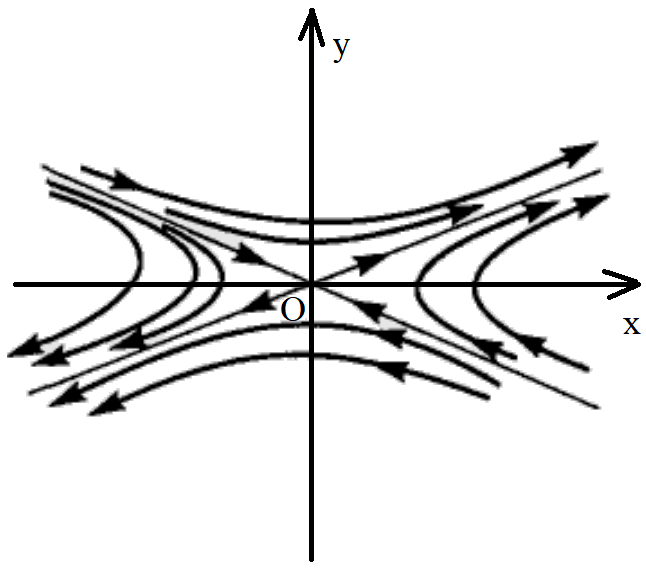
\includegraphics[scale=0.5]{images/seatle.png}$$
$\bullet$ \textit{Точки покоя, в окрестности которых фазовые графики имеют такой вид, называются \textbf{седлом}}.\\\\
\textbf{II группа.} Пусть $\lambda_1, \lambda_2 \in \Rm$, $\lambda_1 \ne \lambda_2$, $\lambda_1\cdot\lambda_2 > 0$. \\
Тогда фазовые графики описываются уравнениями (2.9.2).\begin{enumerate}
	\item Пусть $C_1 \ne 0$, $C_2 = 0$, тогда фазовыми траекториями являются лучи $y = \lambda_1x, x>0$ и $y = \lambda_1x, x<0$.
	\item Пусть $C_1 = 0$, $C_2 \ne 0$, тогда фазовыми траекториями являются лучи $y = \lambda_2x, x>0$ и $y = \lambda_2x, x<0$.
	\item Пусть $C_1 \ne 0$, $C_2 \ne 0$.\begin{enumerate}
		\item Пусть $\lambda_1 < \lambda_2 < 0$. Тогда при $t\ra +\infty$ фазовый график стремится к точке $O(0, 0)$. А при $t\ra -\infty$ уходит в бесконечность.\\
		Найдем асимптоты. $k = \lim\limits_{t\ra +\infty}\dfrac{y}{x} = \lambda_2$. Следовательно, прямая $y = \lambda_2 x$ является асимптотой. При $t\ra -\infty$ $k = \lim\limits_{t\ra -\infty}\dfrac{y}{x} = \lambda_1$, а $b = \lim\limits_{t\ra -\infty} (y-\lambda_1x) = \infty$.
		$$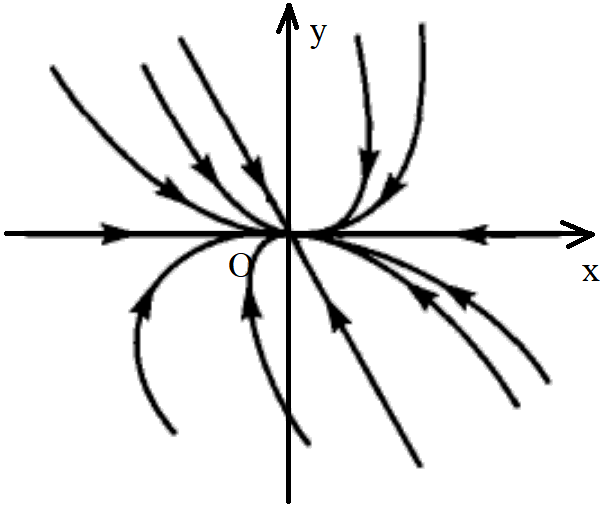
\includegraphics[scale=0.5]{images/in_knot.png}$$
		\item Аналогично можно получить, что фазовые графики для случая $0 < \lambda_1 < \lambda_2$ выглядят следующим образом.
		$$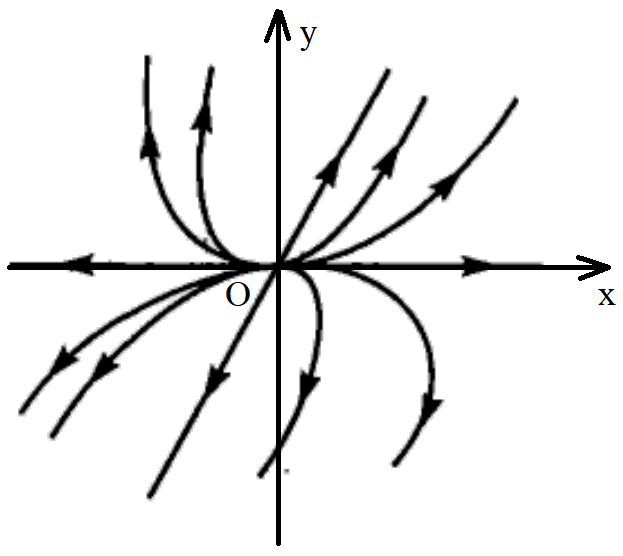
\includegraphics[scale=0.5]{images/out_knot.png}$$
	\end{enumerate}
\end{enumerate}
$\bullet$ \textit{Точка покоя, в окрестности которой фазовый график имеет такой вид, называется \textbf{бикритическим узлом}. Причем \textbf{устойчивым} и \textbf{неустойчивым} соответственно.}\\\\
\textbf{III группа.} Пусть $\lambda_1, \lambda_2 \in \Rm$, $\lambda_1 = \lambda_2 =\lambda$. Тогда фазовые графики решений описываются уравнениями
$$\begin{cases}
	x(t) = C_1e^{\lambda t} + C_2te^{\lambda t} = (C_1 + C_2 t) e^{\lambda t},\\
	y(t) = (C_2 + \lambda C_1 + \lambda C_2t)e^{\lambda t}.
\end{cases}$$\begin{enumerate}
\item Пусть $C_1 \ne 0$, $C_2 = 0$. Исключив из параметрического уравнения $t$, лучи $y = \lambda x$, $x > 0$ и $y = \lambda x$, $x < 0$ являются фазовыми графиками.
\item Пусть $C_2 \ne 0$.\begin{enumerate}
	\item Пусть $\lambda < 0$. Тогда фазовый график при $t \to +\infty$ стремится к точку $O(0,0)$. Если $t \to -\infty$, то фазовый график уходит на бесконечность.\\
	Найдем асимптотические направления:
	$$k = \lim\limits_{t\to+\infty}\dfrac{(C_2 + \lambda C_1 + \lambda C_2t)e^{\lambda t}}{(C_1 + C_2 t) e^{\lambda t}} = \lambda;$$
	$$b = \lim\limits_{t\to+\infty}y(t) - \lambda x(t) = C_2e^{\lambda t} = 0.$$
	Отсюда $y = \lambda x$ --- асимптота фазовых графиков при $t\to+\infty$. Аналогично при $t\to-\infty$ асимптот нет. Прямая $y = \lambda x$ задает асимптотическое направление.
	$$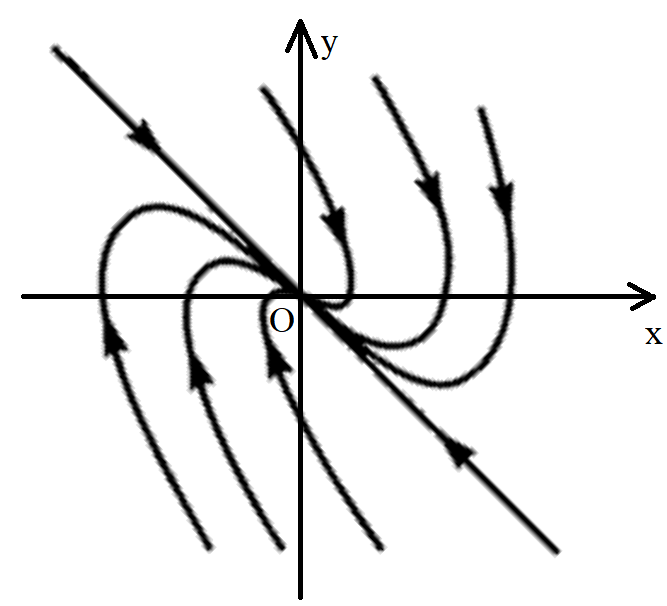
\includegraphics[scale = 0.5]{images/in_monocrit}$$
	\item Пусть $\lambda > 0$. Тогда фазовый график при $t\to+\infty$ уходит на бесконечность, а при $t\to-\infty$ стремится к точке $O(0,0)$. Аналогично фазовый график выглядит следующим образом.
	$$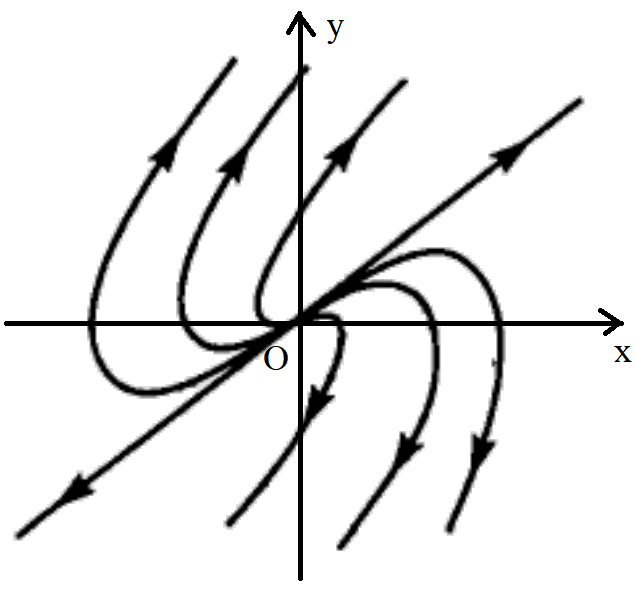
\includegraphics[scale = 0.5]{images/out_monocrit}$$
\end{enumerate}
\end{enumerate}
	$\bullet$ \textit{Точка покоя, в окрестности которой фазовые графики имеют такой вид, называется \textbf{монокритическим узлом}. Причем \textbf{устойчивым} и \textbf{неустойчивым} соответственно.}\\\\
	\textbf{IV группа.} Пусть $\lambda_1, \lambda_2 \in \Cm$, $\lambda = \alpha \pm \beta i$.\begin{enumerate}
		\item Пусть $\alpha \ne 	0$. Тогда фазовые графики описываются уравнениями
		$$\begin{cases}
			x(t) = e^{\alpha t}(C_1\cos(\beta t) + C_2\sin(\beta t)),\\
			y(t) = e^{\alpha t}(C_1\alpha \cos(\beta t) + C_2\alpha \sin (\beta t) - C_1\beta \sin(\beta t) + C_2 \beta \cos(\beta t)).
		\end{cases}$$
	\begin{enumerate}
		\item Если $\alpha < 0$, то фазовый график при $t\to+\infty$ стремится к точке $O(0,0)$, а при $t\to-\infty$ уходит на бесконечность. При этом изменение $t$ от $-\infty$ до $+\infty$ функции $x(t)$ и $y(t)$ меняют знак бесконечное количество раз. Следовательно, графики имеют вид
			$$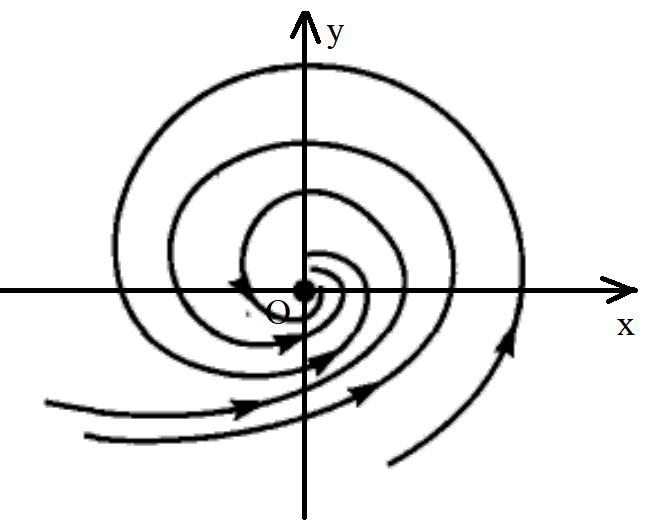
\includegraphics[scale = 0.5]{images/in_focus}$$
		\item Если $\alpha > 0$, то аналогично можно получить, что фазовые графики имеют вид
			$$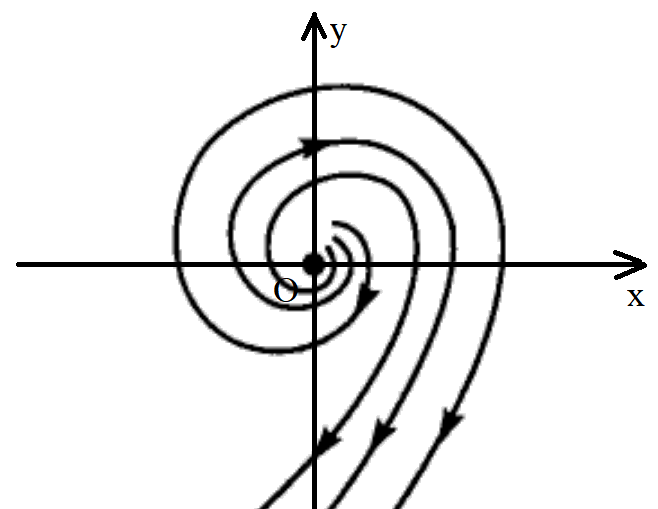
\includegraphics[scale = 0.5]{images/out_focus}$$
	\end{enumerate}
	$\bullet$ \textit{Точка покоя, в окрестности которой фазовые графики ведут себя таким образом, называются \textbf{фокусом}. Причем \textbf{устойчивым} и \textbf{неустойчивым} соответственно.}\\
	\item Пусть $\alpha = 0$. Тогда фазовые графики описываются уравнениями $$\begin{cases}
		x(t) = C_1\cos(t) + C_2\sin(t),\\
		y(t) = -C_1\beta \sin(\beta t) + C_2\beta \cos(\beta t).
	\end{cases}$$
	Исключим из системы $t$. Тогда 
	\begin{center}
		$\Big(x^2 + \dfrac{y^2}{\beta}\Big)^2 = C_1^2 + \dfrac{C_2^2}{\beta}$ --- эллипс.
	\end{center}
Следовательно, фазовые графики имеют вид
$$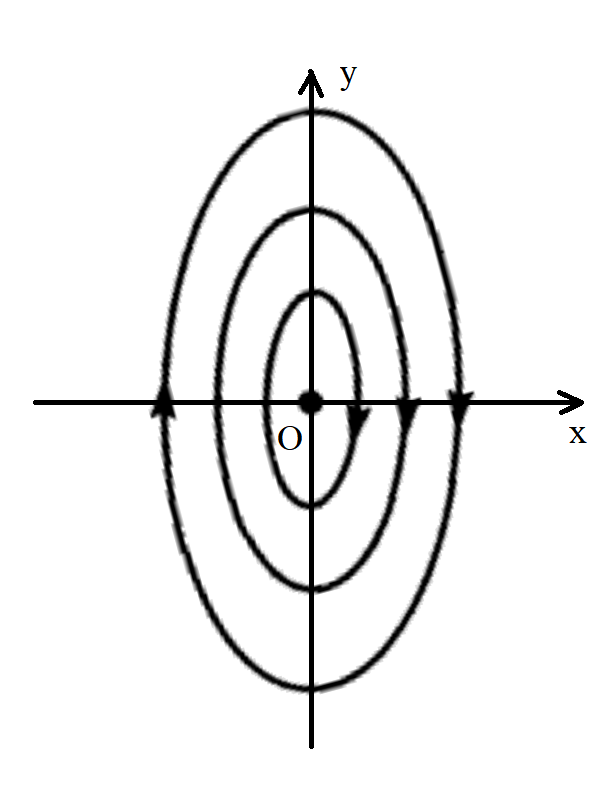
\includegraphics[scale = 0.5]{images/center}$$
$\bullet$ \textit{Точка покоя, в окрестности которой фазовые графики ведут себя таким образом, называется \textbf{центром}.}
	\end{enumerate}
\textbf{V группа.} Пусть среди корней характеристического уравнения есть 0. Тогда в уравнении (1) $a_0 = 0$, и уравнение имеет бесконечно много решений вида $x = C$, фазовые графики которых описываются уравнениями 
$$\begin{cases}
	x = C,\\
	y = 0;
\end{cases}$$
и имеют вид
$$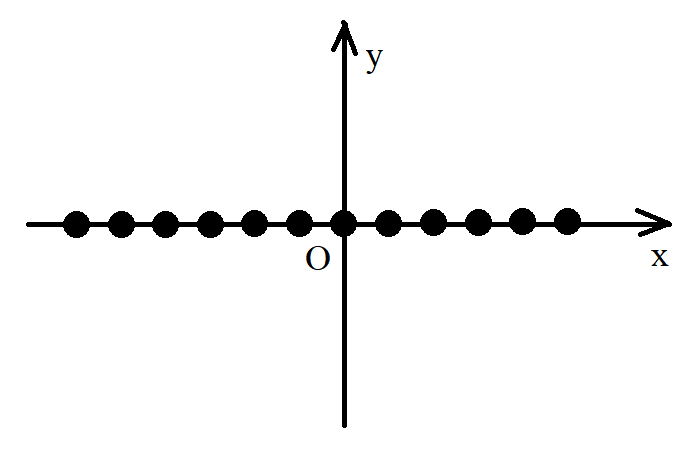
\includegraphics[scale = 0.5]{images/dots_line}$$
Следовательно, каждая точка оси $Ox$ является точкой покоя.\\\\
$\bullet$ \textit{Прямая, каждая точка которой является фазовым графиком, называется \textbf{прямой покоя}.}
\begin{enumerate}
	\item Пусть $\lambda_1 = 0$, $\lambda_2 \ne 0$. Тогда фазовые графики описываются уравнениями
	$$\begin{cases}
		x(t) = C_1 + C_2e^{\lambda t},\\
		y(t) = \lambda C_2e^{\lambda t}.
	\end{cases}$$
Исключив из системы $t$, получим $y = \lambda(x - C_1)$. Получаем, что фазовые графики имеют вид\\
$\lambda < 0$
$$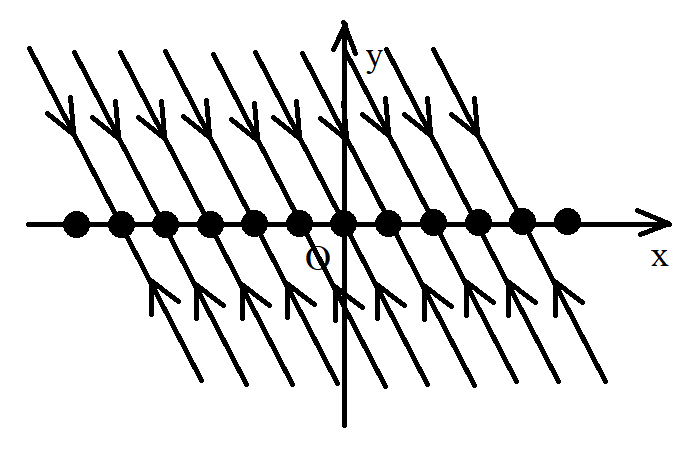
\includegraphics[scale = 0.5]{images/dots_line_in_arrows}$$
$\lambda > 0$
$$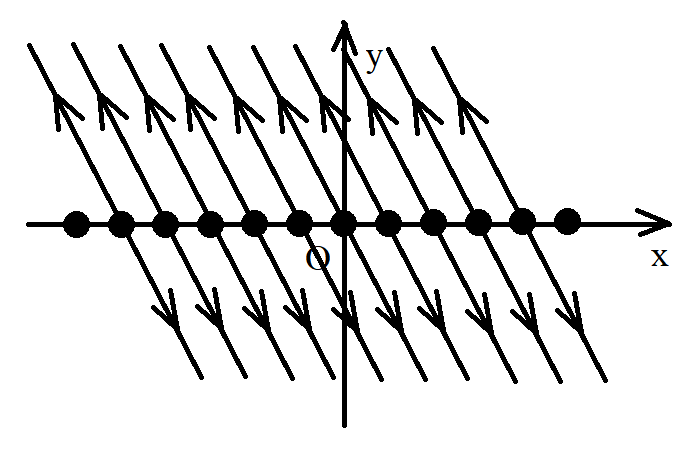
\includegraphics[scale = 0.5]{images/dots_line_out_arrows}$$
\item Пусть $\lambda_1 = \lambda_2 = 0$. Тогда фазовые графики описываются уравнениями
$$\begin{cases}
	x(t) = C_1 + C_2t,\\
	y(t) = C_2.
\end{cases}$$
Следовательно, фазовые графики имеют вид
$$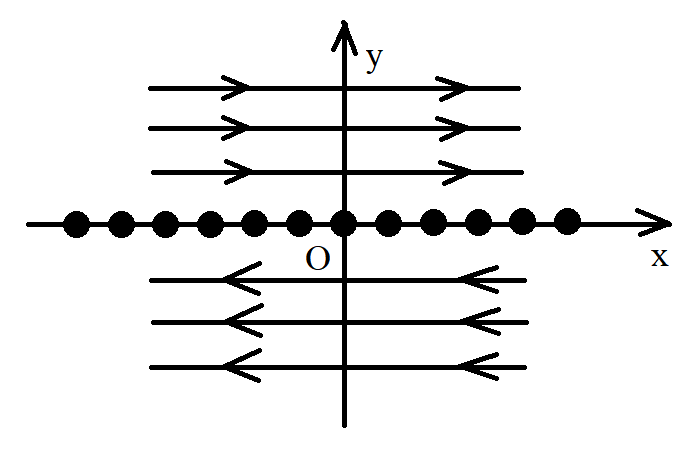
\includegraphics[scale = 0.5]{images/dots_line_lines}$$
\end{enumerate}
\chapter{Линейные стационарные векторные уравнения.}
\section{Системы стационарных линейных уравнений.}
$\bullet$ \textit{\textbf{Системой дифференциальных уравнений} называется совокупность выражений вида
$$F_i(t,x_1(t), Dx_1, \ldots, D^{m_1}x_1, x_2(t), Dx_2,\ldots,D^{m_2}x_2,\ldots,x_k(t),D^kx,\ldots,D^{m_k}x_k) = 0,$$ $$i = 1,\ldots,s,\quad t\in \I\subseteq \Rm,$$ где $F_i$ --- некоторая функция от своих $(m_1+\ldots+m_k + k + 1)$ переменных.}\\\\
$\bullet$ \textit{Говорят, что система дифференциальных уравнений \textbf{имеет нормальную форму}, если она состоит из уравнений вида $$D^{m_i}x_i(t) = f_i(t,x_1(t),Dx_1,\ldots,D^{m_1-1}x_1, \ldots, x_k(t), Dx_k, \ldots, D^{m_k - 1}x_k),\quad i = 1,\ldots, k.$$}
$\bullet$ \textit{Если функции $f_i$ являются линейными функциями от неизвестных функций $x_i(t)$ и их производных, то система называется \textbf{линейной}.}\\\\
Линейную систему из $k$ уравнений можно заменить эквивалентной ей системой из $m_1+\ldots +m_k$ линейных уравнений первого порядка. Следовательно, любое линейное уравнение можно свести к системе из $k$ уравнений.\\\\
Таким образом, в дальнейшем будем рассматривать лишь системы следующего вида
$$\begin{cases}
	Dx_1=a_{11}(t)\cdot x_1(t) + \ldots + a_{1n}(t)\cdot x_n(t) + f_1(t),\\
	\dotfill\\
	Dx_n=a_{n1}(t)\cdot x_1(t) + \ldots + a_{nn}(t)\cdot x_n(t) + f_n(t);
\end{cases}\quad t \in \I.\eqno(3.1.1)$$
$\bullet$ \textit{\textbf{Решением} системы $(3.1.1)$ называется совокупность непрерывно дифференцируемых на $\I$ функций $x_1(t),\ldots, x_n(t)$, обращающих систему $(3.1.1)$ в верное равенство.}\\\\
$\bullet$ \textit{Если коэффициенты систем $(3.1.1)$ являются постоянными, то системы называются \textbf{стационарными линейными}.}\\\\
$\bullet$ \textit{\textbf{Задачей Коши} для системы $(3.1.1)$ называется задача отыскания решения системы $(3.1.1)$, удовлетворяющего условиям
$$x_1|_{t = t_0} = \xi_1, x_2|_{t = t_0} = \xi_2, \dots, x_n|_{t = t_0} = \xi_{n},\quad t_0 \in \I.$$}\\\\
Обозначив $X(t) = \begin{pmatrix}
	x_1(t)\\\vdots\\x_n(t)
\end{pmatrix}$, $DX(t) = \begin{pmatrix}
Dx_1(t)\\\vdots\\Dx_n(t)
\end{pmatrix}$, $A=(a_{ij})$, $f(t) = \begin{pmatrix}
f_1(t)\\\vdots\\f_n(t)
\end{pmatrix}$,  систему (3.1.1) можно записать в матричном виде $$DX = AX + f(t).\eqno(3.1.2)$$
А начальные условия задачи Коши в виде $X|_{t=t_0} = \xi$, где $\xi = \begin{pmatrix}
	\xi_1\\\vdots\\\xi_n
\end{pmatrix}$.\\\\
$\bullet$ \textit{Уравнение $(3.1.2)$ называется \textbf{линейным стационарным векторным уравнением}.}\\\\
$\bullet$ \textit{Если в уравнении $(3.1.2)$ матрицы $X$, $A$, $f$ являются комплекснозначными, то уравнение называется \textbf{комплекснозначным}.}
\begin{lem}
	Задача Коши для комплекснозначного уравнения 
	$$DZ = CZ + h(t), \quad Z|_{t=t_0} = \xi\eqno (3.1.3)$$ с треугольной матрицей $C \in \Cm_{n,n}$ и непрерывной на $\I$ комплекснозначной функцией $h(t)$ имеет единственное решение $\forall t_0 \in \I$, $\forall \xi \in \Cm_{n,1}.$
\end{lem} \begin{Proof}
Пусть $C$ --- нижняя треугольная матрица. Тогда задача Коши (3.1.3) в координатной форме имеет вид
$$\begin{cases}
	Dz_1 = c_{11}z_1 + h_1(t),\\
	Dz_2 = c_{21}z_1 + c_{22}z_2 + h_2(t),\\
	\dotfill\\
	Dz_n = c_{n1}z_1 + c_{n2}z_2 + \ldots + c_{nn}z_n + h_n(t);
\end{cases},\quad \begin{cases}
z_1|_{t=t_0} = \xi_1,\\
z_2|_{t=t_0} = \xi_2,\\
\dotfill\\
z_n|_{t=t_0} = \xi_n.\\
\end{cases}$$
Из первого уравнения следует, что $z_1(t)$ --- решение задачи Коши для линейного стационарного уравнения первого порядка. Такое решение всегда существует и единственно. Подставим его во второе уравнение. Получим, что $z_2(t)$ также решение стационарного линейного уравнения первого порядка, которое также существует и единственно. Продолжая далее аналогично, построим векторную функцию $z(t)$, которая является единственным решением задачи Коши (3.1.3).\\\\
Лемма для верхней треугольной матрицы доказывается аналогично, начиная с последнего уравнения.
\end{Proof}
\begin{theorem}
	Задача Коши для действительного стационарного уравнения $$DX = AX + f(t),\quad X|_{t=t_0} = \xi\eqno(3.1.4)$$ с непрерывной на $\I$ векторной функцией $f(t)$ имеет единственное решение $\forall t_0 \in \I$, $\forall \xi~\in~\Rm_{n,1}.$
\end{theorem}\begin{Proof} Любая действительная матрица $A$ над полем $\Cm$ имеет жорданову нормальную форму, то есть подобную ей комплексную жорданову матрицу $J \in \Cm_{n,n}$. То есть существует невырожденная матрица $S(s_{ij}) \in \Cm_{n,n} : J = S^{-1}AS$. Сделаем в уравнении (3.1.4) замену $X = SZ$. Тогда $$D(SZ) = D\begin{pmatrix}
	s_{11}z_1 + \ldots + s_{1n}z_n\\
	\vdots\\
	s_{n1}z_1 + \ldots + s_{nn}z_n\\
\end{pmatrix} = \begin{pmatrix}
s_{11}Dz_1 + \ldots + s_{1n}Dz_n\\
\vdots\\
s_{n1}Dz_1 + \ldots + s_{nn}Dz_n\\
\end{pmatrix} = SDZ.$$
Тогда $SDZ = ASZ + f(t)$, $SZ|_{t=t_0} = \xi$.\\\\
Домножим полученные уравнения на $S^{-1}$ и получим
$$DZ = \underbrace{S^{-1}AS}_{J}Z + S^{-1}f(t),\quad Z|_{t=t_0} = S^{-1}\xi.$$
В результате получили задачу Коши для комплекснозначного уравнения с матрицей $J$, которая является треугольной, так как жорданова матрица треугольная. По лемме это уравнение имеет единственное решение $Z(t)$. Следовательно, функция $X(t) = SZ(t)$ является решением исходной задачи Коши (3.1.4).\\\\
Но в общем случае это решение является комплекснозначным, то есть имеет вид $$X(t) = U(t) + iV(t),$$ где $U(t)$ и $V(t)$ --- действительные векторные функции. Подставим это выражение в уравнение (3.1.4):
$$DU + iDV = \underset{\in \Rm}{A}(U+ iV) + \underset{\in \Rm}{f(t)},\quad (U+iV)|_{t=t_0} = \underset{\in \Rm}{\xi}.$$
Приравняем в полученном равенстве действительные части слева и справа:
$$DU = AU + f(t),\quad U|_{t=t_0} = \xi.$$
Следовательно, векторная функция $U(t) = Re(X(t))$ является единственным решением задачи Коши (3.1.4).
\end{Proof}
\section{Структура множества решений линейной стационарной системы однородных уравнений.}
Рассмотрим стационарное линейное уравнение 
$$DX = AX,\quad X = \begin{pmatrix}
	x_1\\\vdots\\x_n
\end{pmatrix},\quad A \in \Rm_{n,n}.\eqno(3.2.1)$$
И пусть $X_1(t)$ и $X_2(t)$ --- два решения уравнения (3.2.1). Тогда $$D(\alpha X_1 + \beta X_2) = \alpha DX_1 + \beta DX_2 = \alpha A X_1 + \beta A X_2 = A(\alpha X_1 + \beta X_2) \quad \forall \alpha, \beta \in \Rm$$ И, следовательно, векторная функция $\alpha X_1 + \beta X_2$ также является решением уравнения (3.2.1). Таким образом, множество решений системы (3.2.1) является \textbf{векторным пространством}.\\\\
$\bullet$ \textit{Пусть $X_1(t) = \begin{pmatrix}
	x_{11}(t)\\\vdots\\x_{n1}(t)
\end{pmatrix}$, $\ldots$, $X_n(t) = \begin{pmatrix}
x_{1n}(t)\\\vdots\\x_{nn}(t)
\end{pmatrix}$ --- некоторые векторные функции.
Определитель $$W(t) = \begin{vmatrix}
	x_{11}(t) & \dots & x_{1n}(t)\\
	\vdots & \ddots & \vdots\\
	x_{n1}(t) & \dots & x_{nn}(t)\\
\end{vmatrix}$$ называется \textbf{определителем Вронского} системы $X_1,\ldots,X_n$.}
\begin{theorem}
	Если векторные функции  $X_1,\ldots,X_n$ линейно зависимы, то их $W(t) = 0$ $\forall t$.
\end{theorem}
\begin{Proof}
	Если эти функции линейно зависимы, то одна из них линейно выражается через остальные. Следовательно, один из столбцов определителя равен линейной комбинации остальных столбцов. Тогда $W(t) = 0$.
\end{Proof}
\begin{theorem}
	Если определитель Вронского системы решений  $X_1,\ldots,X_n$ равен нулю хотя бы в одной точке $t_0$, то эти векторные функции линейно зависимые.
\end{theorem}\begin{Proof}
Пусть $\exists t_0 \in \Rm : W(t_0)$ системы решений $X_1,\ldots,X_n$ равен нулю. Следовательно, ранг Вронскиана меньше его порядка и столбцы этой матрицы линейно зависимые. То есть существует нетривиальная линейная комбинация $$\alpha_1X_1(t_0) + \ldots +  \alpha_nX_n(t_0) = 0.$$ Рассмотрим решение $$X(t) =  \alpha_1X_1(t) + \ldots +  \alpha_nX_n(t).$$ Так как столбец $X(t)$ является линейной комбинацией решений уравнения (3.2.1), то он также является решением уравнения (3.2.1) и при этом $$X|_{t=t_0} =  \alpha_1X_1(t_0) + \ldots +  \alpha_nX_n(t_0) = 0.$$
Заметим, что векторная функция $Y(t)\equiv 0$ также является решением уравнения (3.2.1), удовлетворяющим тем же начальным условиям. По теореме о существовании и единственности решения задачи Коши $Y(t) = X(t)$, то есть $X(t)\equiv 0$ и, следовательно, решения $X_1,\ldots,X_n$ линейно зависимые.
\end{Proof}
\begin{cor}
	Если определитель Вронского решений системы $(3.2.1)$ равен нулю при некотором $t_0$, то он равен нулю при любом $t$.
\end{cor}\begin{Proof}
Если при некотором $t_0$ вронскиан $W(t_0) = 0 $, то по второй теореме решения линейно зависимые. Следовательно, по первой теореме $W(t) = 0$ $\forall t$.
\end{Proof}\begin{cor}
Если система решений уравнения $(3.2.1)$ линейно независимая, то их $W(t) \ne 0$ $\forall t$.
\end{cor}\begin{Proof}
Следует из второй теоремы.
\end{Proof}\\\\
Рассмотрим $n$ задач Коши $DX = AX$, $X|_{t=t_0} = E_i$, где $E_i$ --- $i$-ый столбец единичной матрицы $E = [E_1,\ldots, E_n]$. По теореме о существовании и единственности решения задачи Коши все эти задачи Коши имеют единственные решения. Обозначим их $X_1(t),\ldots,X_n(t)$. Вронскиан этой системы решений при $t=t_0$ равен $\det E = 1\ne 0$. Следовательно, эти решения линейно независимые.\\\\ Покажем, что любое решение уравнения (3.2.1) является линейной комбинацией этих решений.
Пусть $X(t)$ --- произвольное решение уравнения (3.2.1) и пусть $$X(t_0) = \xi = \begin{pmatrix}
	\xi_1 \\ \vdots \\ \xi_n
\end{pmatrix} \in \Rm_{n,1}.$$ Рассмотрим векторную функцию $Y(t) = \xi_1X_1 + \ldots + \xi_nX_n$. Так как $Y(t)$ --- линейная комбинация решений системы (3.2.1), то $Y(t)$ --- также решение и при этом $$Y(t_0) = \xi_1X_1(t_0) + \ldots + \xi_nX_n(t_0) = \xi_1\begin{pmatrix}
1\\0\\\vdots\\0
\end{pmatrix} + \xi_2\begin{pmatrix}
0\\1\\\vdots\\0
\end{pmatrix} + \ldots + \xi_n\begin{pmatrix}
0\\0\\\vdots\\1
\end{pmatrix} = \begin{pmatrix}
\xi_1 \\ \vdots \\ \xi_n
\end{pmatrix}.$$
То есть $X(t)$ и $Y(t)$ являются решениями одной задачи Коши. Тогда по теореме о существовании и единственности решения задачи Коши $X(t) = Y(t) = \xi_1X_1 + \ldots + \xi_nX_n$. Следовательно, $X_1,\ldots,X_n$ --- базис пространства решений системы (3.2.1). Таким образом, общее решение имеет вид $$X_{\text{OP}}(t) = C_1X_1 + \ldots + C_nX_n,\quad \forall C_i \in \Rm.$$
$\bullet$ \textit{Базис пространства решений однородного уравнения $(3.2.1)$ называется \textbf{фундаментальной системой решений}.}\\\\
$\bullet$ \textit{Матрица $\FI(t) = [X_1(t),\ldots,X_n(t)]$ называется \textbf{фундаментальной матрицей} системы $(3.2.1)$.}\\\\
Фундаментальная матрица невырожденная при любом $t$.\\\\
$\bullet$ \textit{Фундаментальная система решений называется \textbf{нормированной при $t = t_0$}, если ее $\FI(t_0) = E$.}\\\\
Общее решение уравнения (3.2.1) в матричном виде с использованием фундаментальной матрицы может быть записано следующим образом: $$X_{\text{OP}}(t) = \FI(t)\cdot C, \quad \forall C \in \Rm_{n,1}.$$
Если $X(t)$ --- решение задачи Коши $DX = AX$, $X|_{t=t_0} = \xi$, то $X(t_0) = \FI(t_0)\cdot C = \xi$. Так как матрица $\FI(t_0)$ невырожденная, то $\exists \FI^{-1}(t_0) : C = \FI^{-1}(t_0)\xi$. Следовательно, решение задачи Коши имеет вид $$X(t) = \FI(t)\cdot \FI^{-1}(t_0)\xi.$$
\section{Метод Эйлера построения фундаментальной системы решений линейных векторных уравнений.}
Рассмотрим линейное векторное уравнение $$DX = AX, \quad t\in \Rm. \eqno(3.3.1)$$
Найдем решение этого уравнения в виде $$X(t) = B_0e^{\lambda t},\eqno(3.3.2)$$ где $B_0$ --- некоторый ненулевой столбец ($B_0\in \Rm_{n,1}$). Подставим функцию (3.3.2) в уравнение (3.3.1): 
$$\lambda B_0 e^{\lambda t} = A B_0 e^{\lambda t}\Longleftrightarrow AB_0 - \lambda B_0 = 0\Longleftrightarrow (A-\lambda E)B_0 = 0.$$
Столбец $B_0$ является ненулевым решением полученного матричного уравнения, если $\det (A-\lambda E) = 0$. Следовательно, $\lambda$ --- собственное значение матрицы $A$, а $B_0$ --- собственный вектор, соответствующий этому значению.\\\\
Таким образом, функция (3.3.2) является ненулевым решением уравнения (3.3.1), если $B_0$ --- собственный вектор, $\lambda$ --- собственное значение.\\\\ Если матрица $A$ является матрицей простой структуры, то существует базис пространства $\Rm_{n,1}$ составленный из собственных векторов матрицы $A$. Тогда, используя этот базис, можем построить $n$ решений вида $(3.3.2)$ системы $(3.3.1)$, которые являются линейно независимыми, так как определитель Вронского этой системы решений при $t = 0$ равен определителю матрицы, составленной из $n$ линейно независимых собственных векторов, а значит не равен нулю.\\\\
Если матрица $A$ не является матрицей простой структуры, то для нее всегда существует в общем случае комплексная подобная жорданова матрица, а следовательно для этой матрицы существует в общем случае комплексный жордановый базис.
\begin{theorem}
	Если $B_0, B_1, \ldots, B_k$ --- жорданова цепочка матрицы $A$, соответствующая собственному значению $\lambda_0$, то векторная функция $$X(t) = \Big(B_0\dfrac{t^k}{k!} + B_1\dfrac{t^{k-1}}{(k-1)!} + B_2\dfrac{t^{k-2}}{(k-2)!} + \ldots + B_{k-1}\dfrac{t}{1!} + B_k\Big)\cdot e^{\lambda_0 t}\eqno (3.3.3)$$ является решением уравнения $(3.3.1)$. 
\end{theorem}\begin{Proof}
Вычислим для векторной функции (3.3.3) векторную функцию $AX - DX$:\begin{multline*}
	AX - DX = A\Big(B_0\dfrac{t^k}{k!} + B_1\dfrac{t^{k-1}}{(k-1)!} + \ldots + B_{k-1}\dfrac{t}{1!} + B_k\Big)\cdot e^{\lambda_0 t} - \Big(B_0\dfrac{t^{k-1}}{(k-1)!} +\\+ B_1\dfrac{t^{k-2}}{(k-2)!} + \ldots + B_{k-1}\Big)\cdot e^{\lambda_0 t} -\lambda_0\Big(B_0\dfrac{t^k}{k!} + B_1\dfrac{t^{k-1}}{(k-1)!} + \ldots + B_{k-1}\dfrac{t}{1!} + B_k\Big)\cdot e^{\lambda_0 t}
\end{multline*}
Сравним коэффициенты:\\
$t^ke^{\lambda_0 t} : AB_0\dfrac{1}{k!} - \lambda_0B_0\dfrac{1}{k!} = \dfrac{1}{k!}(A-\lambda_0E)B_0 = 0$, так как $B_0$ --- собственный вектор, соответствующий собственному значению $\lambda_0$.\\
$t^{k-1} e^{\lambda_0 t}: \dfrac{1}{(k-1)!}AB_1 - \dfrac{1}{(k-1)!}B_0 - \dfrac{1}{(k-1)!}\lambda_0B_1 = \dfrac{1}{(k-1)!}(AB_1-\lambda_0B_1 - B_0) =\\ \dfrac{1}{(k-1)!}(\underbrace{(A-\lambda_0E)B_1}_{B_0}- B_0) = 0$, так как $B_1$ --- вектор присоединенный к $B_0$.\\
Продолжая аналогично, получим, что $AX - DX = 0$. Следовательно, $DX = AX$, то есть $X$ --- решение уравнения (3.3.1).
\end{Proof}\\\\
Так как для жордановой цепочки $B_0,\ldots, B_k$ длины $(k+1)$ любая ее подсистема $B_0, B_1, \ldots, B_m$, $0\leqslant m \leqslant k$, также является жордановой цепочкой, то, используя жоданову цепочку длины $(k+1)$, можно построить $(k+1)$ решение системы (3.3.1).\\\\
Следовательно, используя жорданов базис матрицы $A$ составленный из жордановых цепочек, можно построить ровно $n$ различных решений уравнения (3.3.1).\\\\
Если вычислить значение фундаментальной матрицы составленной из этих решений при $t=0$, получим матрицу, состоящую из жорданового базиса матрицы $A$, которая невырожденная. Следовательно, построенная система решений линейно независимая.\\\\
Если среди собственных значений матрицы $A$ существуют мнимые, то собственные и присоединенные векторы, соответствующие этим собственным значениям, также мнимые. И построенные решения являются комплекснозначными. Но так как матрица $A$ действительная, их действительные и мнимые части являются линейно независимыми действительными решениями. Следовательно, используя комплексное собственное значение кратности $k$ можно построить $2k$ линейно независимых действительных решений. При этом аналогично построенные решения для сопряженного мнимого значения новыми независимыми решениями не являются. 
\section{Матричный метод построения фундаментальной системы решений линейных стационарных векторных уравнений.}
Рассмотрим уравнение $$DX = AX,\eqno(3.4.1)$$ где $A$ --- матрица $n\times n$, $X$ --- вектор-функция. Пусть $\{A_i\}_{i=0}^\infty$ --- последовательность матриц одного порядка.\\\\
$\bullet$ \textit{Матрица $A$ называется \textbf{пределом} этой последовательности, если $$\forall \upvarepsilon\ \exists N : \forall i > N \quad \left\| A - A_i\right\| < \upvarepsilon.$$ }
$\bullet$ \textit{Ряд $\sum\limits_{i=0}^{\infty}A_i$ называется \textbf{сходящимся}, если существует предел частных сумм.}\\\\
Матричный ряд сходится $\Longleftrightarrow$ сходятся все ряды, образованные из соответствующих элементов этих матриц.\\\\
Рассмотрим ряд $$E + \dfrac{A}{1!}+\dfrac{A^2}{2!} + \ldots + \dfrac{A^k}{k!} + \ldots. \eqno (3.4.2)$$
Модуль любого элемента матрицы $A^k$ не превосходит $\left\| A^k \right\|$, которая по определению матричной нормы не превосходит $\left\| A \right\|^k$, то есть
$$A^k \leq \Norm{A^k} \leq \Norm{A}^k.$$
Тогда ряды, состоящие из соответствующих элементов матриц $\dfrac{A^i}{i!}$, имеют сходящуюся числовую мажоранту $$1 + \dfrac{\left\| A \right\|}{1!} + \dfrac{\left\| A \right\|^2}{2!} + \ldots = e^{\left\| A \right\|},$$ а, следовательно, являются сходящимися.\\\\
$\bullet$ \textit{Ряд $(3.4.2)$ также является сходящимся матричным рядом, обозначается $e^A$ и называется \textbf{матричной экспонентой}}.\\\\
Ряд (3.4.2) является сходящимся для любой матрицы $A$.\\\\
\textbf{\textit{Свойства матричной экспоненты:}}
\begin{enumerate}
	\item $e^0 = E$\textit{ $(0$ --- нулевая матрица$)$.}
	\item \textit{Если матрицы $A$, $B$ перестановочны, то есть $AB = BA$, то $e^A \cdot e^B = e^{A+B}$.}
	\begin{Proof}
		\begin{multline*}
			e^A\cdot e^B = \Big(E + \dfrac{A}{1!}+\dfrac{A^2}{2!} + \dfrac{A^3}{3!} + \ldots \Big)\Big(E + \dfrac{B}{1!}+\dfrac{B^2}{2!} + \dfrac{B^3}{3!} + \ldots \Big) =\\= E + \Big(\dfrac{A}{1!} + \dfrac{B}{1!}\Big) + \Big(\dfrac{A^2}{2!}+\dfrac{A\cdot B}{1!} + \dfrac{B^2}{2!}\Big) + \ldots = E + \dfrac{A+B}{1!} + \dfrac{A^2 + 2AB + B^2}{2!} + \ldots =\\= [AB = BA, \text{иначе свернуть нельзя}] = E + \dfrac{A+B}{1!} + \dfrac{(A+B)^2}{2!} + \ldots = e^{A+B}.
		\end{multline*}
	\end{Proof}
\item $(e^A)^{-1} = e^{-A}$.
\begin{Proof}
	Так как матрицы $A$ и $-A$ перестановочны, то по второму свойству $$e^A\cdot e^{-A} = e^{A - A} = e^0 = E.$$
\end{Proof}
\end{enumerate}
Рассмотрим матричную экспоненту $$e^{At} = E + \dfrac{A}{1!}t+\dfrac{A^2}{2!}t^2 + \ldots + \dfrac{A^k}{k!}t^k + \ldots,\eqno(3.4.3)$$
где $t$ --- некоторая действительная переменная. При любом фиксированном $t$ ряд (3.4.3) является сходящимся. На любом ограниченном промежутке ряд (3.4.3) является равномерно сходящимся, так как для него существует сходящийся числовой мажорирующий ряд. Тогда $$D(e^{At}) = A +\dfrac{2A^2}{2!}t + \dfrac{3A^3}{3!}t^2+ \ldots= A\Big(E + \dfrac{A}{1!}t+\dfrac{A^2}{2!}t^2 + \ldots\Big) = Ae^{At} = e^{At}A.$$
\begin{theorem}
	Задача Коши $DX = AX$, $X|_{t=t_0} = \xi$, $t_0 \in \Rm$, $\xi \in \Rm_{n,1}$ имеет единственное решение $$X(t) = e^{A(t-t_0)}\xi.$$
\end{theorem}
\begin{Proof}
	Задача Коши имеет единственное решение по теореме о существовании и единственности решения задачи Коши.\\\\
	Покажем, что вектор-функция $X(t)$ является этим решением: $$DX = D(e^{A(t-t_0)}\xi) = D(e^{At}e^{-At_0}\xi) = D(e^{At})e^{-At_0}\xi = Ae^{At}e^{-At_0}\xi  = Ae^{A(t-t_0)}\xi = AX(t),$$ то есть $X(t)$ --- решение. И при этом $X|_{t=t_0} = e^{A(t-t_0)}\xi = e^{A\cdot 0}\xi = e^0\xi = E\xi = \xi$.
\end{Proof}
\begin{cor}
	Матрица $e^{A(t-t_0)}$ является фундаментальной матрицей уравнения $(3.4.1)$, нормированной в точке $t =t_0$.
\end{cor}\begin{Proof}
Так как $i$-ый столбец матрицы $e^{A(t-t_0)}$ представим в виде $e^{A(t-t_0)}\begin{pmatrix}
	0\\\vdots\\0\\1\\0\\\vdots\\0
\end{pmatrix}i$, то он является решением задачи Коши для уравнения (3.4.1) с начальным условием $X|_{t=t_0} = \begin{pmatrix}
0\\\vdots\\0\\1\\0\\\vdots\\0
\end{pmatrix}$. Следовательно, каждый столбец матрицы $e^{A(t-t_0)}$ --- решение уравнения (3.4.1). При $t=t_0$ матрица $e^{A(t-t_0)} = E$, следовательно, совокупность решений уравнения (3.4.1), образующих матрицу $e^{A(t-t_0)}$, имеет невырожденный вронскиан в точке $t=t_0$. А значит эти решения линейно независимые. То есть матрица $e^{A(t-t_0)}$ фундаментальная. 
\end{Proof}\\\\
Таким образом, общее решение уравнения (3.4.1) имеет вид $$X_\text{OO}(t) = e^{A(t-t_0)}\cdot C,\quad C = \begin{pmatrix}
	C_1\\\vdots\\C_n
\end{pmatrix}.$$
\subsection*{Вычисление матричной экспоненты.}
$\forall A \in \Cm_{n,n}$ $\exists J$ --- жорданова нормальная форма, то есть $\exists$ невырожденная матрица $S: J = S^{-1}AS \Rightarrow A = S JS^{-1}$. Следовательно, \begin{multline*}
	e^{At} = e^{(SJS^{-1})t} = SES^{-1} + \dfrac{SJS^{-1}}{1!}t + \dfrac{SJS^{-1}SJS^{-1}}{2!}t^2 + \ldots =\\= S\cdot \Big(E + \dfrac{J}{1!}t + \dfrac{J^2}{2!}t^2 + \dfrac{J^3}{3!}t^3 + \ldots\Big)\cdot S^{-1} = Se^{Jt}S^{-1}.
\end{multline*}
Пусть $J = \operatorname{diag}[J_1,\ldots,J_k]$, где $J_i$ --- жордановы клетки. Следовательно, $e^{Jt} = \operatorname{diag}(e^{J_1t},\ldots,e^{J_kt})$.\\
Вычислим матричную экспоненту для клетки Жордана:
$$J = \begin{pmatrix}
	\lambda & 1 & \dots & 0\\
	\vdots & \vdots & \ddots & \vdots\\
	0 & 0 & \dots & 1\\
	0 & 0 & \dots & \lambda
\end{pmatrix};\quad J^2 = \begin{pmatrix}
\lambda^2 & 2\lambda & 1 & \dots & 0\\
\vdots & \vdots & \vdots & \ddots & \vdots\\
0 & 0 & 0 & \dots & 1\\
0 & 0 & 0 & \dots & 2\lambda\\
0 & 0 & 0 & \dots & \lambda^2
\end{pmatrix};\quad J^3 = \begin{pmatrix}
\lambda^3 & 3\lambda^2 & 3\lambda & 1 & \dots & 0\\
\vdots & \vdots & \vdots & \ddots & \vdots\\
0 & 0 & 0 & 0 & \dots & 1\\
0 & 0 & 0 & 0 & \dots & 3\lambda\\
0 & 0 & 0 & 0 & \dots & 3\lambda^2\\
0 & 0 & 0 & 0 & \dots & \lambda^3
\end{pmatrix}.$$
Тогда первый элемент матрицы $e^{Jt}$ равен $$1 + \dfrac{\lambda}{1!}t + \dfrac{\lambda^2}{2!}t^2 + \dfrac{\lambda^3}{3!}t^3 + \ldots = e^{\lambda t}.$$
Второй элемент матрицы $e^{Jt}$ равен $$0 + \dfrac{1}{1!}t + \dfrac{2\lambda}{2!}t^2 + \dfrac{3\lambda^2}{3!}t^3 + \ldots  = t \Big(1 + \dfrac{\lambda}{1!}t + \dfrac{\lambda^2}{2!}t^2 + \dfrac{\lambda^3}{3!}t^3 + \ldots\Big)= te^{\lambda t}.$$
Следующий элемент будет равен $\dfrac{t^2}{2!}e^{\lambda t}$. И так далее. В итоге получим
$$e^{Jt} = e^{\lambda t}\begin{pmatrix}
	1 & \dfrac{t}{1!} & \dfrac{t^2}{2!} & \dfrac{t^3}{3!} & \dots\\
	0 & 1 & \dfrac{t}{1!} & \dfrac{t^2}{2!} & \dots\\
	0 & 0 & 1 & \dfrac{t}{1!} & \dots\\
	0 & 0 & 0 & 1 & \dots\\
	\vdots & \vdots & \vdots & \vdots & \ddots
\end{pmatrix}$$
\section{Неоднородные стационарные линейные векторные уравнения.}
Рассмотрим уравнение $$DX = AX + f(t),\quad t \in \I\eqno(3.5.1)$$
с непрерывной на $\I$ векторной функцией $f(t)$ и соответствующее ему однородное уравнение $$DX = AX.\eqno(3.5.2)$$
\begin{theorem}
	Если $X_1(t)$ --- некоторое решение уравнения $(3.5.1)$, то $\forall X_0(t)$ решения уравнения $(3.5.2)$ вектор-функция $X_1 + X_0$ --- решение уравнения $(3.5.1)$.
\end{theorem}
\begin{Proof}
	$D(X_1 + X_0) = DX_1 + DX_0 = AX_1 + f(t) + AX_0 = A(X_1+X_0) + f(t).$
\end{Proof}
\begin{theorem}
	Если $X_1(t)$ --- решение уравнения $(3.5.1)$, то $\forall X_2(t)$ решения уравнения $(3.5.1)$ вектор-функция $X_ 0 = X_2 - X_1$ --- решение уравнения $(3.5.2)$.
\end{theorem}
\begin{Proof}
	$DX_0 = D(X_2 - X_1) = DX_2 - DX_1 = AX_2 + f(t) - (AX_1 + f(t)) = A(X_2 - X_1) = AX_0.$
\end{Proof}\\\\
Из предыдущих теорем следует, что все решения неоднородного уравнения можно получить, прибавив к некоторому частному решению все решения соответствующего однородного уравнения, то есть $$X_\text{OH} = X_\text{OO} + X_\text{ЧН}.$$
Частное решение неоднородного уравнения может быть найдено \textbf{методом вариации произвольной постоянной (методом Лагранжа)}.\\\\
Пусть $\FI(t) = [X_1(t),\ldots,X_n(t)]$ --- фундаментальная матрица уравнения (3.5.2). Частное решение уравнения (3.5.1) будем искать в виде $$X(t) = X_1(t)\cdot u_1(t) + \ldots + X_n(t)\cdot u_n(t),$$ где $u_i(t)$ --- некоторые дифференцируемые функции. Если обозначим $U(t) = \begin{pmatrix}
	u_1(t) \\ \vdots \\ u_n(t)
\end{pmatrix}$, то частное решение можно представить как $$X(t) = \FI(t)\cdot U(t).$$
Подставим функцию $X(t)$ в уравнение (3.5.1):
$$DX_1u_1 + X_1Du_1 + \ldots + DX_nu_n + X_nDu_n = A(X_1u_1 + \ldots + X_nu_n) + f(t).$$
Так как $X_i$ являются решениями уравнения (3.5.2), то $DX_i = AX_i$. Следовательно, $DX_iu_i = AX_iu_i$.
Тогда получаем $$X_1Du_1 + \ldots + X_nDu_n = f(t),$$
в матричном виде $$\FI(t)\cdot DU(t) = f(t).$$
Так как $\FI(t)$ --- фундаментальная матрица уравнения (3.5.2), то ее столбцы --- линейно независимые решения однородного уравнения. Следовательно, определитель фундаментальнй матрицы является вронскианом решений $X_1(t),\ldots, X_n(t)$, а значит $$\det \FI(t) \ne 0\quad \forall t \Rightarrow \exists \FI^{-1}(t) : DU(t) = \FI^{-1}(t) \cdot f(t).$$ Тогда в качестве векторной функции $U(t)$ можно выбрать функцию $$U(t) = \int\limits_{t_0}^t\FI^{-1}(\uptau) f(\uptau)d\uptau,\quad t, t_0 \in \I.$$
Следовательно, общее решение неоднородного уравнения имеет вид $$X_{\text{он}} = \FI(t)\cdot C + \FI(t) \int\limits_{t_0}^t\FI^{-1}(\uptau) f(\uptau)d\uptau = \FI(t)\cdot (C +\int\limits_{t_0}^t\FI^{-1}(\uptau) f(\uptau)d\uptau).\eqno (3.5.3)$$
Используя формулу (3.5.3), найдем решение задачи Коши $DX = AX + f(t)$, $X|_{t=t_0} = \xi$. Для этого подставим в (3.5.3) начальные условия:
$X|_{t=t_0} = \FI(t_0)\cdot C = \xi \Rightarrow C = \FI^{-1}(t_0)\xi.$
Следовательно, решение задачи Коши имеет вид $$X(t) = \FI(t)\cdot \FI^{-1}(t_0)\xi + \FI(t)\int\limits_{t_0}^t\FI^{-1}(\uptau) f(\uptau)d\uptau.$$
В качестве фундаментальной матрицы $\FI(t)$ можно взять матрицу $e^{At}$ ($\FI(t) = e^{At}$). Тогда решение задачи Коши примет вид $$X(t) = e^{A(t-t_0)}\xi + \int\limits_{t_0}^te^{A(t-\uptau)} f(\uptau)d\uptau.\eqno (3.5.4)$$
Из уравнения (3.5.4) следует, что задача Коши для уравнения (3.5.1) с нулевыми начальными условиями ($\xi = 0$) имеет вид $$X(t) = \int\limits_{t_0}^te^{A(t-\uptau)} f(\uptau)d\uptau.\eqno(3.5.5)$$
То есть функция (3.5.5) является частным решением уравнения (3.5.1).\\\\
$\bullet$ \textit{Формула $(3.5.5)$ называется \textbf{методом Коши} отыскания частного решения неоднородного уравнения.}\\\\
Следовательно, общее решение уравнения (3.5.1) можно записать в виде $$X(t) = e^{A(t-t_0)}C + \int\limits_{t_0}^te^{A(t-\uptau)} f(\uptau)d\uptau.$$
\section{Непрерывная зависимость решений стационарного линейного векторного уравнения от начальных значений.}
Рассмотрим уравнение $$DX = AX + f(t),\quad t \in \I\eqno(3.6.1)$$
с непрерывной на $\I$ векторной функцией $f(t)$ и соответствующее ему однородное уравнение $$DX = AX.\eqno(3.6.2)$$
$\bullet$ \textit{Решение $X_0(t)$ уравнения $(3.6.1)$ называется \textbf{непрерывно зависящим} на промежутке $\I$ \textbf{от начальных значений}, если}
\begin{center}
	$\forall \upvarepsilon\ \exists\delta: \forall X(t)$ \textit{решения} $(3.6.1)$ $\left\| X(t_0) - X_0(t_0) \right\| < \delta \Rightarrow \left\| X(t) - X_0(t) \right\| < \upvarepsilon$ $\forall t \in \I$.
\end{center}
$\bullet$ \textit{Функция $\left\| X(t) - X_0(t) \right\|$ называется \textbf{отклонением} $X(t)$ от $X_0(t)$, а ее значение при $t=t_0$, то есть $\left\| X(t_0) - X_0(t_0) \right\|$, называется \textbf{начальным отклонением}.}\\\\
Пусть $X_0(t)|_{t=t_0} = \xi$, а $X(t)|_{t=t_0} = \xi+\Delta \xi$, где $\xi, \Delta\xi \in \Rm_{n,1}.$
Тогда по правилу Коши $$X_0(t) = e^{A(t-t_0)}\xi + \int\limits_{t_0}^te^{A(t-\uptau)} f(\uptau)d\uptau;\quad X(t) = e^{A(t-t_0)}(\xi +\Delta\xi)+ \int\limits_{t_0}^te^{A(t-\uptau)} f(\uptau)d\uptau.$$
Отсюда\begin{itemize}
	\item $X(t) - X_0(t) = e^{A(t-t_0)}\Delta\xi$ --- отклонение;
	\item $X(t_0) - X_0(t_0) = E\Delta\xi$ --- начальное отклонение.
\end{itemize}
Следовательно, отклонение решения $X(t)$ от $X_0(t)$ не зависит от самих решений, а зависит лишь от их начальных отклонений. То есть все решения уравнения (3.6.1) либо одновременно зависят от начальных данных, либо нет. Кроме того отклонение зависит лишь от матрицы $A$ и не зависит от неоднородности $f(t)$. Следовательно, и непрерывная зависимость от начальных данных зависит только от матрицы $A$.
\begin{theorem}
	Если промежуток $\I$ является отрезком, то любое решение уравнения $(3.6.1)$ непрерывно зависит от начальных значений.
\end{theorem}\begin{Proof}
Так как $e^{A(t-t_0)}$ --- фундаментальная матрица уравнения (3.6.2), то все ее компоненты являются непрерывными. Следовательно, по теореме Вейрштрасса на отрезке $\I$ они все являются ограниченными. То есть $$\exists M : \Norm{e^{A(t-t_0)}}\leq M \Rightarrow \Norm{X(t) - X_0(t)} = \Norm{e^{A(t-t_0)}\Delta\xi}\leq\Norm{e^{A(t-t_0)}}\cdot \Norm{\Delta \xi}\leq M \cdot \Norm{X(t_0) - X_0(t_0)}.$$
Таким образом, $$\forall \epsilon\ \exists \delta = \dfrac{\epsilon}{M} : \Norm{X(t_0) - X_0(t_0)} < \delta \Rightarrow \Norm{X(t) - X_0(t)} < M\cdot \delta = M\cdot \dfrac{\epsilon}{M} = \epsilon.$$
\end{Proof}\\
$\bullet$ \textit{Решение уравнения $(3.6.1)$ называется \textbf{интегрально зависящим от начальных значений} на промежутке $\I$, если оно зависит от начальных значений на любом отрезке $I_0 \subseteq\I$.}
\section{Устойчивость стационарных линейных векторных уравнений.}
Рассмотрим уравнение $$DX = AX + f(t),\ t \in \I = [t_0; + \infty)\eqno (3.7.1)$$ с непрерывной на $\I$ векторной функцией $f(t)$.\\\\
$\bullet$ \textit{Решение $X_0(t)$ уравнения $(3.7.1)$ называется \textbf{устойчивым по Ляпунову}, если}$$\forall \epsilon\ \exists\delta : \forall X(t)\quad \Norm{X(t_0) - X_0(t_0)} < \delta \Rightarrow \Norm{X(t) - X_0(t)} < \epsilon\ \forall t > t_0.$$
Таким образом, решение $X_0(t)$ называется устойчивым по Ляпунову, если оно непрерывно зависит от начальных данных на промежутке $\I$ вида $[t_0;+\infty)$.\\\\
$\bullet$ \textit{Если кроме того $$\lim\limits_{t\to+\infty}\Norm{X(t) - X_0(t)} = 0,$$ то решение $X_0(t)$ называется \textbf{асимптотически устойчивым}.}\\\\
Из определения устойчивости и свойств непрерывной зависимости от начальных значений следует, что все решения уравнения $(3.7.1)$ либо одновременно устойчивы, либо нет.\\\\
$\bullet$ \textit{Уравнение, все решения которого устойчивы, называется \textbf{устойчивым} (аналогично \textbf{неустойчивым}, \textbf{асимптотически устойчивым}).}\\\\
Кроме того, так как неоднородность уравнений не влияет на непрерывную зависимость от начальных значений, то и устойчивость уравнения не зависит от неоднородности $f(t)$. Следовательно, в дальнейшем для исследования устойчивости будем исследовать нулевое решение уравнения $$DX = AX.\eqno(3.7.2)$$ То есть\\\\
$\bullet$ \textit{Уравнение называется \textbf{устойчивым}, если} $$\forall \epsilon\ \exists\delta : \forall X(t)\quad \Norm{X(t_0)} < \delta \Rightarrow \Norm{X(t)} < \epsilon\ \forall t > t_0.$$
\begin{lem}
	Уравнение $(3.7.2)$ является устойчивым на $\I$ $\Longleftrightarrow$ каждое его решение является ограниченным на $\I$.
\end{lem}
\begin{Proof}
	$\Rightarrow)$ От противного. Пусть (3.7.2) устойчиво, но $\exists Y(t)$ решение неограниченное на промежутке $\I$. Тогда векторная функция $X(t) = CY(t)$ является также решением уравнения (3.7.2), и при этом, выбирая $C$ сколь угодно малым, можем получить решение, которое при $t=t_0$ будет сколь угодно близко к нулевому решению, но при этом являться неограниченным.\\\\
	$\Leftarrow)$ Пусть все решения уравнения (3.7.2) ограничены на $\I$. Тогда фундаментальная матрица $e^{A(t-t_0)}$ тоже ограничена. То есть $\exists M : \Norm{e^{A(t-t_0)}}\leq M$ $\forall t > t_0$. Тогда $$\forall \epsilon\ \exists \delta = \dfrac{\epsilon}{M} : \forall X(t)=e^{A(t-t_0)}\xi\quad \Norm{X(t_0)} < \delta \Rightarrow \Norm{X(t)} < M\cdot \delta = M\cdot \dfrac{\epsilon}{M} = \epsilon.$$
\end{Proof}
\begin{theorem}
	[Критерий устойчивости]
	Неоднородное уравнение $(3.7.1)$ устойчиво $\Longleftrightarrow$ действительные части собственных значений матрицы $A$ неположительны, при этом собственные значения с нулевой действительной частью имеют равные алгебраические и геометрические кратности.
\end{theorem}\begin{Proof}
Так как неоднородность не влияет на устойчивость, то уравнение (3.7.1) устойчиво $\Longleftrightarrow$ уравнение (3.7.2) устойчиво. А по лемме это уравнение устойчиво $\Longleftrightarrow$ все его решения ограничены.\\\\
Из метода Эйлера построения фундаментальной системы решения однородного уравнения для ограниченности решений необходимо и достаточно, чтобы действительные части собственных значений были неположительны. Причем собственным значениям с нулевой действительной частью в жордановом базисе матрицы $A$ должны соответствовать цепочки длины 1. А это возможно, когда алгебраическая и геометрическая кратности этого собственного значения равны.
\end{Proof}
\begin{cor}
	Неоднородное уравнение $(3.7.1)$ устойчиво $\Longleftrightarrow$ действительные части собственных значений матрицы $A$ неположительны, при этом собственным значениям с нулевой действительной частью в жордановой нормальной форме матрицы $A$ соответствуют клетки порядка $1$.
\end{cor}
\begin{lem}
	Уравнение $(3.7.2)$ является асимптотически устойчивым $\Longleftrightarrow$ все его решения стремятся к нулю при $t \rightarrow + \infty$.
\end{lem}
\begin{Proof}
	$\Rightarrow)$ Пусть уравнение асимптотически устойчиво. Тогда и его нулевое решение асимптотически устойчиво, то есть $$\forall \epsilon\ \exists \delta : \forall X(t) \quad \Norm{X(t_0)} < \delta \Rightarrow \lim\limits_{t\to +\infty} \Norm{X(t)} = 0.$$
	Пусть $Y(t)$ --- произвольное решение уравнения (3.7.2). Тогда векторная функция $CY(t)$, $C \in \Rm$ также является решением уравнения (3.7.2). Причем, выбирая $C$ достаточно малым, можно получить решение сколь угодно близкое к 0 при $t = t_0$. Следовательно, из определения устойчивости нулевого решения $$\lim\limits_{t\to +\infty} \Norm{CY(t)} = 0 \Rightarrow \lim\limits_{t\to +\infty} \Norm{Y(t)} = \lim\limits_{t\to +\infty} \dfrac{1}{|C|}\Norm{CY(t)} =0 .$$
	$\Leftarrow)$ Пусть для решения $X(t)$ уравнения (3.7.2) $\lim\limits_{t\to +\infty} \Norm{X(t)} = 0$. Тогда $X(t)$ является ограниченной функцией, так как из существования предела при $t\to +\infty$ следует ограниченность этой функции на интервале $(t_1; +\infty)$, $t_1 \in \I$. А на отрезке $[t_0; t_1]$ функция $X(t)$ ограничена, так как непрерывна. Следовательно, уравнение (3.7.2) является устойчивым. А так как $\forall X(t)$ $\lim\limits_{t\to +\infty} \Norm{X(t)} = 0$, то и асимптотически устойчиво.
\end{Proof}
\begin{theorem}
	[Критерий асимптотической устойчивости]
	Неоднородное уравнение $(3.7.1)$ асимптотически устойчиво $\Longleftrightarrow$ все действительные части собственных значений матрицы $A$ отрицательны.
\end{theorem}
\begin{Proof}
	Уравнение (3.7.1) асимптотически устойчиво $\Longleftrightarrow$ асимптотически устойчиво уравнение (3.7.2). А по лемме уравнение (3.7.2) асимптотически устойчиво $\Longleftrightarrow$ все его решения стремятся к 0 при $t\to+\infty$.\\\\
	Из метода Эйлера построения фундаментальной системы решений уравнения (3.7.2) его решения будут стремиться к 0, если действительная часть собственных значений отрицательна.
\end{Proof}
\begin{theorem}
	Если уравнение $(3.7.1)$ устойчиво, то коэффициенты характеристического уравнения матрицы $A$ неотрицательны. Если уравнение $(3.7.1)$ асимптотически устойчиво, то коэффициенты характеристического уравнения матрицы $A$ положительны.
\end{theorem}
\section{Фазовая плоскость линейных стационарных векторных уравнений порядка 2.}
Рассмотрим уравнение $$DX = AX,\eqno(3.8.1)$$ где $$A = \begin{pmatrix}
	a & b \\ c & d
\end{pmatrix},\text{ а } X(t) = \begin{pmatrix}
x_1(t)\\x_2(t)
\end{pmatrix}$$ --- неизвестная векторная функция.\\\\
$\bullet$ \textit{\textbf{Фазовым графиком} решения $X(t)$ называется график параметрически заданной функции} $$\begin{cases}
		x_1 = x_1(t),\\
		x_2 = x_2(t).
	\end{cases}$$
$\bullet$\textit{ Плоскость $Ox_1x_2$, на которой располагаются фазовые графики решений, называется \textbf{фазовой плоскостью уравнения}.}\\\\
$\bullet$ \textit{Фазовый график, состоящий из одной точки, называется \textbf{точкой покоя}}.\\\\
Начало координат (точка (0; 0)) всегда является точкой покоя для уравнения (3.8.1). Рассмотрим классификации точек покоя.\\\\
\textbf{I группа.} \begin{enumerate}
	\item Пусть матрица $A$ нулевая, то есть $$A = \begin{pmatrix}
		0 & 0\\
		0 & 0
	\end{pmatrix}.$$ Тогда система в координатном виде записывается следующим образом
$$\begin{cases}
	Dx_1 = 0,\\
	Dx_2 = 0;
\end{cases}$$ и, следовательно, решения этой системы имеют вид $X(t) = \begin{pmatrix}
C_1\\C_2
\end{pmatrix}$. То есть любая точка фазовой плоскости является фазовым графиком и других фазовых графиков нет.
\item Пусть $A = aE$, то есть $$A = \begin{pmatrix}
	a & 0\\
	0 & a
\end{pmatrix}.$$ Тогда в координатной форме система имеет вид $$\begin{cases}
Dx_1 = ax_1,\\
Dx_2 = ax_2
\end{cases}\Rightarrow \begin{cases}
x_1 = C_1e^{at},\\
x_2 = C_2e^{at}.
\end{cases}$$
Если $C_1 \ne 0$, то $e^{at} = \dfrac{x_1}{C_1}\Rightarrow x_2 = \dfrac{C_2}{C_1}x_1$ --- прямая, проходящая через начало координат.\\\\
Если $C_1 = 0$, то $\begin{cases}
	x_1 = 0,\\
	x_2 = C_2e^{at}.
\end{cases}$ --- прямая $x_1 = 0$.\\\\
При этом, если $a < 0$, то точка $(x_1(t); x_2(t))\underset{t\to+\infty}{\to}0$.
$$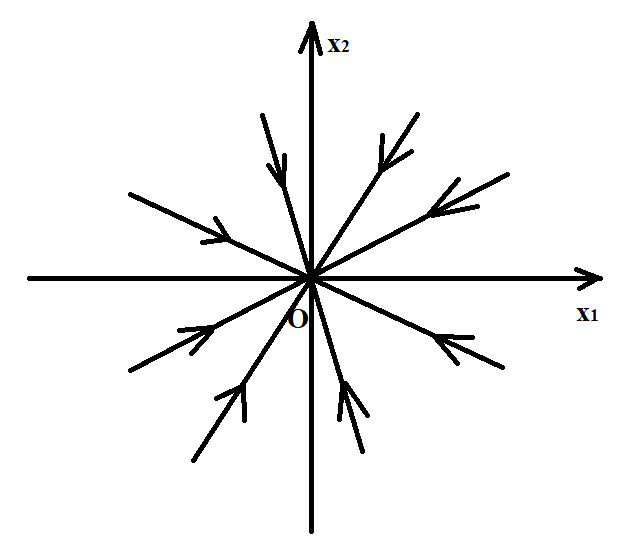
\includegraphics[scale=0.5]{images/dicrit_in.png}$$
А если $a>0$, то точка $(x_1(t); x_2(t))\underset{t\to+\infty}{\to}\infty$.
$$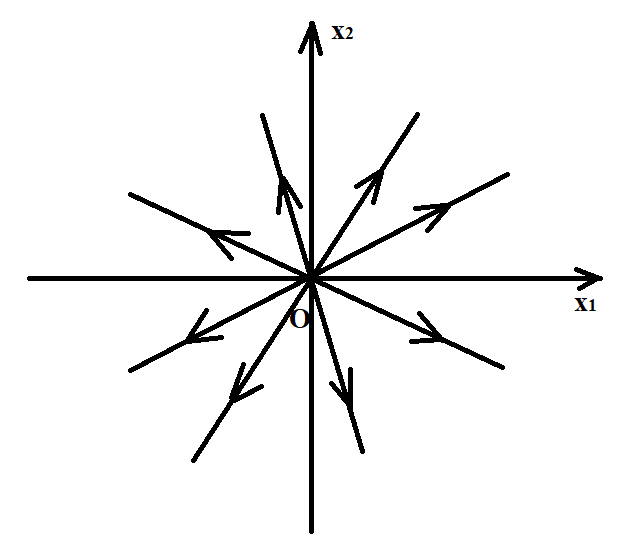
\includegraphics[scale=0.5]{images/dicrit_out.png}$$
\end{enumerate}
$\bullet$ \textit{Точка покоя, в окрестности которой фазовые графики имеют такое расположение, называется \textbf{дикритическим узлом} соответственно \textbf{устойчивым} и \textbf{неустойчивым}.}
\textbf{II группа.} Пусть матрица $A$ имеет вид $$A = \begin{pmatrix}
	a & b\\c & d
\end{pmatrix},$$ причем $A \ne aE$. Рассмотрим матрицу $$B = \begin{pmatrix}
0 & 1\\
-\det A & \Sp A
\end{pmatrix},\ \Sp A = a+d.$$ И рассмотрим их характеристические матрицы:
$$A - \lambda E = \begin{pmatrix}
	a - \lambda & b\\
	c & d-\lambda
\end{pmatrix},\quad B-\lambda E = \begin{pmatrix}
-\lambda & 1\\
-\det A & \Sp A - \lambda
\end{pmatrix}.$$
Построим для них системы НОД миноров.\\\\
$A - \lambda E$: $d_1(\lambda) = 1$ (если какое-то $c$ или $b$ не равно нулю, то оно является ненулевым минором первого порядка; а если $c = b = 0$, то $a\ne d$ и многочлены $a -\lambda$ и $d-\lambda$ взаимно простые).\\
$d_2(\lambda) = \lambda^2 - (a+d)\lambda + (ad - bc).$\\
$B - \lambda E$: $d_1(\lambda) = 1$, $d_2(\lambda) = \lambda^2 - \lambda\Sp A  + \det A.$\\\\
Следовательно, матрицы $A-\lambda E$ и $ B - \lambda E$ эквиваленты. Тогда матрицы $A$ и $B$ подобны, то есть существует невырожденная матрица $S$ такая, что $B = S^{-1}AS.$\\\\
Выполним замену в уравнении (3.8.1) неизвестной функции $X = SY$. Тогда $$SDY = ASY,$$ откуда, домножая на матрицу $S^{-1}$ слева, получим $$DY = S^{-1}ASY = BY.$$ То есть мы получили $$DY = BY.\eqno(3.8.2)$$
Координатная форма уравнения (3.8.2) имеет вид $$\begin{cases}
	Dy_1 = y_2,\\
	Dy_2 = -(\det A) y_1 + (\Sp A) y_2.
\end{cases}$$ Исключим из второго уравнения $y_1$ и получим $$D^2y_1 - (\Sp A)Dy_1 + (\det A)y_1 = 0.$$
Тогда решение $y_1(t)$ имеет фазовую траекторию, являющуюся графиком параметрически заданной функции $$\begin{cases}
	y_1 = y_1(t),\\
	y_2 = Dy_1(t);
\end{cases}\Rightarrow \begin{cases}
y_1 = y_1(t),\\
y_2 = y_2(t).
\end{cases}\eqno(3.8.3)$$ --- фазовая траектория решения уравнения (3.8.2).\\\\
То есть уравнение (3.8.3) и уравнение (3.8.2) имеют одинаковый фазовый портрет. Выполнив преобразование плоскости $X = SY$, получим фазовый портрет уравнения (3.8.1). Заметим, что матрица $S$ невырожденная. Тогда линейное преобразование $X = SY$ невырожденное. Следовательно, оно сводится к последовательному выполнению преобразования поворота и преобразования растяжения-сжатия вдоль двух взаимно перпендикулярных направлений. Таким образом, типы точек покоя уравнения (3.8.1) будут совпадать с типами точек покоя уравнений (3.8.2) и (3.8.3).
\chapter{Элементарные дифференциальные уравнения.}
\section{Дифференциальные уравнения первого порядка. Основные понятия.}
$\bullet$ \textit{\textbf{Дифференциальным уравнением первого порядка в нормальной форме} называется выражение вида $$P(x,y)dx + Q(x,y)dy = 0,\eqno(4.1.1)$$ где $P(x,y)$, $Q(x,y)$ --- функции, определенные в некоторой области $D\subseteq \Rm^2$.}\\\\
Если в области $D$ $Q(x,y) \ne 0$ $\forall (x,y)\in D$, то уравнение (4.1.1) можно представить в виде \begin{center}
	$\dfrac{dy}{dx} = f(x,y)$, где $f(x,y) = -\dfrac{P(x,y)}{Q(x,y)}$.
\end{center} 
$\bullet$ \textit{Уравнение в такой форме записи называется \textbf{разрешенным относительно производной}.}\\\\
Аналогично, если $P(x,y) \ne 0$ $\forall (x,y)\in D$, то уравнение (4.1.1) можно представить в виде \begin{center}
	$\dfrac{dx}{dy} = g(x,y)$, где $g(x,y) = -\dfrac{Q(x,y)}{P(x,y)}$.
\end{center} 
$\bullet$ \textit{Точка $(x_0,y_0) \in D$ такая, что $P(x_0,y_0) = Q(x_0,y_0) = 0$, называется \textbf{особой точкой} уравнения.}\\\\
$\bullet$ \textit{\textbf{Решением} уравнения называется функция $y(x)$ (или $x(y)$) определенная и дифференцируемая на некотором промежутке $\I \subseteq \Rm$, такая, что выполняется равенство $$P(x,y(x))dx + Q(x, y(x))\cdot y^\prime(x)dy = 0.$$}
$\bullet$ \textit{График решения дифференциального уравнения называется \textbf{интегральной кривой}.}\\\\
Решение уравнения может быть также задано или параметрически $$\begin{cases}
	x = x(t),\\
	y = y(t),
\end{cases} \quad t \in \I,$$ или неявно $\varphi(x,y) = 0$.\\\\
$\bullet$ \textit{\textbf{Общим решением} дифференциального уравнения называется семейство решений} \begin{enumerate}
	\item $y = y(x,C)$, $x = x(y,C)$, \textit{если решения заданы функциями};
	\item $\begin{cases}
		x = x(t,C),\\
		y = y(t,C).
	\end{cases}$ \textit{если решения заданы параметрически};
\item $\varphi(x,y,C) = 0$, \textit{если решения заданы неявно};
\end{enumerate}
\textit{зависящие от произвольной постоянной $C \in \Rm$.}\\\\
$\bullet$ \textit{Если в общем решении можно выразить произвольную постоянную $C$, то соотношение $$u(x,y) = C$$ называется \textbf{общим интегралом} уравнения.}\\\\
$\bullet$ \textit{Множество всех решений дифференциального уравнения называется \textbf{полным решением}.}
\section{Уравнения в полных дифференциалах. Уравнения с разделенными переменными.}
Рассмотрим дифференциальное уравнение в нормальной форме $$P(x,y)dx + Q(x,y)dy = 0,\quad (x,y)\in D\subseteq\Rm^2.\eqno(4.2.1)$$
Если Ф2П $u(x,y)$ дифференцируема по каждой переменной, то ее полный дифференциал имеет вид $$du(x,y) = u^\prime_x(x,y)dx + u^\prime_y(x,y)dy.$$
$\bullet$ \textit{Уравнение $(4.2.1)$ называется \textbf{уравнением в полных дифференциалах}, если его левая часть является полным дифференциалом некоторой функции $u(x,y)$, то есть $$du(x,y) = P(x,y)dx + Q(x,y)dy.$$ Это возможно тогда и только тогда, когда выполняется условие Эйлера $$\dfrac{\partial P}{\partial y} = \dfrac{\partial Q}{\partial x}.$$}
В этом случае уравнение (4.2.1) принимает вид $$du(x,y) = 0.$$
Следовательно, функция $u(x,y) = C$ является общим интегралом уравнения (4.2.1) и полным решением уравнения (4.2.1).\\\\
Любое $C$, для которого это равенство определено неявно, задает дифференцируемую функцию.\\\\
Найдем функцию $u(x,y)$. Если уравнение (4.2.1) является уравнением в полных дифференциалах, то $$\begin{dcases}
	\dfrac{\partial u}{\partial x} = P(x,y),\\
	\dfrac{\partial u}{\partial y} = Q(x,y).
\end{dcases}$$
И пусть $(x_0,y_0) \in D$. Тогда первое уравнение является простейшим относительно $x$. И, следовательно, $$u(x,y) = \int\limits^x_{x_0}P(x,y)dx + \varphi(y).$$
Продифференцируем это равенство по $y$. Тогда \begin{multline*}
	\dfrac{\partial u}{\partial y} = \int\limits^x_{x_0}\dfrac{\partial P}{\partial y}dx + \varphi^\prime(y) = \dfrac{\partial u}{\partial y} = \int\limits^x_{x_0}\dfrac{\partial Q}{\partial x}dx + \varphi^\prime(y) =\\= Q(x,y)\Big|_{x_0}^x + \varphi^\prime(y) = Q(x,y) - Q(x_0,y) + \varphi^\prime(y).
\end{multline*}
Тогда из второго уравнения системы $$Q(x,y) = Q(x,y) - Q(x_0,y) + \varphi^\prime(y).$$
$$\varphi^\prime(y) = Q(x_0,y).$$
$$\varphi(y) = \int\limits_{y_0}^y Q(x_0,y)dy + C.$$
Подставим обратно в $u(x,y)$ и получим $$u(x,y) =\int\limits^x_{x_0}P(x,y)dx  +  \int\limits_{y_0}^y Q(x_0,y)dy + C.$$
Выбрав одну из этих функций $u(x,y)$, например с $C = 0$, получим общий интеграл уравнения $$\int\limits^x_{x_0}P(x,y)dx  +  \int\limits_{y_0}^y Q(x_0,y)dy = C.$$
Если начать поиск функции $u(x,y)$ с интегрирования второго уравнения системы, то общий интеграл будет иметь вид $$\int\limits^x_{x_0}P(x,y_0)dx  +  \int\limits_{y_0}^y Q(x,y)dy = C.$$
Функция $u(x,y)$ может быть также найдена как КРИ-2: $$u(x,y) = \int\limits_{(x_0,y_0)}^{(x,y)}P(x,y)dx + Q(x,y) dy.$$
Задача Коши для уравнения в полных дифференциалах с начальными условиями $y|_{x=x_0} = y_0$ имеет решение $$\int\limits_{(x_0,y_0)}^{(x,y)}P(x,y)dx + Q(x,y) dy = 0,$$
если точка $(x_0,y_0)$ не является особой.\\\\
$\bullet$ \textit{Уравнение $$P(x)dx + Q(y)dy = 0$$ называется \textbf{уравнением с разделенными переменными}.}\\\\
Оно является уравнением в полных дифференциалах, так как $\dfrac{\d P}{\d y} = \dfrac{\d Q}{\d x} = 0$. Общий интеграл для него имеет вид $$\int\limits_{(x_0,y_0)}^{(x,y)}P(x)dx + Q(y) dy = C.$$
\section{Интегрирующий множитель. Уравнение с разделяющимися переменными.}
Рассмотрим уравнение в нормальной форме $$P(x,y) dx +Q(x,y) dy  =0,\quad (x,y)\in D.\eqno (4.3.1)$$
И пусть уравнение (4.3.1) не является уравнением в полных дифференциалах.\\\\
$\bullet$ \textit{Функция $\mu(x,y)$ называется \textbf{интегрирующим множителем} для уравнения $(4.3.1)$, если уравнение $$\mu(x,y)P(x,y)dx + \mu(x,y)Q(x,y)dy = 0\eqno (4.3.2)$$
является уравнением в полных дифференциалах.}\\\\
Заметим, что при домножении уравнения на функцию $\mu(x,y)$ полученное уравнение может либо приобрести дополнительные решения, либо потерять какие-либо решения. Так как уравнение (4.3.2) должно быть уравнением в полных дифференциалах, то функция $\mu(x,y)$ должна удовлетворять равенству $$\dfrac{\d \mu P}{\d y} = \dfrac{\d \mu Q}{\d x}\quad \Rightarrow\quad  \dfrac{\d \mu}{\d y}\cdot P + \mu\cdot \dfrac{\d P}{\d y} = \dfrac{\d \mu}{\d x}\cdot Q + \mu \cdot \dfrac{\d Q}{\d x}.$$
$$\mu(x,y)\cdot \Big(\dfrac{\d P}{\d y} - \dfrac{\d Q}{\d x}\Big) = \dfrac{\d \mu }{\d x}\cdot Q - \dfrac{\d \mu}{\d y}\cdot P.$$
Будем искать решение последнего уравнения в виде $\mu = \mu(\omega)$, где $\omega = \omega(x,y)$ --- некоторая функция. Тогда $$\mu(\omega)\cdot \Big(\dfrac{\d P}{\d y} - \dfrac{\d Q}{\d x}\Big) = \dfrac{\d \mu}{\d \omega}\cdot \dfrac{\d \omega}{\d x}\cdot Q - \dfrac{\d \mu}{\d \omega}\cdot \dfrac{\d \omega}{\d y}\cdot P.$$
Следовательно, $$\dfrac{\frac{\d \mu}{\d \omega}}{\mu (\omega)} = \dfrac{\dfrac{\d P}{\d y} - \dfrac{\d Q}{\d x}}{\dfrac{\d \omega}{\d x}\cdot Q - \dfrac{\d \omega}{\d y}\cdot P}.$$
$$(\ln \mu(\omega))'= -\dfrac{\dfrac{\d P}{\d y} - \dfrac{\d Q}{\d x}}{\dfrac{\d \omega}{\d y}\cdot P-\dfrac{\d \omega}{\d x}\cdot Q}.$$
Если функция справа является функцией от $\omega$, то есть имеет вид $\varphi(\omega)$, то $$(\ln \mu(\omega))' = \varphi(\omega).$$
Следовательно, отсюда
$$\ln \mu (\omega) = \int\limits_{\omega_0}^{\omega} \varphi(\tau)d\tau + C,$$
возводим все в степень $e$, тогда 
$$\mu(\omega) = e^{\int\limits_{\omega_0}^{\omega} \varphi(\tau)d\tau + C}.$$
В итоге получаем функцию
$$\mu(x,y) = e^{\int\limits_{\omega_0}^{\omega} \varphi(\tau)d\tau + C},$$
которая является интегрирующим множителем уравнения (4.3.1) для любого $C$.\\\\
$\bullet$ \textit{Уравнение вида $$P_1(x)P_2(y)dx + Q_1(x)Q_2(y)dy = 0$$ называется \textbf{уравнением с разделяющимися переменными}.}\\\\
Интегрирующий множитель этого уравнения имеет вид $$\mu(x,y) = \dfrac{1}{Q_1(x)P_2(y)},$$ так как в результате домножения получаем уравнение $$\dfrac{P_1(x)}{Q_1(x)}dx + \dfrac{Q_2(y)}{P_2(y)}dy = 0$$ --- уравнение с разделенными переменными.\\\\
Уравнение с разделяющимися переменными в виде разрешенном относительно производной имеет вид $$y' = f_1(x)\cdot f_2(y).$$
\section{Линейные уравнения. Уравнения Бернулли. Уравнения Риккати.}
Рассмотрим линейное уравнение первого порядка в нормальном виде $$(p(x)\cdot y + q(x))dx + r(x)dy = 0,\quad (x,y)\in D$$
или в виде разрешенном относительно производной $$y' = P(x)\cdot y + Q(x).$$
$$y' - P(x)\cdot y = Q(x).$$
Домножим уравнение так, чтобы свернуть в производную
$$y' - P(x)\cdot y = Q(x)\ \Big| \cdot e^{-\int\limits_{x_0}^xP(\tau)d\tau}.$$
$$y' \cdot e^{-\int\limits_{x_0}^xP(\tau)d\tau} - P(x)\cdot y\cdot e^{-\int\limits_{x_0}^xP(\tau)d\tau} = Q(x)\cdot e^{-\int\limits_{x_0}^xP(\tau)d\tau}.$$
$$\Big(y\cdot e^{-\int\limits_{x_0}^xP(\tau)d\tau}\Big)'= Q(x)\cdot e^{-\int\limits_{x_0}^xP(\tau)d\tau}.$$
$$y\cdot e^{-\int\limits_{x_0}^xP(\tau)d\tau} = \int\limits_{x_0}^x Q(t)\cdot e^{-\int\limits_{t_0}^tP(\tau)d\tau} dt + C.$$
Тогда формула
$$y = e^{\int\limits_{x_0}^xP(\tau)d\tau} \cdot \Big(C+\int\limits_{x_0}^x Q(t)\cdot e^{-\int\limits_{t_0}^tP(\tau)d\tau} dt\Big)$$ --- полное решение линейного уравнения первого порядка.\\\\
$\bullet$ \textit{\textbf{Уравнением Бернулли} называется уравнение вида} $$y' = P(x)\cdot y + Q(x)\cdot y^k,\quad k\in \Z\backslash\{0,1\}.$$
Разделим это уравнение на $y^k$. Получим $$\dfrac{y'}{y^k} = P(x)\cdot y^{1-k} + Q(x),$$
если $k>0$, можем потерять решение $y = 0$.\\\\
Выполним замену неизвестной функции $z(x) = y(x)^{1-k}$. Тогда $z' = (1-k)\cdot y^{-k}\cdot y'.$ Отсюда следует, что
$$\dfrac{y'}{y^k} = \dfrac{z'}{1-k}.$$
И, следовательно, $$\dfrac{z'}{1-k} = P(x)\cdot z + Q(x).$$
$$z' = (1-k)\cdot P(x)\cdot z + (1-k)\cdot Q(x)$$
--- линейное уравнение первого порядка.\\\\
Решив линейное уравнение и выполнив обратную замену, получим общее решение уравнения Бернулли (полное решение получим, добавив $y = 0$, если $k > 0$).\\\\
$\bullet$ \textit{\textbf{Уравнением Риккати} называется уравнение вида} $$y' = p(x)\cdot y^2 + q(x)\cdot y + r(x).\eqno (4.4.1)$$
Если $p(x) \equiv 0$, то (4.4.1) --- линейное уравнение. Если $r(x)\equiv 0 $, то (4.4.1) --- уравнение Бернулли. Пусть $p(x)\not\equiv 0$, $r(x)\not\equiv0$.\\\\
Уравнение Риккати в общем случае в квадратурах не интегрируется (то есть нельзя получить его решение в виде какого-то интеграла). Но в частных случаях уравнение может быть проинтегрировано:
\begin{enumerate}
	\item Если $p(x) = q(x) = r(x)$, то \begin{center}
		$\dfrac{dy}{dx} = p(x)\cdot (a_2y^2 +a_1y + a_0)$ --- уравнение с разделяющими переменными;
	\end{center} 
\item \begin{center}
	$y' = a_2\cdot \dfrac{y^2}{x^2} +a_1\cdot \dfrac{y}{x} + a_0$ --- однородное уравнение;
\end{center}
\end{enumerate}
Если известно хотя бы одно частное решение уравнения Риккати $y_1(x)$, то уравнение Риккати может быть приведено к линейному заменой неизвестной функции $y(x) = y_1(x) \pm \dfrac{1}{z(x)}$ или $z(x) = \dfrac{1}{y - y_1}$. При этом может быть потеряно решение $y = y_1$. Тогда $$y_1' - \dfrac{z'}{z^2} = p(x)\cdot \Big(y_1^2 + 2\cdot\dfrac{y_1}{z} + \dfrac{1}{z^2}\Big) + q(x)\cdot\Big(y_1 + \dfrac{1}{z}\Big) +r(x).$$
Так как $y_1$ является решением уравнения Риккати, то $$y_1' = p(x)\cdot y_1^2 + q(x)\cdot y_1 + r(x).$$
Следовательно, $$-\dfrac{z'}{z^2} = p(x)\cdot \dfrac{2y_1}{z} + \dfrac{p(x)}{z^2} + q(x)\cdot \dfrac{1}{z} \quad \Big|\quad \cdot (-z^2).$$
\begin{center}
	$z' = (-p(x)\cdot 2 y_1 - q(x))\cdot z - p(x)$ --- линейное уравнение.
\end{center}
$\bullet$ \textit{Уравнение Риккати называется \textbf{каноническим}, если оно имеет вид} $$y' = \pm y^2 + R(x).$$
Уравнение Риккати может быть приведено к каноническому виду заменой неизвестной функции вида $$y = \alpha (x)\cdot z (x) + \beta (x),$$
где $z(x)$ --- новая неизвестная функция. Найдем $\alpha(x)$ и $\beta (x)$. Подставим замену и получим
$$\alpha ' z + \alpha z' + \beta' = p(\alpha ^2 z^2 + \beta ^2 + 2\alpha \beta z) + q(\alpha z + \beta ) + r.$$
$$\alpha z' = p\alpha^2z^2 + z(2p\alpha\beta + q\alpha - \alpha') + p\beta^2 + q\beta + r - \beta'.$$
$$z' = p\alpha z^2 + \Big(2p\beta + q - \dfrac{\alpha '}{\alpha }\Big)z + \dfrac{1}{\alpha} (p\beta^2 + q\beta + r - \beta ^2).$$
Подберем функции $\alpha(x)$ и $\beta (x)$ так, чтобы $$p\alpha = \pm 1\Rightarrow \alpha = \pm \dfrac{1}{p};$$
$$2p\beta + q -\dfrac{\alpha '}{\alpha } = 0\Rightarrow\beta = \dfrac{1}{2p}\Big(\dfrac{\alpha '}{\alpha} - q\Big).$$
\section{Однородные уравнения.}
	$\bullet$ \textit{Функция двух переменных $F(x,y)$ называется \textbf{однородной функцией степени} $k$, если $F(tx,ty) = t^kF(x,y)$.}\\\\
	$\bullet$ \textit{Уравнение $$P(x,y)dx + Q(x,y)dy = 0$$ называется \textbf{однородным уравнением}, если функции $P(x,y)$ и $Q(x,y)$ являются однородными функциями одной степени.}\\\\
	Если однородное уравнение представить в виде разрешенном относительно производной, то получим $$\dfrac{dy}{dx} = -\dfrac{P(x,y)}{Q(x,y)}.$$
	При этом $$\dfrac{P(tx,ty)}{Q(tx,ty)} = \dfrac{t^kP(x,y)}{t^kQ(x,y)} = \dfrac{P(x,y)}{Q(x,y)}.$$
	Следовательно, эта функция также является однородной функцией степени 0. Любая однородная функция степени 0 представима в виде $$F(x,y) = F\Big(x,x\cdot \dfrac{y}{x}\Big) = x^0F\Big(1, \dfrac{y}{x}\Big) =F\Big(1,\dfrac{y}{x}\Big) = f\Big(\dfrac{y}{x}\Big).$$
	Следовательно, однородное уравнение имеет вид $$y' = f\Big(\dfrac{y}{x}\Big).$$
	Выполнив замену независимой переменной $$z(x) = \dfrac{y(x)}{x}\text{, или }y(x) = x\cdot z(x),$$ получим $$z(x) + xz' = f(z).$$
	Тогда \begin{center}
		$x\dfrac{dz}{dx} = f(z) - z$ --- уравнение с разделяющимися переменными.
	\end{center}
	$$\dfrac{dz}{f(z) - z} = \dfrac{dx}{x}.$$
	Заметим, что могут быть потеряны решения вида $f(z) - z = 0$ либо приобретены решения вида $$\dfrac{1}{f(z) - z} = 0.$$
	Если однородное уравнение задано в нормальной форме, то, выполнив замену $$y(x) = x\cdot z(x),$$ получим $$P(x,xz)dx + Q(x,xz) (xdz + zdx) = 0.$$
	$$(\underbrace{P(x,xz)}_{x^kP(1,z)} + z\cdot \underbrace{Q(x,xz)}_{x^kQ(1,z)})dx +x\cdot  \underbrace{Q(x,xz)}_{x^kQ(1,z)}dz = 0.$$
	$$(\underbrace{P(1,z) + z\cdot Q(1,z)}_{f_1(z)})dx + \underbrace{Q(1,z)}_{f_2(z)}\cdot \underbrace{x}_{g_1(x)}\cdot dz = 0.$$
	Получили уравнение с разделяющимися переменными.\\\\
Рассмотрим уравнение  $$y' = f\Big(\dfrac{a_1x + b_1y + c_1}{a_2 x + b_2y + c_2}\Big).$$
\begin{enumerate}
	\item Пусть $\dfrac{a_1}{a_2} = \dfrac{b_1}{b_2}$. Тогда $a_1x + b_1y = k(a_2x + b_2y)$. Тогда уравнение имеет вид $$y' = g(ax + by).$$
	Выполним замену неизвестной функции $$ax + by(x) = z(x)\Rightarrow y = \dfrac{1}{b}(z-ax).$$
	$$\dfrac{1}{b}(z' - a) = g(z).$$
	\begin{center}
		$ z' = bg(z) + a$ --- уравнение с разделяющимися переменными.
	\end{center}
\item Пусть $\dfrac{a_1}{a_2}\ne \dfrac{b_1}{b_2}$. Выполним замену $$\begin{cases}
	x = t + \alpha,\\
	y = z + \beta,
\end{cases}$$
где $t$ --- новая независимая переменная, $z$ --- новая неизвестная функция, зависящая от $t$, а $\alpha,\beta \in \Rm$. Тогда $$\dfrac{dy}{dx} = \dfrac{dz}{dt}\Rightarrow y' = f\Big(\dfrac{a_1(t+\alpha) + b_1(z+\beta) + c_1}{a_2(t+\alpha) + b_2(z+\beta) + c_2}\Big).$$
Подберем свободные константы так, чтобы $$\begin{cases}
	a_1\alpha + b_1\beta + c_1 = 0,\\
	a_2\alpha + b_2\beta + c_2 = 0.
\end{cases}$$
Так как $\dfrac{a_1}{a_2}\ne \dfrac{b_1}{b_2}$, то $\begin{vmatrix}
	a_1&b_1\\
	a_2&b_2
\end{vmatrix}\ne 0$, и система невырожденная и имеет единственное решение. Следовательно, уравнение имеет вид $$z' = f\Big(\dfrac{a_1 t + b_1 z}{a_2 t + b_2 z}\Big),$$
причем $$f\Big(\dfrac{a_1 t + b_1 z}{a_2 t + b_2 z}\Big) = f\Big(\dfrac{t(a_1  + b_1 \frac{z}{t})}{t(a_2  + b_2 \frac{z}{t})}\Big) = f\Big(\dfrac{a_1  + b_1 \frac{z}{t}}{a_2  + b_2 \frac{z}{t}}\Big) = g\Big(\dfrac{z}{t}\Big).$$
То есть уравнение имеет вид \begin{center}
	$z' = g\Big(\dfrac{z}{t}\Big)$ --- однородное уравнение.
\end{center}
\end{enumerate}
\section {Существование и единственность решения задачи Коши.}
Рассмотрим задачу Коши $$\begin{cases}
	y' = f(x,y),\ (x,y)\in D\subseteq \Rm^2,\\
	y(x_0) = y_0,\ (x_0,y_0)\in D;
\end{cases}\eqno (4.6.1)$$
где $f(x,y)$ --- непрерывная в $D$ функция.
\begin{lem}
	[интегральный признак]
	Непрерывная функция $y:\I \to \Rm$, где $\I$ --- некоторый промежуток, является решением задачи Коши $(4.6.1)$ $\Longleftrightarrow$ она удовлетворяет следующему условию $$y(x) = y_ 0 +\int\limits_{x_0}^x f(\tau, y(\tau))d\tau, \quad x_0,x\in \I.$$
\end{lem}\begin{Proof}
$\Rightarrow)$ Так как $y(x)$ --- решение задачи Коши (4.6.1), то $$y'(x) = f(x,y(x)).$$ Проинтегрируем это равенство $$\intx y'(x)dx = \intx f(\tau,y(\tau))d\tau,$$
$$y(x)\Big|_{x_0}^x = \intx f(\tau,y(\tau))d\tau.$$
$\Leftarrow)$ Так как функции $y(x)$ и $f(x,y)$ непрерывные, то функция $f(x,y(x))$ также непрерывная как композиция непрерывных функций. Следовательно, правая часть интегрального уравнения --- дифференцируемая функция, а тогда функция $y(x)$ также дифференцируема. Продифференцируем это уравнение $$y'(x) = f(x,y(x)).$$ Тогда $y(x_0) = y_0$ --- решение задачи Коши.
\end{Proof}
\begin{theorem}
	[Пикара-Линделефа]
	Если функция $f(x,y)$ непрерывна в некоторой области $D\subseteq\Rm^2$ и в некоторой окрестности содержащейся в $D$ удовлетворяет условию Липшица, то есть $$\exists L:\forall (x,y_1),(x,y_2)\in U\quad |f(x,y_1) - f(x,y_2)| \leq L|y_1 - y_2|,$$
	то задача Коши $(4.6.1)$ имеет единственное решение, которое может быть найдено методом последовательных приближений:
		$$y(x) = \lim\limits_{n\to\infty}y_n(x),\ \text{где}\ y_0(x) = y_0,\ y_n(x) = y_0 + \intx f(\tau,y_{n-1}(\tau))d\tau,\ n = 1,2,\ldots$$
\end{theorem}
\begin{Proof}
	\begin{enumerate}
		\item Существование.\\\\
		Рассмотрим прямоугольник $$\Pi = \{(x,y)\ \big|\
			|x-x_0|\leq a,
			|y-y_0|\leq a \},$$
			который целиком содержится в области $U$. Так как функция $f$ в прямоугольнике $\Pi$ непрерывна, то она ограничена. \\\\Пусть $|f(x,y)|\leq M$, $\forall(x,y)\in \Pi$. Покажем, что если $\delta = \min\{a, \frac{a}{M}\}$, то $\forall \I = [x_0 - \delta, x_0 + \delta]$ функция $y_n(x)$ содержится в $\Pi$.
			\begin{multline*}
				|y_1(x) - y_0(x)| = \Big|\intx f(\tau, y_0)d\tau\Big|\leq \Big|\intx |f(\tau, y_0)|d\tau\Big|\leq \Big|\intx Md\tau\Big| =\\= |M\cdot (x-x_0)| = M\cdot |x-x_0|\leq M\cdot \delta\leq M\cdot \dfrac{a}{M} = a.
			\end{multline*}
		То есть точка $(x,y_1(x))\in \Pi$ $\forall x \in \I$.
		$$
		|y_2(x) - y_0(x)| = \Big|\intx f(\tau, y_1)d\tau\Big|\leq \Big|\intx |f(\tau, y_1)|d\tau\Big|\leq \Big|\intx Md\tau\Big| \leq a.
		$$
		Аналогично рассуждая, получим, что $|y_n(x) - y_0|\leq a $, то есть точки $(x,y_n(x))\in \Pi$ $\forall x \in \I$.\\\\
		Покажем, что $\forall x \in \I$ $\exists \lim\limits_{n\to \infty} y_n(x) = y(x)$. Заметим, что $$y_n(x) = y_0 + (y_1(x) - y_0) + (y_2(x) - y_1(x)) +\ldots + (y_n(x) - y_{n-1}(x)).$$
		Следовательно, функция $y_n(x)$ является частичной суммой ряда $$y_0 + \sum_{i=1}^{\infty}(y_i - y_{i-1}).\eqno (4.6.2)$$
		Докажем сходимость этого ряда по признаку Вейерштрасса, для этого найдем мажорирующую константу.
		$$|y_1(x) - y_0(x)| \leq \Big|\intx |f(\tau, y_0)d|\tau\Big|\leq M\cdot |x-x_0|.$$
		\begin{multline*}
			|y_2(x) - y_1(x)| \leq \Big|\intx \big|f(\tau, y_1(\tau))d\tau - \intx f(\tau, y_0(\tau))\big|d\tau\Big|\leq \Big|\intx L|y_1(\tau) - y_0(\tau)|d\tau\Big|\leq\\\leq \Big|\intx LM(\tau - x_0)d\tau\Big| = LM\dfrac{(\tau - x_0)^2}{2}\Big|_{x_0}^x = LM\dfrac{(x - x_0)^2}{2}.
		\end{multline*}
				\begin{multline*}
					|y_3(x) - y_2(x)| \leq \Big|\intx \big|f(\tau, y_2(\tau))d\tau - \intx f(\tau, y_1(\tau))\big|d\tau\Big|\leq \Big|\intx L|y_2(\tau) - y_1(\tau)|d\tau\Big|\leq\\\leq \Big|\intx L^2M\dfrac{(\tau - x_0)^2}{2}d\tau\Big| = L^2M\dfrac{(\tau - x_0)^3}{2\cdot 3}\Big|_{x_0}^x = L^2M\dfrac{(x - x_0)^3}{3!}.
				\end{multline*}
			Продолжая рассуждать аналогично, получим что $$|y_i(x) - y_{i-1}(x)|\leq L^{i-1}M\dfrac{|x - x_0|^i}{i!}.$$
			Следовательно, ряд $y_0 + \sum_{i=1}^{\infty}(y_i - y_{i-1})$ мажорируется числовым рядом
			$$|y_0| + \sum_{i=1}^{\infty}L^{i-1}M\dfrac{|x - x_0|^i}{i!} = [|x-x_0|\leq\delta] \leq |y_0| + \dfrac{M}{L}\cdot\sum_{i=1}^{\infty}\dfrac{(L\delta)^i}{i!} = |y_0|+\dfrac{M}{L}\cdot (e^{L\delta} - 1).$$
			То есть ряд (4.6.2) по признаку Вейерштрасса сходится равномерно, значит $\exists \lim\limits_{n\to \infty}y_n(x)$. \\\\
			Покажем, что построенная функция является решением задачи Коши (4.6.1). Так как последовательность $y_n(x)\rightrightarrows y(x)$, а функция $f$ удовлетворяет условию Липшица, то последовательность $f(x,y_n(x))\rightrightarrows f(x,y(x))$, то есть
			$$\lim\limits_{n\to \infty}f(x,y_n(x)) = f(x, \lim\limits_{n\to\infty} y_n(x)) = f(x,y(x)).$$
			И, следовательно, \begin{multline*}
				y(x) = \lim\limits_{n\to \infty} y_n = \lim\limits_{n\to \infty}\Big(y_0 + \intx f(\tau, y_{n-1}(\tau))d\tau\Big) =\\= y_0 + \lim\limits_{n\to \infty}\intx f(\tau, y_{n-1}(\tau))d\tau = y_0 + \intx f(\tau, y(\tau))d\tau.
			\end{multline*}
		Следовательно, по интегральному признаку функция $y(x)$ --- решение задачи Коши.
		\item Единственность.\\\\
		Пусть задача Коши имеет 2 различных решения $z(x)$, $y(x)$, то есть в любой окрестности точки $x_0$ $\exists\epsilon : z(\epsilon)\ne y(\epsilon)$.\\\\
		Пусть $x > x_0$. Тогда\begin{multline*}
			|y(x) - z(x)| = \Big|\intx \big(f(\tau,y(\tau)) - f(\tau,z(\tau))\big)d\tau\Big|\leq \Big| \intx \big|f(\tau,y(\tau)) - f(\tau,z(\tau))\big|d\tau\Big| \leq \\ \leq  \Big|\intx L \big|y(\tau) -z(\tau)\big|d\tau\Big| \leq \intx L \big|y(\tau) -z(\tau)\big|d\tau;
		\end{multline*}
		$$\underbrace{|y(x)-z(x)|}_{\varphi'(x)} - \underbrace{\Big|\intx L \big|y(\tau) -z(\tau)\big|d\tau\Big|}_{\varphi(x)} \leq 0.$$
		$$\varphi'(x) - L\varphi(x) \leq 0.$$
		Домножим неравенство на $e^{-Lx}$. Тогда
			$$\varphi'(x)\cdot e^{-Lx} - L\varphi(x)\cdot  e^{-Lx} \leq 0.$$
			$$D(\varphi(x)\cdot e^{-Lx})\leq 0.$$
			Следовательно, функция $\varphi(x)\cdot e^{Lx}$ не возрастает на отрезке $[x_0;x]$. Поэтому $$\varphi(x)\cdot e^{-Lx} \leq \varphi(x_0)\cdot  e^{-Lx_0}\leq0.$$ Но так как подынтегральная функция $\varphi(x)$ неотрицательна и $x > x_0$, то $\varphi(x)\cdot~e^{-Lx}\geq~0$. И, следовательно, $\varphi(x)\cdot e^{-Lx} = 0$, то есть $\varphi(x) = |y(x) - z(x)| = 0$. Отсюда следует, что $y(x) = z(x)$.
			\end{enumerate}
\end{Proof}
\begin{theorem}
	[Пеано]
	Если функция $f(x,y)$ непрерывна в области $D$, то задача Коши $(4.6.1)$ имеет по крайней мере одно решение $y(x)$ на некотором промежутке $I = [ x_0 - \delta; x_0 + \delta]$.
\end{theorem}
\begin{Proof}
	Без доказательства.
\end{Proof}
\begin{theorem}
	[об условии Липшица]
	Если на некотором замкнутом ограниченном множестве $U\subseteq \Rm^2$ функция $f(x,y)$ непрерывна вместе со своей частной производной $f'_y$, то функция $f(x,y)$ удовлетворяет условию Липшица по $y$.
\end{theorem}
\begin{Proof}
		Так как функция $f(x,y)$ дифференцируема по $y$, то по теореме Лагранжа $$\exists \xi: |f(x,y_1) - f(x,y_2)| = f'_y(x,\xi)\cdot |y_1 - y_2|.$$ И так как множество $U$ замкнуто и ограничено и $f(x,y)$ непрерывна на $U$, то непрерывная функция $f'_y(x,y)$ ограничена. Следовательно, $\exists L : |f'_y(x,\xi)| \leq L \Rightarrow$ $$|f(x,y_1) - f(x,y_2)| \leq L|y_1 - y_2|.$$
		Что и является условием Липшица.
\end{Proof}
\section{Особые решения.}
Рассмотрим дифференциальное уравнения $$P(x,y)dx + Q(x,y)dy = 0 \quad (x,y) \in D \subseteq \Rm^2.\eqno(4.7.1)$$
$\bullet$ \textit{Точка $M(x,y)$ --- \textbf{точка существования} для уравнения $(4.7.1)$, если через нее проходит хотя бы одна интегральная кривая уравнения $(4.7.1)$, то есть график решения.}\\\\
$\bullet$ \textit{Точка существования, обладающая окрестностью, внутри которой все интегральные кривые, проходящие через эту точку, совпадают, называется \textbf{точкой единственности}.}\\\\
$\bullet$ \textit{Точка существования, через которую проходят две интегральные кривые с одной касательной в этой точке, отличающиеся в любой окрестности этой точки, называется \textbf{точкой ветвления}.}\\\\
$\bullet$ \textit{Решение, каждая точка которого является точкой ветвления, называется\textbf{ особым решением}.}\\\\
\textbf{Замечание.} Если уравнение имеет особое решение, то кроме него и частных решений, входящих в общее решение уравнение будет иметь \textbf{составные решения}, построенные из частей частных и особых решений.\\\\
Для поиска особых решений уравнения $(4.7.1)$ могут использоваться два подхода.\\\\
\textbf{I подход.}
Функции, подозрительные на особые решения для уравнения $y' = f(x,y)$ могут быть найдены из теоремы о существовании и единственности задачи Коши, так как графики особых решений состоят из точек ветвлений, а значит, в каждой его точке нарушается теорема о существовании и единственности, а единственность нарушается в случае невыполнения условия Липшица. В частности, функциями, подозрительными на особые решения, могу быть функции, вдоль которых функция $f'_y(x,y)$ не определена.\\\\
\textbf{II подход.}
Особое решение может быть найдено, если известно общее решение. Пусть общее решение уравнения $(4.7.1)$ имеет вид $$F(x,y,C) = 0. \eqno(4.7.2)$$ Это уравнение задает на плоскости однопараметрическое семейство интегральных кривых.\\\\
$\bullet$ \textit{Линия $\Gamma$ называется \textbf{огибающей} однопараметрического семейства линий, если она в каждой своей точке касается одной из линий семейства и ни на каком участке не совпадает с этой линией.}\\\\
Таким образом, огибающая семейства решений является особым решением уравнения, так как в каждой своей точке имеет касательную, совпадающую с касательной одного из решений семейства.
Огибающая семейства функций $(4.7.2)$ может быть найдена следующим образом. Если $\Gamma$ --- огибающая семейства $(4.7.2)$, то в каждой своей точке $(x_0,y_0) \in \Gamma$ она касается линии $\Gamma_{C_0}$, которая получается из уравнения $(4.7.2)$ при $C = C_0$.\\\\
Если аналогично поступить с каждой точкой линии $\Gamma$, получим параметрическое уравнение огибающей. $$\begin{cases}
	x = \varphi(C), \\
	y = \psi(C);
\end{cases}
$$ где $C$ --- параметр.
Причем $$F(\varphi(C), \psi(C), C) = 0.$$
Если функция $F(x, y, C)$ является дифференцируемой по каждой из своих переменных, то продифференцируем последнее равенство по $C$. Тогда $$\underbrace{F'_x(\varphi(C), \psi(C), C)\cdot \varphi'(C) + F'_y(\varphi(C), \psi(C), C)\cdot \psi'(C)}_{A} + F'_C(\varphi(C), \psi(C), C) = 0.$$
Покажем, что $A = 0.$ Пусть $F'^2_x + F'^2_y \ne 0.$ Найдем угловые коэффициенты касательных к линиям $\Gamma$ и $\Gamma_{C_0}$ в точке $(\varphi(C), \psi(C))$.\\\\
Найдем для $\Gamma$:
$$y' = \frac{\psi'(C)}{\varphi'(C)}.$$
Найдем для $\Gamma_{C_0}$. Неявное задание этой функции имеет вид $F(x, y, C) = 0$, следовательно получим:
$$F'_x + F'_y\cdot y' = 0.$$
Отсюда $$y' = -\dfrac{F'_x}{F'_y}.$$
Так как эти угловые коэффициенты равны, то
$$ \frac{\psi'(C)}{\varphi'(C)} = -\frac{F'_x(\varphi(C), \psi(C), C)}{F'_y(\varphi(C), \psi(C), C)}.$$
Приводя к общему знаменателю, получаем, что $A = 0$, следовательно, $F'_C = 0$.\\
Таким образом, точки, лежащие на огибающей, удовлетворяют системе
$$\begin{cases}
	F(x, y, C) = 0,\\
	F'_C(x, y, C)  = 0;
\end{cases} \eqno(4.7.3)$$
$\bullet$\textit{ Функции, точки которой удовлетворяют системе $(4.7.3)$, называются \textbf{дискриминантными кривыми} семейства $(4.7.2)$.
Если на дискриминантных кривых нет точек, для которых $F'^2_x + F'^2_y = 0$, то эта дискриминантная кривая является огибающей.}
\section{Уравнения 1-го порядка, не разрешенные относительно производной.}
Рассмотрим уравнение 1-го порядка $$F(x, y, y') = 0 \eqno(4.8.1),$$ и пусть функция $F$ непрерывна по всем своим аргументам в некоторой области $D \subseteq \Rm^3$. Если это уравнение можно разрешить относительно $y'$, то из $(4.8.1)$ можно получить одно или несколько уравнений вида $y' = f_i(x, y)$. Интегрируя эти уравнения, получим одно или несколько семейств решений исходного уравнения. Но кроме них уравнение $(4.8.1)$ может иметь составные решения, не являющиеся решениями ни одного из полученных уравнений. Это происходит, когда некоторая интегральная кривая одного уравнения касается в некоторой точке интегральной кривой другого уравнения.\\\\
Отсутствие составных решений  гарантируется отсутствием точек ветвления, а отсутствие точек ветвления означает единственность решения расширенной задачи Коши для $(4.8.1)$.
$$ F(x, y, y') = 0, \quad y|_{x=x_0} = y_0, \quad y'|_{x=x_0} = y_1 \eqno(4.8.2)$$
\begin{theorem}[о существовании и единственности решения расширенной задачи Коши]
	Если в некоторой замкнутой окрестности точки $(x_0, y_0, p_0) \in \Rm^3$ функция $F(x, y, p)$ удовлетворяет следующим условиям:
	\begin{enumerate}
		\item $F(x_0, y_0, p_0) = 0;$
		\item $\exists \dfrac{\d F}{\d p}(x_0, y_0, p_0) \ne 0.$
	\end{enumerate} 
	Тогда решение задачи Коши $(4.8.2)$ имеет единственное решение.
\end{theorem}
\begin{Proof}
	Если выполняются условия теоремы, то по теореме о неявной функции в окрестности точки $(x_0, y_0, p_0)$ уравнение $(4.8.1)$ задает однозначную функцию $y' = f(x, y)$, которая непрерывно дифференцируема в окрестности точки $(x_0, y_0)$, и при этом $f(x_0, y_0) = p_0.$ По теореме Пикара-Линделёфа для полученного уравнения решение задачи Коши существует и единственно.
\end{Proof}\\\\
$\bullet$ \textit{Множество точек $(x_0, y_0)$, в которых нарушается единственность решения расширенной задачи Коши, называется \textbf{особым множеством} для уравнения $(4.8.1)$.}\\\\
$\bullet$ \textit{Если график какой-либо функции $y = \varphi(x)$ лежит в особом множестве и при этом является интегральной кривой, то функция $y = \varphi(x)$ называется \textbf{особым решением}.}\\\\
Таким образом, особые решения удовлетворяют системе:
$$\begin{cases}
	F(x, y, p) = 0,\\
	F'_p(x, y, p) = 0.
\end{cases}$$
Исключим $p$ и получим функции, подозрительные на особые решения.
\subsection{Метод введения параметра.}
Пусть уравнение $(4.8.1)$ допускает параметрическое представление, то есть существуют функции
$$\begin{cases}
	x = \varphi(u, v),\\
	y = \psi(u, v),\\
	y' = \xi(u, v);
\end{cases}$$ такие, что $$F(\varphi(u, v), \psi(u, v), \xi(u, v)) \equiv 0.$$
Тогда $$y' = \frac{dy}{dx} = \xi(u, v) = \frac{\psi'_u du + \psi'_v dv}{\varphi'_u du + \varphi'_v dv}.$$
Следовательно, $$(\psi'_u - \varphi'_u\xi)du + (\psi'_v - \varphi'_v\xi)dv = 0.$$
Это обыкновенное дифференциальное уравнение в нормальной форме.\\\\
Если $v = v(u)$ --- решение этого дифференциального уравнения, то 
$$\begin{cases}
	x = \varphi(u, v(u)),\\
	y = \psi(u, v(u));
\end{cases}$$ --- решение исходного уравнения $(4.8.1)$.
\subsubsection{Уравнения, разрешенные относительно $x$ и $y$.}
\begin{enumerate}
	\item\textit{ Уравнения, разрешённые относительно $y$}.\\\\
	Пусть уравнение $(4.8.1)$ сводится к $y = f(x, y')$. Это уравнение допускает параметризацию вида:
	$$\begin{cases}
		x = u,\\
		y = f(u, v),\\
		y' = v;
	\end{cases}$$ или в более традиционной форме
	$$\begin{cases}
	x = x,\\
	y = f(x, p),\\
	y' = p.
\end{cases}$$
Из $y' = p$ следует, что
$$\frac{f'_xdx + f'_pdp}{dx} = p$$
$$(f'_x - p)dx + f'_pdp = 0$$
Если общее решение имеет вид $x = \varphi(p, C)$, то общее решение уравнения $(4.8.1)$ имеет параметрическое задание $$\begin{cases}
	x = \varphi(p, C),\\
	y = f(\varphi(p, C), p);
\end{cases}$$ где $p$ --- параметр.\\\\
Если же общее решение последнего уравнения имеет вид $p = \varphi(x, C)$, то общее решение $(4.8.1)$ задано явно $$y = f(x, \varphi(x, C)).$$
	\item\textit{ Уравнения, разрешенные относительно $x$.}\\\\
	Пусть уравнение $(4.8.1)$ сводится к $x = f(y, y')$. Это уравнение допускает параметризацию вида:
	$$\begin{cases}
		x = f(u, v),\\
		y = u,\\
		y' = v;
	\end{cases}$$ или в более традиционной форме
	$$\begin{cases}
		x = f(y, p),\\
		y = y,\\
		y' = p.
	\end{cases}$$
	Из $y' = p$ следует, что
	$$\frac{dy}{f'_ydy + f'_pdp} = p$$
	$$(1 - f'_yp)dy - pf'_pdp = 0$$
	Если общее решение имеет вид $y = \varphi(p, C)$, то общее решение уравнения $(4.8.1)$ имеет параметрическое задание $$\begin{cases}
		x = f(\varphi(p, C), p),\\
		y =  \varphi(p, C);
	\end{cases}$$ где $p$ --- параметр.\\\\
	Если же общее решение последнего уравнения имеет вид $p = \varphi(y, C)$, то общее решение $(4.8.1)$ задано явно $$x = f(y, \varphi(y, C)).$$
\end{enumerate}
\subsubsection{Уравнение Клеро.}
$\bullet$ \textit{Уравнение вида $$y = xy' + g(y')$$ называется \textbf{уравнением Клеро}.}\\\\
Введем параметризацию $$\begin{cases}
	x = x,\\
	y = xp + g(p),\\
	y' = p;
\end{cases}$$
Отсюда $dy = pdx$, $dy = pdx + (x + g'(p))dp.$ Тогда $$pdx = pdx + (x + g'(p))dp \Rightarrow (x + g'(p))dp = 0.$$
Рассмотрим 2 случая.\begin{enumerate}
	\item $dp = 0$. Тогда $p = C$. Отсюда \begin{center}
		$y = xC + g(C)$ --- общее решение.
	\end{center}
\item $x + g'(p) = 0.$ Тогда \begin{center}
	$\begin{cases}
		x = -g'(p),\\
		y = -g'(p)\cdot p + g(p);
	\end{cases}$ --- особое решение.
\end{center}
Найдем дискриминантные кривые семейства линий $y = xC + g(C)$:
$$\begin{cases}
	y = xC + g(C),\\
	0 = x + g'(C);
\end{cases}$$
Следовательно, найденное решение --- дискриминантная кривая $$\underbrace{y - xC - g(C)}_{\varphi} = 0.$$
$\varphi_y = 1$, отсюда особых точек семейство линий не имеет, следовательно, найденная дискриминантная кривая является огибающей.
\end{enumerate}
\subsubsection{Уравнение Лагранжа.}
$\bullet$ \textit{Уравнение вида $$y = x\cdot f(y') + g(y'),\quad f(y) \not\equiv y'$$ называется \textbf{уравнением Лагранжа}.}\\\\
Введем параметризацию $$\begin{cases}
	x = x,\\
	y = xf(p) + g(p),\\
	y' = p;
\end{cases}$$
Отсюда $dy = pdx$, $dy = f(p)dx + (xf' + g')dp.$ Тогда $$pdx = f(p)dx + (xf' + g')dp.$$
$$\underbrace{(p-f(p))}_{\not\equiv 0}dx = (xf' + g')dp.$$
Таким образом, получаем \begin{center}
	$\dfrac{dx}{dp} = \dfrac{xf' + g'}{p - f(p)}$ --- линейное уравнение относительно $x$.
\end{center}
Находя общее решение $x = \varphi(p,C)$, подставляем его в $y = xf(p) + g(p)$ и получим параметрически заданное решение исходного уравнения $$\begin{cases}
	x = \varphi(p,C),\\
	y = \varphi(p,C)\cdot f(p) + g(p).
\end{cases}$$
Причем, если $\exists \alpha \in \Rm : \alpha - f(\alpha ) = 0$, то уравнение Лагранжа имеет также решение $$y = x\cdot f(\alpha) + g(\alpha).$$
\subsubsection{Неполные уравнения.}
\begin{enumerate}
	\item Уравнение вида $F(x,y') = 0$. Если данное уравнение допускает параметризацию вида $$\begin{cases}
		x = \varphi(t),\\
		y' = \psi(t);
	\end{cases}$$
то есть $\exists \varphi(t), \psi(t) : F(\varphi(t),\psi(t)) = 0$.\\\\
Тогда $$dy = \psi(t)dx \Rightarrow dy = \psi(t)\varphi'(t)dt.$$
Получили уравнение с разделяющимися переменными. Следовательно, $$y = \int\limits_{t_0}^t \psi(\tau)\varphi'(\tau) d\tau + C.$$
Тогда общее решение имеет вид 
$$\begin{dcases}
	x = \varphi(t),\\
	y = \int\limits_{t_0}^t \psi(\tau)\varphi'(\tau) d\tau + C.
\end{dcases}$$
\item Уравнение вида $F(y,y') = 0$. Если данное уравнение допускает параметризацию вида
$$\begin{cases}
	y = \varphi(t),\\
	y' = \psi(t);
\end{cases}$$ то из равенства $dy = \psi(t)dx$ получаем уравнение с разделяющимися переменными $$\varphi'(t)dt =\psi(t)dx. $$
Тогда $$dx = \dfrac{\varphi'(t)}{\psi(t)}dt \Rightarrow x = \int\limits_{t_0}^t \dfrac{\varphi'(\tau)}{\psi(\tau)}d\tau + C.$$
Следовательно, общее решение имеет вид 
$$\begin{dcases}
	x = \int\limits_{t_0}^t \dfrac{\varphi'(\tau)}{\psi(\tau)}d\tau + C,\\
	y = \varphi(t).
\end{dcases}$$
\item Уравнение вида $F(y') = 0$. Если уравнение $F(p) = 0$ имеет изолированные корни $p = \alpha _k$ (т.е. $\exists \alpha _k : F(\alpha_k) = 0$), то решение исходного уравнения сводится к решению уравнения $$y' = \alpha_k \Rightarrow y = \alpha_k x + C \Rightarrow \alpha_k = \dfrac{y - C}{x}.$$
Следовательно, общее решение в неявном виде может быть записано следующим образом $$F\left(\dfrac{y - C}{x}\right) = 0.$$
Если в уравнении $F(p) = 0$ корни заполняют некоторый интервал, то уравнение $F(y') = 0$ может иметь и другие решения.
\end{enumerate}
\section{Дифференциальные уравнения высших порядков.}
Рассмотрим уравнение вида $$F(x, y, y',\ldots, y^{(n)}) = 0,\eqno(4.9.1)$$
где $F$ --- функция определенная и непрерывная по всем своим аргументам в некоторой области $D \subseteq \Rm^{n+2}$. По теореме о неявной функции, если в некоторой окрестности точки $(x_0, y_0, \xi_1,\ldots, \xi_n)$ выполняются условия $$F(x_0, y_0, \xi_1,\ldots, \xi_n) =0,\quad \dfrac{\d F}{\d y^{(n)}}\Big|_{x = x_0, y = y_0, y^{(i)} = \xi _i} \ne 0,$$
то в окрестности этой точки уравнение представимо в виде $$y^{(n)} = f(x, y, y', \ldots, y^{(n-1)}).\eqno (4.9.2)$$
Задача Коши для уравнения $(4.9.2)$ имеет вид $$\begin{cases}
	y^{(n)} = f(x, y, y', \ldots, y^{(n-1)}),\\
	y(x_0) = y_0, y'(x_0) = \xi_1, \ldots, y^{(n-1)}(x_0) = \xi_{n-1}.
\end{cases}$$
Уравнение (4.9.2) и задачу Коши для него можно свести к системе $n$ уравнений первого порядка. Для этого введем в рассмотрение функции $$\begin{aligned}
	y_1(x) &= y(x),\\
	y_2(x) &= y'(x),\\
	y_3(x) &= y''(x),\\
	\vdots\\
	y_n(x) &= f(x,y,y',\ldots, y^{(n-1)}).
\end{aligned}$$
В результате получаем систему $$\begin{cases}
	\begin{cases}
		y'_1 = y_2,\\
		y'_2 = y_3,\\
		\dotfill\\
		y'_{n-1} = y_n,\\
		y'_n = f(x,y,y_1,\ldots, y_n),
	\end{cases}\\
	y_1(x_0) = y_0,\\
	y_2(x_0) = \xi_1,\\
	\dotfill\\
	y_n(x_0) = \xi_{n-1};
\end{cases}\eqno (4.9.3)$$
Для системы $n$ дифференциальных уравнений первого порядка справедлива следующая теорема.
\begin{theorem}
	Если функции $f_i(x, y_1, \ldots, y_n)$ $\forall i = \overline{1,n}$ непрерывны по всем своим аргументам в области $D$ и удовлетворяют условию Липшица по каждой переменной $y_i$ в окрестности некоторой точки $(x_0, y_0, \xi_1,\ldots, \xi_n)$, то задача Коши $$\begin{cases}
		y'_i = f_i(x, y_1, \ldots, y_n),\\
		y_i |_{x = x_0} = \xi_i;
	\end{cases}$$ имеет единственное решение в окрестности этой точки.
\end{theorem}\begin{Proof}
Аналогично доказательству теоремы Пикара-Линделефа.
\end{Proof}\\\\
Заметим, что условие Липшица по переменным $y_i$ выполняется, если в $D$ существуют и непрерывны частные производные по $y_i$. Таким образом, из теоремы следует, что решение задачи Коши (4.9.3) (а значит и задачи Коши (4.9.2)) существует и единственно, если функция $f$ непрерывна по всем своим аргументам и имеет непрерывные частные производные по всем $y_i$ в области $D$.
\subsection{Простейшие способы понижения порядка дифференциального уравнения.}
\begin{enumerate}
	\item \textbf{Уравнение в точных производных}.\\\\
	$\bullet$ \textit{Уравнение $(4.9.1)$ называется \textbf{уравнением в точных производных}, если $$\exists \FI(x,y,y',\ldots, y^{(n-1)}) : \dfrac{d \FI}{d x} = F.$$}
	Тогда уравнение $(4.9.1)$ имеет вид $$\dfrac{d \FI}{\d x}= 0 \Rightarrow \FI(x,y,y', \ldots, y^{(n-1)}) = C$$
	--- уравнение $(n-1)$-ого порядка.
	Иногда уравнение (4.9.1) не является уравнением в точных производных, но его можно получить, умножив уравнение (4.9.1) на некий множитель.
	\item \textbf{Уравнения, не содержащие функции $y$ и несколько первых производных этой функции.}\\\\
	Рассмотрим уравнение вида $$F(x,y^{(k)}, \ldots, y^{(n)}) = 0.$$
	Порядок уравнения может быть понижен заменой $$y^{(k)} = z(x) \Rightarrow F(x, z, \ldots, z^{(n-k)}) = 0.$$
	Если в результате решения полученного уравнения получаем общее решение $$z(x) = \varphi(x, C_1, \ldots, C_{n-k}),$$
	 то общее решение исходного уравнения является решением простейшего дифференциального уравнения $$y^{(k)} = \varphi(x, C_1, \ldots, C_{n-k}).$$
	 \item \textbf{Уравнение, не содержащее независимой переменной.}\\\\Рассмотрим уравнение вида $$F(y,y',\ldots, y^{(n)}) = 0.$$
	 Порядок уравнения можно понизить с помощью замены $$y' = z(y).$$
	 Тогда  $$\begin{aligned}
	 	y' &= z(y),\\
	 	y'' &= z'\cdot y' = z'\cdot z,\\
	 	y''' &= (z''\cdot z + z'^2)z = z''\cdot z^2 + z'^2 \cdot z,\\
	 	\vdots
	 \end{aligned}$$
 В результате получим, что производные $y^{(i)}$ выражаются через функцию $z$ и ее производные не выше $i-1$. Следовательно, в результате замены получим уравнение вида $$\FI(y,z,\ldots, z^{(n-1)}) = 0.$$
 Если функция $z(y) = \varphi(y, C_1,\ldots, C_{n-1})$ --- общее решение этого уравнения, то, сделав обратную замену, получим уравнение с разделяющимися переменными $$y' =  \varphi(y, C_1,\ldots, C_{n-1}).$$
 \item \textbf{Уравнения однородные относительно неизвестной функции и ее производных.}\\\\
 $\bullet$ \textit{Функция $F(x,y,y',\ldots, y^{(n)})$ называется \textbf{однородной} относительно $y,y',\ldots, y^{(n)}$, если $$F(x,py,py',\ldots, py^{(n)}) = p^m\cdot F(x,y,y',\ldots, y^{(n)}).$$ Соответственно уравнение $F(x,y,y',\ldots, y^{(n)}) = 0$ называется \textbf{однородным}.}\\\\
 Порядок однородного уравнения может быть понижен заменой $$\dfrac{y'}{y} = z(x) \Rightarrow y' = y\cdot z(x).$$
 Тогда $$y'' = z'y + zy' = z'y + z^2 y = (z' + z^2)\cdot y;$$
 $$y''' = (z'' + 2zz')\cdot y + (z' + z^2)\cdot y \cdot z = (z'' + 3zz' + z^3)\cdot y.$$
Продолжая рассуждения аналогичным образом, получим, что $$y^{(k)} = \varphi(z,z',\ldots, z^{(k-1)})\cdot y.$$
Выполнив эту замену, получим $$F(x,y,\varphi_1(z)\cdot y, \varphi_2(z,z')\cdot y,\ldots, \varphi_n(z,z',\ldots, z^{(n-1)})\cdot y) = 0.$$
Можем вынести $y$ за функцию, тогда $$y^m\cdot F(x,1, \varphi_1(z), \varphi_2(z,z'),\ldots, \varphi_n(z,z',\ldots, z^{(n-1)})) = 0.$$
Отдельно рассмотрев ситуацию $y= 0 $, можем сократить на $y$. Тогда получим новое уравнение с неизвестной функцией $z$ порядка $(n-1)$:$$F(x,1, \varphi_1(z), \varphi_2(z,z'),\ldots, \varphi_n(z,z',\ldots, z^{(n-1)})) = 0.$$ 
\item \textbf{Обобщенное однородное уравнение.}\\\\
$\bullet$ \textit{Уравнение $F(x, y, y',\ldots, y^{(n)}) = 0$ называется \textbf{обобщенным однородным уравнением}, если для функции $F$ выполняется соотношение} $$F(px, p^ky , p^{k-1}y',\ldots, p^{k-n}y^{(n)}) = p^m\cdot F(x, y, y',\ldots, y^{(n)}).$$
Выполним замену неизвестной функции и независимой переменной следующим образом $$x = e^t,\quad y = z\cdot e^{kt}.$$
Тогда $$y' = \dfrac{dy}{dx} = \dfrac{dy}{dt}\cdot \dfrac{1}{\frac{dx}{dt}} = (z'e^{kt} + k ze^{kt})\cdot e^{-t} = (z' + kz)\cdot e^{(k-1)t}.$$
\begin{multline*}
	y'' = \dfrac{dy'}{dx} = \dfrac{dy'}{dt}\cdot \dfrac{1}{\frac{dx}{dt}} = \Big( (z'' + kz')\cdot e^{(k-1)t} + (z' + kz)\cdot (k-1)\cdot e^{(k-1)t}\Big)\cdot e^{-t}=\\ = \Big(z'' + (2k - 1)\cdot z' + k\cdot (k-1)\cdot z'\Big)\cdot e^{(k-2)t}.
\end{multline*}
$$y''' = (z''' + \ldots)\cdot e^{(k-3)t}.$$
Подставив эти замены в уравнение, получим $$F(e^t, ze^{kt}, (z'+kz)e^{(k-1)t}, (z'' + \ldots)e^{(k-2)t},\ldots, (z^{(n)}+\ldots)e^{(k-n)t}) = 0.$$
$$p^m \cdot F(1,z, z'+kz, z'' + \ldots, \ldots, z^{(n)}+\ldots) = 0.$$
Получим уравнение, в котором не содержится независимой переменной. Порядок этого уравнения может быть понижен способом 3.
\end{enumerate}
\chapter{Линейные уравнения с переменными коэффициентами.}
\section{Линейные уравнения с переменными коэффициентами.}
Рассмотрим уравнение вида $$x^{(n)} + a_{n-1}(t)\cdot x^{(n-1)} + \ldots + a_1(t)\cdot x' + a_0(t)\cdot x = f(t),\eqno (5.1.1)$$ где функции $a_i(t)$ непрерывны на некотором промежутке $\I$. Обозначим оператор дифференцирования $$L_n = D^n + a_{n-1}(t)\cdot D^{n-1} + \ldots + a_1(t)\cdot D + a_0(t)\cdot D^0.$$ По теореме о существовании и единственности задача Коши $$\begin{cases}
	L_nx = f(t),\\
	x|_{t=t_0} = \xi _0,\\
	x'|_{t=t_0} = \xi_1,\\
	\dotfill\\
	x^{(n-1)}|_{t=t_0} = \xi_{n-1}.
\end{cases}$$
имеет единственное решение, если функции $a_i(t)$ и $f(t)$ непрерывны.
Введем некоторые утверждения, которые мы доказали ранее для стационарных линейных уравнений:\begin{enumerate}
	\item Множество решений линейного однородного уравнения $n$-го порядка является \textbf{векторным пространством};
	\item Если $x_1(t)$ --- частное решение линейного неоднородного уравнения $L_nx = f(t)$, а $U_o$ --- множество решений линейного однородного уравнения с тем же оператором дифференцирования $L_n$, то множество решений линейного неоднородного уравнения имеет вид $$\{x_1 + x\ |\ \forall x \in U_o\} = x_1 + U_o.$$
	\item \textbf{Принцип суперпозиции.} Если $x_1(t)$ и $x_2(t)$ --- решения линейных неоднородных уравнений $L_nx = f_1(t)$ и $L_nx=f_2(t)$ соответственно с одним и тем же оператором $L_n$, то функция $x_1(t) + x_2(t)$ является решением линейного неоднородного уравнения $L_nx = f_1(t) + f_2(t)$.
\end{enumerate}
Если известно общее решение линейного однородного уравнения $L_nx = 0$, то частное решение линейного неоднородного уравнения $L_nx = f(t)$ может быть найдено \textbf{методом Лагранжа}, или методом вариации произвольной постоянной.
\subsection{Методы понижения порядка линейного уравнения.}
Линейное однородное уравнение является однородным относительно неизвестной функции и ее производных. Следовательно, порядок уравнения может быть понижен заменой $$\dfrac{x'}{x} = y(t).$$
Однако в результате замены уравнение, которое мы получим, не является линейным.\\\\
К примеру, рассмотрим уравнение $$x'' + a_1(t)\cdot x' + a_0(t)\cdot x = 0.$$
Сделаем замену $x ' = xy(t)$. Тогда $$x'' = x' y + xy' = xy^2 + xy'.$$
Подставим в уравнение и получим $$x\cdot (y' + y^2) + a_1(t)\cdot xy + a_0(t)\cdot x = 0.$$
Сократим на $x$ и получим уравнение Риккати $$y' + y^2 + a_1(t)\cdot y + a_0(t) = 0.$$
Если известно ненулевое частное решение $x_1(t)$ линейного однородного уравнения $L_nx = 0$, то порядок уравнения может быть понижен заменой $$z(t) = \Big(\dfrac{x}{x_1}\Big)'.$$
Выполним сначала замену $y = \dfrac{x}{x_1}$, то есть $x = x_1 y$. Тогда $$x' = x_1'y + x_1y'.$$
$$x'' = x_1'' y + x_1'y' + x_1' y' + x_1y''.$$
Так как все выражения $x$ и ее производных являются линейными относительно $y$ и ее производных, то в результате замены получим уравнение вида $$b_n(t)\cdot y^{(n)} + \ldots + b_1(t)\cdot y' + b_0(t)\cdot y = 0.$$
Так как $y =\dfrac{x}{x_1}$ и $x_1$ --- решение исходного линейного уравнения, то функция $y_1 = \dfrac{x_1}{x_1} = 1$ является решением полученного уравнения.
Подставив это частное решение в полученное уравнения, будем иметь $b_0= 0$, и, следовательно, уравнение не содержит явно неизвестной функции $y(t)$. Выполнив замену $y' =  z$, получим линейное уравнение $(n-1)$-го порядка $$b_n(t)\cdot z^{(n-1)} + \ldots + b_1(t)\cdot z = 0.\eqno(5.1.2)$$
Пусть $z_1(t),\ldots, z_{n-1}(t)$ --- фундаментальная система решений уравнения (5.1.2). Тогда система решений $$x_1(t), x_1(t)\cdot \int\limits_{t_0}^t z_1(\tau)d\tau,\ldots, x_1(t)\cdot \int\limits_{t_0}^t z_{n-1}(\tau)d\tau$$
образует фундаментальную систему решений исходного уравнения. Так как $z = \Big(\dfrac{x}{x_1}\Big)'$, то $$x = x_1(t)\cdot\int\limits_{t_0}^t z(\tau)d\tau.$$
Функция $x_1(t)$ является решением исходного уравнения, а функции $x_1(t)\cdot\int\limits_{t_0}^t z(\tau)d\tau$ являются решениями исходного уравнения, так как получены в результате обратной замены.\\\\ Покажем, что они линейно независимые. Предположим противное: пусть существует нетривиальная линейная комбинация этих функций равная нулю $$\alpha_1x_1(t) +\alpha_2x_1(t)\cdot \int\limits_{t_0}^t z_1(\tau)d\tau + \ldots + \alpha_n x_1(t)\cdot \int\limits_{t_0}^t z_{n-1}(\tau)d\tau = 0.$$
Сократим это равенство на $x_1$ (так как $x_1 \ne 0$) и продифференцируем полученное равенство: $$\alpha_2 z_1 + \ldots + \alpha_n z_{n-1} = 0.$$
Так как $z_1,\ldots, z_{n-1}$ --- фундаментальная система решений уравнения (5.1.2), то эти функции линейно независимые, и, следовательно, $\alpha_2 = \ldots = \alpha_n = 0$. Подставив эти коэффициенты в исходную линейную комбинацию, получим, что и $\alpha_1 = 0$, что является противоречием с тем, что исходная линейная комбинация линейно зависимая.
Таким образом, решив уравнение (5.1.2), получим фундаментальную систему решений исходного уравнения (5.1.1).\\\\
Если известно $k$ линейно независимых частных решений $x_1(t),\ldots, x_k(t)$ однородного уравнения (5.1.1), причем $k<n$, то замена $z = \Big(\dfrac{x}{x_1}\Big)'$ приводит исходное уравнение к линейному уравнению (5.1.2), для которого функции $\Big(\dfrac{x_2}{x_1}\Big)',\ldots, \Big(\dfrac{x_k}{x_1}\Big)'$ являются частными решениями уравнения (5.1.2). Причем эти частные решения также линейно независимые, так как в противном случае существует нетривиальная линейная комбинация $$\alpha_1\Big(\dfrac{x_2}{x_1}\Big)' + \ldots + \alpha_{k-1} \Big(\dfrac{x_k}{x_1}\Big)' = 0. $$
В результате ее интегрирования получаем равенство $$\alpha_1\dfrac{x_2}{x_1} + \ldots + \alpha _{k-1} \dfrac{x_k}{x_1} = C;$$
$$\alpha_1 x_2 + \ldots + \alpha_{k-1}x_k - Cx_1 = 0,$$
что является нетривиальной линейной комбинацией частных решений $x_1,\ldots, x_k$ --- противоречие с их линейной независимостью.\\\\
Таким образом, полученное уравнение линейно и для него известно $(k-1)$ линейно независимое решение. А значит аналогично можно понизить порядок этого уравнения $(k-1)$ раз.
\subsection{Приведение линейного уравнения n-ого порядка к линейному стационарному уравнению.}
Запишем уравнение (5.1.1) через оператор дифференцирования $$D^nx + a_{n-1}(t)\cdot D^{n-1}x + \ldots + a_1(t)\cdot Dx + a_0(t)\cdot x = f(t).\eqno (5.1.1)$$
Выполним в уравнении (5.1.1) замену независимой переменной $\tau = \varphi(t)$. Тогда $$D_tx = \dfrac{dx}{dt} = \dfrac{dx}{d\tau}\cdot \dfrac{d\tau}{dt} = D_\tau x \cdot \varphi'(t),$$
$$D^2_tx = \dfrac{d}{dt}(D_tx) = D^2_\tau x \cdot \varphi' \cdot \varphi' + D_\tau x \cdot \varphi'',$$
$$D^3_tx = \dfrac{d}{dt}(D^2_tx) = D^3_\tau x\cdot (\varphi')^3 + D^2_\tau x \cdot 2\varphi' \cdot \varphi'' + D^2_\tau x \cdot \varphi' \cdot \varphi'' + D_\tau x\cdot \varphi'',$$
$$\ldots\ldots\ldots\ldots\ldots\ldots\ldots\ldots\ldots\ldots\ldots\ldots\ldots\ldots\ldots\ldots\ldots\ldots\ldots\ldots\ldots\ldots\ldots\ldots$$
$$D^n_t x = D^n_\tau x\cdot (\varphi')^n + \ldots + D_\tau x \cdot \varphi^{(n)}.$$
В результате такой замены получим уравнение $$(\varphi')^n \cdot D^nx + \ldots + a_0(t)\cdot x = f(t).$$
Разделим его на $(\varphi')^n$:
$$D^nx + \ldots + \dfrac{a_0(t)}{(\varphi')^n}x = \dfrac{f(t)}{(\varphi')^n}.$$
Если в результате такой замены полученное уравнение является стационарным, то функция $\dfrac{a_0(t)}{(\varphi')^n}$ должна быть постоянной. Обозначим $\dfrac{a_0(t)}{(\varphi')^n} = \dfrac{1}{C^n}.$
Тогда $(\varphi')^n = C^na_0(t)$, тогда $$\varphi' = C\sqrt[n]{a_0(t)}\Rightarrow \varphi(t) = C\cdot \left(\int\limits_{t_0}^t\sqrt[n]{a_0(t)}dt + D\right).$$
Коэффициенты $C$ и $D$ можно выбрать произвольно с учетом $C \ne 0$. Таким образом, если уравнение (5.1.1) можно свести к уравнению с постоянными коэффициентами, то это можно сделать с помощью замены $$\tau = C\cdot \left(\int\limits_{t_0}^t\sqrt[n]{a_0(t)}dt + D\right).$$
\section{Уравнения Эйлера.}
$\bullet$ \textit{\textbf{Уравнением Эйлера} называется линейное уравнение вида} $$(t-\alpha)^nD^nx + a_{n-1}(t-\alpha)^{n-1}D^{n-1}x + \ldots + a_1(t-\alpha)Dx + a_0x = f(t),\quad t\in \I, a_i \in \Rm.\eqno(5.2.1)$$
Для уравнения (5.2.1) точка $t=\alpha$ является особой. Следовательно, $\forall t \in \I$ или $t > \alpha$, или $t < \alpha$. Рассмотрим первую ситуацию. Для второй рассуждения проводятся аналогично.\\\\
Разделим уравнение (5.2.1) на $(t-\alpha)^n$: $$D^nx + \dfrac{a_{n-1}}{(t-\alpha)}D^{n-1}x + \ldots + \dfrac{a_1}{(t-\alpha)^{n-1}}Dx + \dfrac{a_0}{(t-\alpha)^n}x = \dfrac{f(t)}{(t-\alpha)^n}.$$
Выполним в этом уравнении замену независимой переменной $$\tau = C\cdot \Big(\int\sqrt[n]{\dfrac{a_0}{(t-\alpha)^n}}dt\Big)=
C\sqrt[n]{a_0}\cdot \Big(\int\dfrac{1}{(t-\alpha)}dt\Big) = C\sqrt[n]{a_0}\cdot (\ln (t-\alpha) + D).$$
Выберем $C = \dfrac{1}{\sqrt[n]{a_0}}$, $D = 0$. В результате получаем замену $$\tau = \ln (t-\alpha) \Rightarrow t = \alpha + e^\tau.$$
Выполним эту замену. Для этого производные по $t$ выразим через производные по $\tau$.
$$D_tx = D_\tau x\cdot \dfrac{d\tau}{d t} = D_\tau x \cdot \dfrac{1}{t - \alpha} \Rightarrow D_\tau x = (t-\alpha) D_tx,$$
$$D^2_tx = D^2_\tau x \cdot \dfrac{1}{(t-\alpha)}\cdot \dfrac{1}{(t-\alpha)} + D_\tau x \cdot \dfrac{(-1)}{(t-\alpha)^2} = \dfrac{1}{(t-\alpha)^2}(D^2_\tau x - D_\tau x)\Rightarrow (t-\alpha)^2D^2_tx = (D^2_\tau x - D_\tau x),$$
\begin{multline*}
	D^3_tx = -\dfrac{2}{(t-\alpha)^3}(D^2_\tau x - D_\tau x) + \dfrac{1}{(t-\alpha)^2}(D^3_\tau x - D^2_\tau x)\dfrac{1}{(t-\alpha)} =\\= \dfrac{1}{(t-\alpha)^3}(D^3_\tau x - 3D^2_\tau x + 2D_\tau x)\Rightarrow (t-\alpha)^3D^3_tx = D^3_\tau x - 3D^2_\tau x.
\end{multline*}
Продолжая аналогичные рассуждения, получим, что функция $(t-\alpha)^kD^k_tx$ является линейной комбинацией с постоянными коэффициентами функций $D^i_\tau x$. Тогда подставим эти выражения в уравнение (5.2.1) и получим уравнение с постоянными коэффициентами вида $$D^n_\tau x + b_{n-1}D^{n-1}_\tau x + \ldots + b_1D_\tau x + b_0 x = f(\alpha + e^\tau)\eqno (5.2.2)$$
Если уравнение (5.2.2) является однородным, то есть $f(t) = 0$, то для построения общего решения этого уравнения необходимо найти корни характеристического уравнения $$\lambda^n + b_{n-1}\lambda^{n-1} + \ldots + b_1\lambda + b_0 = 0.$$
А это уравнение получено из уравнения (5.2.2) в результате подстановки $x = e^{\lambda t}$ с последующим сокращением на функцию $e^{\lambda t}$. Следовательно, это же уравнение можем получить после подстановки в уравнение (5.2.1) функции $x = e^{\lambda \ln (t-\alpha)}$ с последующим сокращением на $(t-\alpha)^\lambda$:
\begin{multline*}
	(t-\alpha)^n\cdot \lambda\cdot (\lambda - 1)\cdot\ldots \cdot (\lambda - n + 1)\cdot (t-\alpha)^{\lambda - n} + a_{n-1}(t-\alpha)^{n-1}\cdot \lambda\cdot (\lambda - 1)\cdot\ldots \cdot\\\cdot  (\lambda - n + 2)\cdot (t-\alpha)^{\lambda - n + 1} + \ldots + a_1\cdot (t - \alpha)\cdot \lambda\cdot (t-\alpha )^{\lambda - 1} + a_0\cdot (t-\alpha)^\lambda = 0.
\end{multline*}
$\bullet$ \textit{Полученное уравнение называется \textbf{определяющим уравнением} для уравнения Эйлера}.\\\\
Определяющее уравнение (5.2.3) для уравнения Эйлера и характеристическое уравнение для уравнения (5.2.2) совпадают. Общим решением однородного уравнения (5.2.2) является линейная комбинация функций вида $\tau^m e^{\lambda \tau}$, $\tau ^me^{\gamma \tau}\cos (\beta \tau)$, $\tau ^me^{\gamma \tau}\sin (\beta \tau)$, где $\lambda$, $\gamma \pm \beta i$ --- корни характеристического уравнения, $m$ --- целое неотрицательное число, не превосходящее кратности соответствующего корня. Выполним обратную замену и получим, что общее решение уравнения (5.2.1) является линейной комбинацией функций вида $$(t-\alpha)^\lambda\cdot \ln ^m(t-\alpha),\ (t-\alpha)^\gamma\cdot \ln ^m(t-\alpha)\cdot \cos (\beta\ln(t-\alpha) ),\ (t-\alpha)^\gamma\cdot \ln ^m(t-\alpha)\cdot \sin (\beta\ln(t-\alpha) ).$$
Если уравнения (5.2.1) и (5.2.2) являются неоднородными, то общее решение уравнения (5.2.2) может быть найдено по правилу Коши $$x(\tau) = C_1\varphi_1(\tau) + \ldots + C_n\varphi_n(\tau) + \int\limits_{\tau_0}^\tau \varphi_n(\tau - u)\cdot f(u)du,$$
где $\varphi_1, \ldots, \varphi_n$ --- фундаментальная система решений уравнения (5.2.2) нормированная при $\tau = 0.$ Выполним обратную замену и получим общее решение исходного уравнения $$x(t) =  C_1\varphi_1(\ln(t-\alpha)) + \ldots + C_n\varphi_n(\ln(t-\alpha)) + \int\limits_{t_0}^t \varphi_n(\ln(t-\alpha) - u)\cdot f(u)du.$$
\section{Интегрирование линейных уравнений с помощью степенных рядов.}
$\bullet$ \textit{Функция $u(t)$ называется \textbf{голоморфной} на интервале $\I_0 = (t_0 - R; t_0 + R)$, где $t_0, R \in \Rm$, если она определена на $\I_0$ и представима в виде сходящегося на $\I_0$ степенного ряда} $$u(t) = \sum\limits_{k=0}^\infty u_k (t-t_0)^k.$$ 
Из свойств голоморфной функции следует, что линейная комбинация и производная голоморфных функций есть голоморфная функция.\\\\
Рассмотрим линейное уравнение $$D^nx + a_{n-1}(t)\cdot D^{n-1}x + \ldots + a_1(t)\cdot Dx + a_0(t)\cdot x = f(t)\eqno (5.3.1)$$ с голоморфными функциями $a_i(t)$ и $f(t)$.\\\\
$\bullet$ \textit{Ряд $$\sumk A_k(t-t_0)^k \eqno (5.3.2)$$ называется \textbf{формальным степенным рядом}, если о его сходимости не делается никаких предположений.}\\\\
$\bullet$ \textit{\textbf{Формальным решением уравнения $(5.3.1)$} называется формальный степенной ряд, который после подстановки в уравнение $(5.3.1)$ дает в обеих частях уравнения степенной ряд с равными соответствующими коэффициентами.}\\\\
Действия с формальными степенными рядами определяются по аналогии с действиями со сходящимися степенными рядами.
\begin{theorem}
	[о существовании формального решения] Для любых чисел $A_0,\ldots, A_{n-1}$ существуют однозначно определенные коэффициенты $A_{n}, A_{n+1},\ldots$ такие, что ряд $(5.3.2)$ является формальным решением уравнения $(5.3.1)$.
\end{theorem}\begin{Proof}
Доказательство проведем для случая $n = 2$. Для остальных случаев доказательно аналогично. Рассмотрим линейное уравнение $$D^2x + p(t)\cdot Dx + q(t)\cdot x = f(t),\eqno(5.3.1')$$ где $$p(t) = \sumk p_k(t-t_0)^k,\quad q(t) = \sumk q_k(t-t_0)^k,\quad f(t) = \sumk f_k(t-t_0)^k.$$
Подставим в уравнение $(5.3.1')$ вместо $x$ формальный степенной ряд $$x(t) = \sumi A_i (t-t_0)^i.$$ Тогда $$Dx = \sum\limits_{i=1}^\infty i\cdot A_i (t-t_0)^{i-1} = [i-1 = k]  = \sumk (k+1)\cdot A_{k+1}(t-t_0)^k.$$
$$D^2x = \sum\limits_{i=2}^\infty i\cdot (i-1)\cdot A_i(t-t_0)^{i-2} = [i-2 = k] = \sumk (k+1)\cdot (k+2)\cdot A_{k+2}(t-t_0)^k.$$
Подставим и получим \begin{multline*}
	\sumk (k+1)\cdot (k+2)\cdot A_{k+2}(t-t_0)^k + \Big(\sumk p_k(t-t_0)^k\Big)\cdot \Big( \sumk (k+1)\cdot A_{k+1}(t-t_0)^k\Big) +\\+ \Big( \sumk q_k(t-t_0)^k\Big)\cdot \Big(\sumk A_k(t-t_0)^k\Big)= f(t) = \sumk f_k(t-t_0)^k.
\end{multline*}
Выпишем коэффициенты при соответствующих степенях $(t-t_0)$:
$$(t-t_0)^m : (m+2)\cdot(m+1)\cdot A_{m+2} + \sum\limits_{i + j = m} p_i(j+1)\cdot A_{j+1} + \sum\limits_{i + j = m} q_i\cdot A_{j} = f_m. $$
При $m = 0$ получаем $$2\cdot 1 \cdot A_2 + p_0 \cdot 1\cdot A_1 + q_0 \cdot A_0 = f_0 \Rightarrow A_2 = \dfrac{1}{2}\cdot (f_0 - p_0 A_1 - q_0 A_0).$$
При $m=1$ получаем \begin{multline*}
	3\cdot 2\cdot A_3 + p_0\cdot 2 \cdot A_2 + p_1\cdot 1\cdot A_1 + q_0\cdot A_1 + q_1\cdot A_0 = f_1\Rightarrow\\
	\Rightarrow A_3 = \dfrac{1}{6}\cdot (f_1 - 2p_0A_2 - (p_1 + q_0)A_1 - q_1A_0).
\end{multline*}
Подставив в это выражение вместо $A_2$ полученное ранее выражение $A_2$ через $A_1$ и $A_0$, получим, что коэффициент $A_3$ также выражается через $A_1$ и $A_0$. Продолжая аналогичным образом, можем получить, что все коэффициенты $A_2, A_3,A_4,\ldots$ выражаются через коэффициенты $A_0$ и $A_1$.
\end{Proof}
\begin{theorem}
	[о существовании голоморфного решения] 
	Если уравнение $(5.3.1)$ имеет голоморфные на $\I_0$ коэффициенты и неоднородность, то любое его формальное решение $(5.3.2)$ сходится на $\I_0$, то есть является голоморфным решением.
\end{theorem}
\begin{Proof}
	Без доказательства.
\end{Proof}\\\\
Так как значение функции $x(t) = \sumk A_k (t-t_0)^k$ и первых его производных при $t = t_0$ равно $$x|_{t=t_0} = A_0,\ Dx|_{t=t_0} = 1!\cdot A_1,\ D^2x|_{t=t_0} = 2!\cdot  A_2,\ \ldots,\ D^{n-1}x|_{t=t_0} = (n-1)!\cdot A_{n-1},$$ то решение задачи Коши с начальными условиями $D^ix|_{t=t_0} = \xi_i$, где $i = \overline{0,n-1}$ имеет голоморфное решение $(5.3.2)$, где первые $n$ коэффициентов равны $A_i = \dfrac{\xi}{i!}$, $i=\overline{0, n-1}$. Остальные же коэффициенты можно найти методом неопределенных коэффициентов.
\section{Колеблющиеся решения.}
Рассмотрим линейное однородное уравнение второго порядка $$D^2x + p(t)\cdot Dx + q(t)\cdot x = 0,\ t \in \I,\eqno (5.4.1)$$ с непрерывными на $\I$ коэффициентами $p(t)$ и $q(t)$. Тогда по теореме о существовании и единственности решения задачи Коши любая задача Коши для этого уравнения однозначно разрешима на $\I$. В частности, задача Коши с нулевыми начальными условиями $x|_{t=t_0} = 0$, $Dx|_{t=t_0} = 0$ имеет единственное нулевое решение.\\\\
Следовательно, если некоторое ненулевое решение $x(t)$ в некоторой точке $t_0 \in \I$ принимает нулевое значение $x(t_0) = 0$, то $Dx|_{t=t_0} \ne 0$. Следовательно, функция $x(t)$ при переходе через точку $t_0$ меняет знак.\\\\
$\bullet$ \textit{Точка $t_0$ называется \textbf{нулем функции} $x(t)$, если $x(t_0) = 0$.}\\\\
$\bullet$ \textit{Ненулевое решение называется \textbf{колеблющимся} на промежутке $\I_0 \subset \I$, если оно на этом промежутке имеет более одного нуля. В противном случае решение называется \textbf{неколеблющимся}.}
\begin{theorem}
	Любое ненулевое решение уравнения $(5.4.1)$ не может иметь бесконечное количество нулей на любом отрезке $[\alpha,\beta ]\subset \I$.
\end{theorem}\begin{Proof}
От противного. Пусть существует ненулевое решение $x(t)$, имеющее на некотором отрезке $[\alpha, \beta]$ бесконечное количество нулей. Так как множество этих нулей ограничено, то из них можно выбрать сходящуюся последовательность $\{t_i\}$, причем $$\lim\limits_{i \to \infty}t_i = T\in [\alpha, \beta].$$
Так как $\forall i$ $x(t_i) = 0$, $x(t_{i+1}) = 0$ и функция $x(t)$ непрерывна и дифференцируема, то по теореме Ролля $$\exists \tau_i \in (t_i;\ t_{i+1}) : Dx(\tau_i) = 0.$$ При этом $$\lim\limits_{i \to \infty} \tau_i = T.$$
Так как функции $x(t)$ и $Dx(t)$ непрерывны, то $$\lim\limits_{i\to \infty}x(t_i) = x(T),\quad \lim\limits_{i\to \infty}Dx(\tau_i) = Dx(T).$$ 
Но $\forall i$ $x(t_i) = 0$ и $Dx(\tau_i) = 0$, следовательно, $x(T) = Dx(T) = 0$. Тогда функция $x(t)$ является решением уравнения с нулевыми начальными условиями при $t = T$, следовательно, $x(t) \equiv 0$ --- противоречие с условием теоремы (так как выбирали ненулевое решение).
\end{Proof}
\begin{theorem}
	[признак отсутствия колеблющихся решений]
	Если на промежутке $\I_0 \subset \I$ функция $q(t) \leq 0$, то любое ненулевое решение уравнения $(5.4.1)$ не является  колеблющимся на $\I_0$.
\end{theorem}\begin{Proof}
От противного. Пусть существует колеблющееся решение $x(t)$ и $t_0$, $t_1$ --- два последовательных нуля этого решения, $t_0, t_1 \in \I$ и для определенности $t_0 < t_1$. Следовательно, между точками $t_0$ и $t_1$ нет других нулей решения $x(t)$. Рассмотрим функцию $$\varphi(t) = e^{\int\limits_{t_0}^tp(\tau)d\tau}\cdot x(t)\cdot Dx(t).$$
Тогда \begin{multline*}
	D\varphi = e^{\int\limits_{t_0}^tp(\tau)d\tau}\cdot p(t)\cdot x(t)\cdot Dx(t) + e^{\int\limits_{t_0}^tp(\tau)d\tau}\cdot ((Dx)^2 + xD^2x) = e^{\int\limits_{t_0}^tp(\tau)d\tau}\cdot (pxDx + (Dx)^2 + xD^2x) = \\ = e^{\int\limits_{t_0}^tp(\tau)d\tau}\cdot (x\cdot (pDx + D^2x) + (Dx)^2) = e^{\int\limits_{t_0}^tp(\tau)d\tau} \cdot ((Dx)^2 - qx^2).
\end{multline*}
Так как $q(t)\leq 0$, то $D\varphi(t) \geq 0$ $\forall t \in [t_0;\ t_1]$. Следовательно, функция $\varphi (t)$ на этом отрезке неубывающая, причем $\varphi(t_0) = \varphi(t_1) = 0$, так как $t_0$ и $t_1$ --- нули решения $x(t)$. Тогда $\varphi(t) \equiv 0$ $\forall t \in  [t_0;\ t_1]$, а следовательно и $Dx(t) \equiv 0$ $\forall t \in  (t_0;\ t_1)$.\\\\
А так как функция $Dx$ непрерывна, то она принимает нулевое значение и на концах этого множества, в частности $Dx(t_0) = 0$. Следовательно, функция $x(t)$ является решением задачи Коши с нулевыми начальными условиями при $t =t_0$, следовательно, $x(t) \equiv 0$ --- противоречие с условием теоремы.
\end{Proof}
\begin{lem}
	Если 2 решения уравнения $(5.4.1)$ обращаются в нуль в некоторой точке $t_0 \in \I$, то эти решения линейно зависимые.
\end{lem}\begin{Proof}
Если решения $x_1(t)$ и $x_2(t)$ уравнения $(5.4.1)$ принимают в точке $t_0$ нулевые значения, то их вронскиан $$W(t) = \begin{vmatrix}
	x_1(t) & x_2(t)\\
	Dx_1(t) & Dx_2(t)
\end{vmatrix} = x_1Dx_2 - x_2Dx_1 = 0.$$
Следовательно, функции $x_1(t)$ и $x_2(t)$ линейно зависимые.
\end{Proof}
\begin{theorem}
	[Штурма]
	Если $t_1$ и $t_2$ --- два последовательных нуля решения $x_1(t)$, то для любого линейно независимого с $x_1$ решения $x_2$ в интервале $(t_1;\ t_2)$ существует ровно один нуль.
\end{theorem}\begin{Proof}
\begin{enumerate}
	\item Существование.\\\\
	Так как решения $x_1(t)$ и $x_2(t)$ линейно независимые, то их вронскиан $W(t) \ne 0$ $\forall t \in \I$. Следовательно, $$W(t_i) = x_1(t_i)\cdot Dx_2(t_i) - x_2(t_i)\cdot Dx_1(t_i) = 0 - x_2(t_i)\cdot Dx_1(t_i) \ne 0,\quad \forall i = 1,2.$$
	Следовательно, $x_2(t_1) \ne 0$ и $x_2(t_2) \ne 0$. То есть если решение $x_2(t)$ не имеет на интервале  $(t_1;\ t_2)$ нуля, то функция $x_2(t)$ на этом интервале является знакопостоянной.\\\\
	Тогда $\forall t \in (t_1;\ t_2)$
	\begin{multline*}
		\dfrac{W(t)}{x_2^2} = \dfrac{x_1Dx_2 - x_2Dx_1}{x_2^2} = -D\Big(\dfrac{x_1}{x_2}\Big) \Rightarrow \int\limits_{t_1}^{t_2} \dfrac{W(t)}{x_2^2} dt = - \int\limits_{t_1}^{t_2} D\Big(\dfrac{x_1}{x_2}\Big)dt =\\= -\dfrac{x_1}{x_2}\Big|_{t_1}^{t_2} = -\dfrac{x_1(t_2)}{x_2(t_2)} + \dfrac{x_1(t_1)}{x_2(t_1)} = 0.
	\end{multline*}
Но, с другой стороны, функция $x_2(t)$ знакопостоянная и функция $W(t)$ также знакопостоянная, так как на промежутке $\I$ не равна нулю. Следовательно, $\int\limits_{t_1}^{t_2}\dfrac{W(t)}{x_2^2(t)} \ne 0$, что является противоречием. Значит между точками $t_1$ и $t_2$ существует нуль решения $x_2$.
\item Единственность.\\\\
Если предположить, что этих нулей 2, то, поменяв ролями решения $x_1$ и $x_2$, получим, что между этими нулями должен существовать нуль решения $x_1$, что является противоречием с тем, что $t_1$ и $t_2$ --- два соседних нуля для решения $x_1$.
\end{enumerate}
\end{Proof}
\\
\textbf{Следствие.} \textit{Если на некотором интервале $\I_0 \subset \I$ какое-либо ненулевое решение уравнения $(5.4.1)$ имеет более 2 нулей, то все решения уравнения $(5.4.1)$ являются колеблющимися.}\\\\
$\bullet$ \textit{Линейное однородное уравнение второго порядка называется \textbf{каноническим}, если $p(t)\equiv 0$, то есть оно имеет вид} $$D^2x + Q(t)x = 0.\eqno(5.4.2)$$
Упростим уравнение (5.4.1), выполнив замену $x(t) = u(t)\cdot y(t)$ с новой неизвестной функцией $y(t)$, где $u(t)$ подберем так, чтобы полученное уравнение было каноническим. Подставим эту замену в уравнение (5.4.1):
$$Dx = Duy + uDy;$$
$$D^2x = D^2uy + 2DuDy + uD^2y;$$
$$D^2uy + 2DuDy + uD^2y+ p(Duy + uDy) + quy = 0;$$
$$uD^2y + Dy(2Du + pu) + y(D^2u + pDu + qu) = 0.$$
Подберем $u$ так, чтобы выполнялось $2Du + pu = 0$.
$$\dfrac{du}{dt} = -\dfrac{1}{2}pu \Rightarrow u = Ce^{-\frac12\int\limits_{t_0}^t p(\tau)d\tau}.$$
Выберем функцию $$u(t) = e^{-\frac12\int\limits_{t_0}^t p(\tau)d\tau}.$$
Тогда $$x(t) = y(t)\cdot e^{-\frac12\int\limits_{t_0}^t p(\tau)d\tau},$$
и $$Q(t) = \dfrac{D^2u+pDu + qu}{u} = $$
$$=\left[\begin{matrix}
	Du = - \dfrac{1}{2} p(t)\cdot e^{-\frac12\int\limits_{t_0}^t p(\tau)d\tau},\\
	D^2u = e^{-\frac12\int\limits_{t_0}^t p(\tau)d\tau}\cdot\Big(-\dfrac{1}{2}\Big)\cdot p(t) \cdot\Big(-\dfrac{1}{2}\Big)\cdot p(t)  + e^{-\frac12\int\limits_{t_0}^t p(\tau)d\tau}\cdot\Big(-\dfrac{1}{2}\Big)\cdot Dp
\end{matrix}\right]=$$ $$=\dfrac{p^2}{4} - \dfrac{1}{2}Dp + p^2\cdot\Big(-\dfrac{1}{2}\Big) + q = q - \dfrac{1}{4} p^2 - \dfrac{1}{2}Dp.$$
Если функция $p$ непрерывно дифференцируема, а $q$ непрерывна, то в результате замены получим каноническое уравнение (5.4.2) с непрерывной функцией $Q(t)$. Причем, так как $u(t) \ne 0$, то расположение нулей решения уравнения (5.4.1) будет иметь один и тот же характер.
\begin{theorem}
	[сравнения] Рассмотрим 2 канонических уравнения $$D^2x + Q_1(t)x = 0,\eqno(5.4.3)$$
	$$D^2y + Q_2(t)y = 0\eqno(5.4.4)$$
	с непрерывными коэффициентами $Q_1$ и $Q_2$. Если $Q_1(t)\leq Q_2(t)$ $\forall t \in \I$, причем равенство возможно лишь в отдельных точках промежутка $\I$, то между двумя соседними нулями $t_1$ и $t_2$ решения $x(t)$ уравнения $(5.4.3)$ лежит по крайней мере один нуль любого ненулевого решения $y(t)$ уравнения $(5.4.4)$.
\end{theorem}\begin{Proof}
Пусть $t_1$ и $t_2$ --- 2 последовательных нуля некоторого решения $x(t)$ уравнения (5.4.3). Предположим противное. Пусть существует решение $y(t)$ уравнения (5.4.4), которое на интервале $(t_1;\ t_2)$ не имеет нулей. Тогда на этом интервале функции $x(t)$ и $y(t)$ знакопостоянные.\\\\
Без ограничения общности будем считать, что $x(t)\geq 0$, $y(t) > 0$. В противном случае можем рассмотреть функции $-x(t)$ и $-y(t)$ имеющие те же нули. Тогда $Dx(t_1) > 0$, $Dx(t_2) < 0$, а $y(t)\geq 0$ на $[t_1;\ t_2]$.\\\\
Так как $x(t)$ и $y(t)$ --- решения уравнений (5.4.3) и (5.4.4) соответственно, то $$D^2x = -Q_1(t)x,$$
$$D^2y = -Q_2(t)y.$$
Домножим первое уравнение на $y$, а второе на $x$. Затем вычтем из получившегося первого уравнения второе и получим $$yD^2x - xD^2y = xy(Q_2 - Q_1).$$
Заметим, что функция $yD^2x - xD^2y$ является полной производной функции $yDx - xDy$, так как $$D(yDx - xDy) = DyDx + yD^2x - DxDy - xD^2y.$$
Следовательно,  $$D(yDx - xDy) = (Q_2-Q_1)xy.$$
Проинтегрируем обе части по $t$ и получим
\begin{multline*}
	\int\limits_{t_1}^{t_2}(Q_2 - Q_1)xydt = \int\limits_{t_1}^{t_2}D(yDx - xDy) dt =(yDx - xDy)\Big|_{t_1}^{t_2} =\\= y(t_2)Dx(t_2) - x(t_2)Dy(t_2) - y(t_1) Dx(t_1) + x(t_1)Dy(t_1) = y(t_2)Dx(t_2)- y(t_1) Dx(t_1) \leq 0.
\end{multline*}
Но с другой стороны функция $(Q_2-Q_1)xy$ на отрезке $[t_1;\ t_2]$ неотрицательна, непрерывна и не равна тождественно нулю. Следовательно, $\int\limits_{t_1}^{t_2}(Q_2 - Q_1)xydt > 0$ --- противоречие.
\end{Proof}\begin{cor}
Пусть $Q_1(t)\leq Q_2(t)$ на некотором интервале $\I$. Причем равенство возможно в отдельных промежутках. Если $t_0$ --- общий нуль решений $x(t)$ и $y(t)$ уравнений $(5.4.3)$ и $(5.4.4)$ соответственно, то ближайший к $t_0$ справа (слева) нуль решения $y(t)$ расположен ближе, чем нуль решения $x(t)$.
\end{cor}
\begin{cor}
	Если для функции $Q(t)$ существуют числа $m, M \in \Rm$ такие, что $$ 0 < m \leq Q(t) \leq M\quad \forall t \in \I = (\alpha;\ +\infty),$$ то все решения уравнения являются на $\I$ колеблющимися. Причем расстояние $T_i = t_{i+1} - t_i$ между двумя соседними нулями произвольного решения удовлетворяет неравенству $$\dfrac{\pi}{\sqrt M} \leq T_i\leq \dfrac{\pi}{\sqrt m}.$$
\end{cor}\begin{Proof}
Рассмотрим линейное уравнение $$D^2x + mx = 0.$$
Его общее решение имеет вид $$x(t) = C_1\cos (\sqrt m t) + C_2\sin (\sqrt m t) = \sqrt{C_1^2 + C_2^2}\sin (\varphi + \sqrt m t),$$
где $\varphi$ определяется коэффициентами $C_1$ и $C_2$.\\\\
Следовательно, все решения этого уравнения периодические. Их период равен $\dfrac{2\pi}{\sqrt m}$, а расстояние между нулями равно $\dfrac{\pi}{\sqrt m}.$\\\\
По теореме сравнения все решения уравнения (5.4.2) колеблющиеся и между двумя соседними нулями решения $x(t)$ будет существовать по крайней мере 1 нуль решения уравнения (5.4.2).\\\\
Следовательно, расстояние между двумя соседними нулями решения $y(t)$ не превосходят $\dfrac{\pi}{\sqrt m}$.\\\\
Неравенство $\dfrac{\pi}{\sqrt M}  \leq T_i$ доказывается аналогично.
\end{Proof}
\chapter{Системы дифференциальных уравнений.}
\section{Нелинейные системы. Первые интегралы систем дифференциальных уравнений.}
Рассмотрим систему дифференциальных уравнений в нормальной форме $$\begin{cases}
	Dx_1 = f_1(t,x_1,\ldots, x_n),\\
	Dx_2 = f_2(t,x_1,\ldots, x_n),\\
	\dotfill\\
	Dx_n = f_n(t,x_1,\ldots, x_n).
\end{cases}\eqno (6.1.1)$$
Или $$Dx = f(t,x),$$ где $$x = \begin{pmatrix}
	x_1\\\vdots\\x_n
\end{pmatrix},\quad f = \begin{pmatrix}
f_1(t,x)\\\vdots\\ f_n(t,x)
\end{pmatrix}$$ с непрерывными функциями $f_i$ в некоторой области $D \subseteq \Rm^{n+1}$.\\\\
Так как функции $f_i$ непрерывны в $D$, то через любую точку $(t_0, \xi_1, \ldots, \xi_n) \in D$ проходит по крайней мере 1 решение системы (6.1.1).\\\\ Если при этом функции $f_i$ имеют непрерывные частные производные по всем $x_i$, то такое решение в окрестности этой точки будет одно.\\\\
$\bullet$ \textit{Дифференцируемая функция $\FI(t,x_1,\ldots, x_n)\not \equiv const$ называется \textbf{первым интегралом} системы $(6.1.1)$, если оно принимает постоянное значение вдоль любого решения этой системы. То есть для любого решения} $x(t) = (x_1(t),\ldots, x_n(t))$ $$\FI(t, x_1(t),\ldots, x_n(t)) = C \text{ --- } const.$$
Часто первым интегралом также называют равенство $\FI(t,x_1,\ldots, x_n) = C$, где $C$ --- произвольная постоянная из области допустимых значений, то есть тех значений, которые может принимать функция $\FI$ в области $D$.
\begin{theorem}
	[о первом интеграле]
	Дифференцируемая функция $\FI(t,x_1,\ldots, x_n)$ является первым интегралом системы $(6.1.1)$ $\Longleftrightarrow$ ее производная по $t$ в силу системы равна нулю для любой точки $(t, x_1, \ldots, x_n) \in D$, то есть $$\dfrac{d\FI (t,x)}{dt}\Big|_{(6.1.1)} = \dfrac{\d\FI (t,x)}{\d t} + \dfrac{\d\FI (t,x)}{\d x_1}f_1(t,x) + \ldots + \dfrac{\d\FI (t,x)}{\d x_n}f_n(t,x) = 0.\eqno (6.1.2)$$
\end{theorem}\begin{Proof}
$\Rightarrow)$ Так как функция $\FI(t,x_1,\ldots, x_n)$ является первым интегралом системы (6.1.1), то для любого решения $x(t)$ $$\FI(t,x) = C.$$
Продифференцируем это равенство по $t$:
$$\dfrac{\d\FI (t,x)}{\d t} + \dfrac{\d\FI (t,x)}{\d x_1}\dfrac{\d x_1}{\d t} + \ldots + \dfrac{\d\FI (t,x)}{\d x_n}\dfrac{\d x_n}{\d t} = 0.$$
Так как $x(t)$ --- решение системы (6.1.1), то $$\dfrac{\d x_i}{\d t} = f_i(t,x(t)).$$
Следовательно, $$\dfrac{\d\FI (t,x)}{\d t} + \dfrac{\d\FI (t,x)}{\d x_1}f_1(t,x) + \ldots + \dfrac{\d\FI (t,x)}{\d x_n}f_n(t,x) = 0.$$
Тогда равенство (6.1.2) выполняется для любой точки из области $D$, лежащей на произвольном решении системы (6.1.1). Так как функции $f_i$ непрерывны, то через любую точку области $D$ проходит решение системы (6.1.1). Следовательно, равенство (6.1.2) справедливо для любой точки из $D$.\\\\
$\Leftarrow)$ Пусть равенство (6.1.2) справедливо для любой точки из $D$. Следовательно, оно будет справедливо для любой точки $(t, x_1, \ldots, x_n) \in D$, лежащей на некоторых решениях $x_1(t),\ldots, x_n(t)$. Но в этой точке $$f_i(t,x(t)) = \dfrac{\d x_i}{\d t}.$$
Следовательно, \begin{multline*}
	\dfrac{\d\FI (t,x(t))}{\d t} + \dfrac{\d\FI (t,x(t))}{\d x_1}f_1(t,x(t)) + \ldots + \dfrac{\d\FI (t,x(t))}{\d x_n}f_n(t,x(t))  = \\
	=\dfrac{\d\FI (t,x(t))}{\d t} + \dfrac{\d\FI (t,x(t))}{\d x_1}\dfrac{\d x_1}{\d t} + \ldots + \dfrac{\d\FI (t,x(t))}{\d x_n}\dfrac{\d x_n}{\d t} = 0.
\end{multline*}
Тогда $$\dfrac{d\FI (t,x(t))}{dt} = 0 \Rightarrow \FI(t,x(t)) = const$$ для любого решения $x(t)$. Тогда функция $\FI$ --- первый интеграл системы (6.1.1).
\end{Proof}\\\\
$\bullet$ \textit{Система функций $\varphi_1(t_1,\ldots,t_n),\ldots, \varphi_k(t_1,\ldots,t_n)$ называется \textbf{функционально зависимой}, если существует функция $\FI(u_1,\ldots, u_k)$ такая, что $$\FI(\varphi_1(t_1,\ldots,t_n),\ldots, \varphi_k(t_1,\ldots, t_n)) = 0\quad \forall t_i.$$ В противном случае --- \textbf{функционально независимой}.}\\\\
Если матрица Якоби $\Big(\dfrac{\d \varphi_i}{\d t_j}\Big)$, то есть матрица составленная из частных производных по всем переменным, имеет ранг $r$, то среди функций $\varphi_i$ существует $r$ функций функционально независимых, через которые выражаются остальные $k-r$ функций. Следовательно, $k$ функций $\varphi_1,\ldots,\varphi_k$ функционально независимы $\Longleftrightarrow$ ранг матрицы Якоби равен $k$, то есть $\rank\Big(\dfrac{\d \varphi_i}{\d t_j}\Big) =k$.
\begin{theorem}
	Совокупность первых интегралов системы $(6.1.1)$ $$\FI_1(t,x_1,\ldots,x_n),\ldots, \FI_k(t,x_1,\ldots,x_n)$$
	функционально независима $\Longleftrightarrow$ $\rank\Big(\dfrac{\d \FI_i}{\d x_j}\Big) = k$.
\end{theorem}\begin{Proof}
$\Rightarrow)$ Так как функции $\FI_1,\ldots, \FI_k$ независимы, то ранг матрицы Якоби этой системы равен $k$, то есть $$\rank \mathcal{I} = \rank \begin{pmatrix}
	\dfrac{\d \FI_1}{\d x_1} & \cdots & \dfrac{\d \FI_1}{\d x_n} & \vline & \dfrac{\d \FI_1}{\d t}\\
	\vdots & \ddots & \vdots & \vline & \vdots\\
	\dfrac{\d \FI_k}{\d x_1} & \cdots & \dfrac{\d \FI_k}{\d x_n} & \vline & \dfrac{\d \FI_k}{\d t}
\end{pmatrix} = k.$$
Так как функции $\FI_i$ являются первыми интегралами системы (6.1.1), то по теореме о первом интеграле $$\begin{cases}
	\dfrac{\d \FI_1}{\d t} + \dfrac{\d \FI_1}{\d x_1}\cdot f_1 + \ldots + \dfrac{\d \FI_1}{\d x_n} \cdot f_n = 0,\\
	\dotfill\\
	\dfrac{\d \FI_k}{\d t} + \dfrac{\d \FI_k}{\d x_1}\cdot f_1 + \ldots + \dfrac{\d \FI_k}{\d x_n} \cdot f_n = 0.
\end{cases}$$
Следовательно, система линейных алгебраических уравнений
$$\begin{cases}
	\dfrac{\d \FI_1}{\d x_1}\cdot y_1 + \ldots + \dfrac{\d \FI_1}{\d x_n} \cdot y_n = -\dfrac{\d \FI_1}{\d t},\\
	\dotfill\\
	 \dfrac{\d \FI_k}{\d x_1}\cdot y_1 + \ldots + \dfrac{\d \FI_k}{\d x_n} \cdot y_n = -\dfrac{\d \FI_k}{\d t}.
\end{cases}$$
имеет решения $(y_1,\ldots, y_n) = (f_1,\ldots, f_n)$, то есть система совместна. Следовательно, по критерию совместности линейных систем ранг матрицы системы равен рангу расширенной матрицы системы, то есть $$\rank \Big(\dfrac{\d \FI_i}{\d x_j}\Big) = \rank \mathcal{I} = k.$$
$\Leftarrow)$ Если $\rank\Big(\dfrac{\d \FI_i}{\d x_j}\Big) = k$, то ранг матрицы Якоби также равен $k$, то есть $\rank\mathcal{I} = k$. Следовательно, функции $\FI_1, \ldots, \FI_k$ функционально независимы.
\end{Proof}
\begin{cor}
	Система $(6.1.1)$ не может иметь более $n$ функционально независимых первых интегралов.
\end{cor}
\begin{Proof}
	Матрица $\Big(\dfrac{\d \FI_i}{\d x_j}\Big)$ имеет ровно $n$ столбцов.
\end{Proof}
\begin{cor}
	Если система $(6.1.1)$ имеет ровно $n$ функционально независимых первых интегралов $\FI_i(t,x_1,\ldots, x_n)$, $i = \overline{1,n}$, то $\forall \FI(t,x_1,\ldots, x_n)$ $\exists H(u_1,\ldots, u_n):$ $$\FI(t,x_1,\ldots, x_n) = H(\FI_1(t,x_1,\ldots, x_n),\ldots, \FI_n(t,x_1,\ldots, x_n)).$$
\end{cor}\begin{Proof}
По следствию $(6.1.1)$ система $\FI_1,\ldots,\FI_n,\FI$ является функционально зависимой и при этом функции $\FI_1,\ldots, \FI_n$ функционально независимы. Следовательно, первый интеграл $\FI$ выражается функционально через $\FI_1,\ldots,\FI_n$.
\end{Proof}\\\\
$\bullet$ \textit{Функционально независимая система из $n$ первых интегралов системы $(6.1.1)$ называется \textbf{базисом первых интегралов}.}
\section{Интегрирование систем дифференциальных уравнений.}
Рассмотрим систему дифференциальных уравнений в нормальной форме 
$$\begin{dcases}
	\dfrac{dx_1}{dt} = f_1(t,x_1,\ldots, x_n),\\
	\dfrac{dx_2}{dt} = f_2(t,x_1,\ldots, x_n),\\
	\dotfill\\
	\dfrac{dx_n}{dt} = f_n(t,x_1,\ldots, x_n),
\end{dcases}\eqno (6.2.1)$$
где функции $f_i$ непрерывные на области $D\subseteq \Rm^{n+1}$.
\subsubsection{Методы интегрирования систем дифференциальных уравнений.}
\begin{enumerate}
	\item \textbf{Сведение системы (6.2.1) к уравнению (или системе уравнений) с одной неизвестной.}\\\\
	Продифференцируем одно из уравнений системы $(n-1)$ раз по $t$, считая $x_i$ функциями от $t$, то есть $x_i = x_i(t)$, и заменим при каждом дифференцировании функции $x_i'$ на $f_i$. В результате получим систему вида (если, например, дифференцируем первое уравнение) 
	$$\begin{dcases}
		\dfrac{dx_1}{dt} = f_1(t,x_1,\ldots, x_n),\\
		\dfrac{d^2x_1}{dt^2} = F_2(t,x_1,\ldots, x_n),\\
		\dotfill\\
		\dfrac{d^nx_1}{dt^n} = F_n(t,x_1,\ldots, x_n).
	\end{dcases}$$
	Если матрица частных производных $\Big(\dfrac{D(f_1, F_2,\ldots, F_n)}{D(x_1,\ldots, x_n)}\Big)$ является невырожденной, то из первых $(n-1)$-го уравнений можно выразить переменные $x_2,\ldots, x_n$ через $t,x_1,x_1',\ldots, x_1^{(n)}$. Подставим их в последнее уравнение и получим выражение вида $$\dfrac{d^nx_1}{dt^n} = G(t,x_1,x_1',\ldots, x_1^{(n)}).$$
	\item \textbf{Редукция системы дифференциальных уравнений} (то есть уменьшение порядка системы с сохранением линейности).\\\\
	Если известен первый интеграл системы, то порядок системы может быть понижен на 1 с сохранением нормальной формы. Пусть $$\FI(t,x_1,\ldots, x_n) = C\eqno(6.2.2)$$ ---
	первый интеграл системы (6.2.1). Если все частные производные $\dfrac{\d\FI}{\d x_i} = 0$, то $\FI(t,x_1,\ldots, x_n) = \FI(t)$. Следовательно, функция $\FI(t)$ может быть постоянна вдоль решений системы, если она постоянна, то есть если $\FI(t) = C$, --- противоречие с тем, что $\FI$ --- первый интеграл системы (6.2.1).\\\\
	Таким образом, $\exists \dfrac{\d\FI}{\d x_i} \ne 0$, следовательно, одну из переменных $x_i$ можно выразить из равенства $(6.2.2)$ через $t$ и остальные переменные $x_i$. Например, если $\dfrac{\d\FI}{\d x_1} \ne 0$, то можно выразить $x_1 = \varphi(t,x_2,\ldots, x_n, C)$. Подставив это выражение $x_1$ в систему (6.2.1) во все уравнения кроме первого, получим систему $$\begin{dcases}
		\dfrac{dx_2}{dt} = f_2(t,\varphi(t,x_2,\ldots, x_n, C), x_2,\ldots, x_n),\\
		\dotfill\\
		\dfrac{dx_n}{dt} = f_n(t,\varphi(t,x_2,\ldots, x_n, C), x_2,\ldots, x_n),
	\end{dcases}$$
	состоящую из $(n-1)$-го уравнения с $(n-1)$-ой неизвестной функцией в нормальной форме. Если эта система имеет решения $x_2(t),\ldots, x_n(t)$, тo функции $$\varphi(t,x_2(t), \ldots, x_n(t)), x_2(t),\ldots, x_n(t)$$ являются решениями исходной системы (6.2.1).\\\\
	Если известно $k$ ($k>n$) первых интегралов $$\FI_i(t,x_1,\ldots, x_n) = C_i,\quad i=\overline{1,k},\eqno(6.2.3)$$ то $$\rank\Big(\dfrac{\d \FI_i}{\d x_j}\Big)= k.$$
	Следовательно, существует базисный минор этой матрицы $k$-го порядка. Если он расположен, например, в первых $k$ столбцах, то есть матрица $\Big(\dfrac{D(\FI_1,\ldots, \FI_k)}{D(x_1,\ldots, x_k)}\Big)$ невырожденная, то по теореме о неявной функции из системы равенств (6.2.3) можно выразить переменные $x_1,\ldots, x_k$ через $t, x_{k+1},\ldots, x_n, C_1,\ldots, C_k$. Подставив эти выражения в систему (6.2.1), понизим порядок системы на $k$.\\\\
	Если известно $n$ независимых первых интегралов $\FI_i$, то решение системы (6.2.1) сведется к решению системы алгебраических уравнений относительно $x_i$ $$\begin{cases}
		\FI_1(t,x_1,\ldots, x_n)=C_1,\\
		\dotfill\\
		\FI_n(t,x_1,\ldots, x_n)=C_n.
	\end{cases}\eqno(6.2.4)$$
	В результате получим общее решение исходной системы (6.2.1).
\end{enumerate}
$\bullet$ \textit{Система $(6.2.4)$ называется \textbf{общим интегралом} системы $(6.2.1)$.}\\\\
При построении первых интегралов системы (6.2.1) часто удобно использовать \textit{метод интегрируемых комбинаций}. Если в результате преобразования уравнений системы (6.2.1) можно получить уравнение, которое можно проинтегрировать, то такое уравнение называется \textbf{интегрируемой комбинацией}.\\\\
Иногда интегрируемые комбинации строить легче, если система (6.2.1) записана в симметрической форме.\\\\
$\bullet$ \textit{\textbf{Системой дифференциальных уравнений в симметрической форме} называется совокупность выражений вида} $$\dfrac{dx_1}{f_1(x_1,\ldots, x_n)} = \dfrac{dx_2}{f_2(x_1,\ldots, x_n)} = \ldots =\dfrac{dx_n}{f_n(x_1,\ldots, x_n)},\eqno (6.2.5)$$ \textit{где функции $f_i$ не обращаются в нуль одновременно в области $D$.}\\\\
Система (6.2.1) в симметрическом виде записывается следующим образом $$\dfrac{dx_1}{f_1(x_1,\ldots, x_n)} = \dfrac{dx_2}{f_2(x_1,\ldots, x_n)} = \ldots =\dfrac{dx_n}{f_n(x_1,\ldots, x_n)} = \dfrac{dt}{t}.$$
И наоборот система (6.2.5) в нормальном виде может быть записана как $$\begin{dcases}
	\dfrac{dx_1}{dx_n} = \dfrac{f_1(x_1,\ldots, x_n)}{f_n(x_1,\ldots, x_n)},\\
	\dotfill\\
	\dfrac{dx_{n-1}}{dx_n} = \dfrac{f_{n-1}(x_1,\ldots, x_n)}{f_n(x_1,\ldots, x_n)}.
\end{dcases}$$
То есть система (6.2.5) --- это система из $(n-1)$-го уравнений. При составлении интегрируемых комбинаций часто пользуются свойством пропорций $$\dfrac{a_1}{b_1} = \dfrac{a_2}{b_2}\ \forall k_1, k_2 \Rightarrow \dfrac{a_1}{b_1} = \dfrac{a_2}{b_2} = \dfrac{k_1a_1 + k_2a_2}{k_1b_1 + k_2b_2}.$$
\section{Линейные и квазилинейные уравнения с частными производными.}
$\bullet$ \textit{\textbf{Дифференциальным уравнением с частными производными первого порядка} называется уравнение вида $$F\left(x_1,\ldots, x_n, \dfrac{\d u}{\d x_1}, \ldots, \dfrac{\d u}{\d x_n}\right) = 0,\eqno (6.3.1)$$
где $x_1,\ldots, x_n$ --- независимые переменные, $u=u(x_1,\ldots, x_n)$ --- неизвестная функция, $F$ --- некоторая функция своих $2n$ аргументов.}\\\\
$\bullet$ \textit{Функция $u=u(x_1,\ldots, x_n)$ называется \textbf{решением уравнения} $(6.3.1)$ в области $D \subseteq \Rm^n$, если она дифференцируема в $D$ и обращает уравнение в верное равенство.}\\\\
$\bullet$ \textit{\textbf{Линейным однородным уравнением с частными производными первого порядка} называется уравнение вида} $$f_1(x_1,\ldots, x_n)\dfrac{\d u}{\d x_1} + f_2(x_1,\ldots, x_n)\dfrac{\d u}{\d x_2} + \ldots + f_n(x_1,\ldots, x_n)\dfrac{\d u}{\d x_n} = 0,\eqno (6.3.2)$$
\textit{где функции $f_i$ определены, непрерывны и не обращаются одновременно в нуль в некоторой окрестности $D \subseteq \Rm^n$.}\\\\
Далее для компактности иногда будем записывать $x = (x_1,\ldots, x_n)$.\\\\
Уравнение вида (6.3.2) всегда имеет решение вида $$u\equiv C,$$
где $C$ --- некоторая произвольная постоянная.\\\\
$\bullet$ \textit{Такие решения называются \textbf{тривиальными}.}
	\begin{theorem}
		Дифференцируемая не постоянная функция $\FI (x_1,\ldots, x_n)$ является решением уравнения $(6.3.2)$ $\Longleftrightarrow$ она является первым интегралом системы $$\dfrac{dx_1}{f_1(x_1,\ldots, x_n)} = \dfrac{dx_2}{f_2(x_1,\ldots, x_n)} = \ldots =\dfrac{dx_n}{f_n(x_1,\ldots, x_n)}.\eqno (6.3.3)$$
	\end{theorem}\begin{Proof}
	$\Rightarrow)$ Пусть функция $\FI(x_1,\ldots, x_n)$ --- решение уравнения (6.3.2). Найдем производную этой функции в силу системы (6.3.3) по одной из переменных. Например, если $f_1(x_1,\ldots, x_n) \ne 0$, то найдем производную по $x_1$. Для этого системы (6.3.3) запишем в нормальном виде 
	$$\begin{dcases}
		\dfrac{dx_2}{dx_1} = \dfrac{f_2(x_1,\ldots, x_n)}{f_1(x_1,\ldots, x_n)},\\
		\dotfill\\
		\dfrac{dx_n}{dx_1} = \dfrac{f_n(x_1,\ldots, x_n)}{f_1(x_1,\ldots, x_n)}.
	\end{dcases}\eqno (6.3.3')$$
	Тогда $$\dfrac{d\FI}{d x_1}\Big|_{(6.3.3')} = \dfrac{\d \FI}{\d x_1} + \dfrac{\d \FI}{\d x_2} \cdot \dfrac{f_2}{f_1} + \ldots + \dfrac{\d \FI}{\d x_n}\cdot \dfrac{f_n}{f_1} = \dfrac{1}{f_1}\cdot \underbrace{\Big( \dfrac{\d \FI}{\d x_1}\cdot f_1 + \dfrac{\d \FI}{\d x_2}\cdot f_2 + \ldots + \dfrac{\d \FI}{\d x_n}\cdot f_n\Big)}_{=0, \text{т.к. } \FI \text{ --- решение уравнения (6.3.2)}} = 0.$$
	Следовательно, по теореме о первом интеграле функция $\FI$ является первым интегралом системы (6.3.3).\\\\
	$\Leftarrow)$ Если функция $\FI(x_1,\ldots, x_n)$ --- первый интеграл системы (6.3.3), то по теореме о первом интеграле ее производная по $x_1$ в силу системы (6.3.3) равна нулю, то есть $$\dfrac{\d \FI}{\d x_1} + \dfrac{\d \FI}{\d x_2} \cdot \dfrac{f_2}{f_1} + \ldots + \dfrac{\d \FI}{\d x_n}\cdot \dfrac{f_n}{f_1} = 0.$$
	Следовательно, $$\dfrac{1}{f_1}\cdot \Big( \dfrac{\d \FI}{\d x_1}\cdot f_1 + \dfrac{\d \FI}{\d x_2}\cdot f_2 + \ldots + \dfrac{\d \FI}{\d x_n}\cdot f_n\Big) = 0,$$
	причем $\dfrac{1}{f_1} \ne 0$, тогда $$\Big( \dfrac{\d \FI}{\d x_1}\cdot f_1 + \dfrac{\d \FI}{\d x_2}\cdot f_2 + \ldots + \dfrac{\d \FI}{\d x_n}\cdot f_n\Big) = 0,$$
	следовательно, функция $\FI$ является решением уравнения (6.3.2).
	\end{Proof}\\\\
	\textbf{Следствие.}
		\textit{Если функции $\FI_1(x_1,\ldots, x_n),\ldots, \FI_{n-1}(x_1,\ldots, x_n)$ --- базис первых интегралов системы $(6.3.3)$, то все решения уравнения $(6.3.2)$ имеют вид $$u = H(\FI_1(x_1,\ldots, x_n), \ldots, \FI_{n-1}(x_1,\ldots, x_n)),\eqno (6.3.4)$$
		где $H$ --- произвольная дифференцируемая функция своих аргументов.}\\\\
	$\bullet$ \textit{Равенство $(6.3.4)$ называется \textbf{общим решением} уравнения $(6.3.2)$.}\\\\
	Задача Коши для линейного однородного уравнения с частными производными (6.3.2) имеет вид $$u|_{x_i = a} = \varphi(x_1,\ldots, x_{i-1}, x_{i+1}, \ldots, x_n).$$
	Для удобства будем рассматривать начальные условия вида $$u|_{x_n = a} = \varphi(x_1,\ldots, x_{n-1}).$$
	Пусть $\FI_1(x_1,\ldots, x_n),\ldots, \FI_{n-1}(x_1,\ldots, x_n)$ --- базис первых интегралов системы (6.3.3). Обозначим через $y_1,\ldots, y_{n-1}$ следующие функции:
	$$\begin{cases}
		y_1 = \FI_1(x_1,\ldots, x_{n-1}, a),\\
		\dotfill\\
		y_{n-1} = \FI_{n-1}(x_1,\ldots, x_{n-1}, a).
	\end{cases}$$
	Выразим из этой системы переменные $x_1,\ldots, x_{n-1}$ через $y_1,\ldots, y_{n-1}$. Это возможно сделать в окрестности некоторой точки, если $f_n \ne 0$. В этом случае матрица частных производных правых частей последних равенств невырожденная. В результате получим равенства 
	$$\begin{cases}
		x_1 = v_1(y_1,\ldots, y_{n-1}),\\
		\dotfill\\
		x_{n-1} = v_{n-1}(y_1,\ldots, y_{n-1}).
	\end{cases}$$
	Тогда функция $$u=\varphi\Big(v_1\big(\FI_1(x), \ldots, \FI_{n-1}(x)\big), \ldots, v_{n-1}\big(\FI_1(x), \ldots, \FI_{n-1}(x)\big)\Big)$$
	является решением исходной задачи Коши. Так как она является функцией от первых интегралов системы (6.3.3), значит она и решение уравнения (6.3.2). При этом 
	\begin{multline*}
		u|_{x_n = a} = \varphi\Big(\underbrace{v_1\big(\underbrace{\FI_1(x_1,\ldots, x_{n-1}, a)}_{y_1}, \ldots,\underbrace{\FI_{n-1}(x_1,\ldots, x_{n-1}, a)}_{y_n} \big)}_{x_1}, \ldots, \\\underbrace{v_{n-1}\big(\underbrace{\FI_1(x_1,\ldots, x_{n-1}, a)}_{y_1}, \ldots,\underbrace{\FI_{n-1}(x_1,\ldots, x_{n-1}, a)}_{y_n}\big)}_{x_{n-1}}\Big) = \varphi(x_1,\ldots, x_{n-1}).
	\end{multline*}
	$\bullet$ \textit{\textbf{Квазилинейным уравнением с частными производными первого порядка} называется уравнение вида} $$f_1(x_1,\ldots, x_n ,u)\dfrac{\d u}{\d x_1} + f_2(x_1,\ldots, x_n,u )\dfrac{\d u}{\d x_2} + \ldots + f_n(x_1,\ldots, x_n, u)\dfrac{\d u}{\d x_n} = g(x_1,\ldots, x_n, u).\eqno(6.3.5)$$
	\begin{theorem}
		Если функция $\FI(x_1,\ldots, x_n,u)$ является решением уравнения $$f_1(x_1,\ldots, x_n ,u)\dfrac{\d v}{\d x_1} + f_2(x_1,\ldots, x_n,u )\dfrac{\d v}{\d x_2} + \ldots + f_n(x_1,\ldots, x_n, u)\dfrac{\d v}{\d x_n} + g(x_1,\ldots, x_n, u)\dfrac{\d v}{\d u} = 0,\eqno(6.3.6)$$
		то функция $\varphi(x_1,\ldots, x_n)$, удовлетворяющая соотношению $$\FI(x_1,\ldots,x_n,\varphi(x_1,\ldots, x_n)) =0 ,\eqno (6.3.7)$$  является решением уравнения $(6.3.5)$.
	\end{theorem}\begin{Proof}
	Продифференцируем равенство (6.3.7) по каждой переменной $$\dfrac{\d \FI}{\d x_i} + \dfrac{\d \FI}{\d \varphi}\cdot \dfrac{\d \varphi}{\d x_i} = 0,\quad \forall i = \overline{1,n}.$$
	Умножим каждое из равенств на $f_i(x,u)$ и сложим
	$$\sum\limits_{i=1}^n\dfrac{\d \FI}{\d x_i}\cdot f_i(x,u) + \sum\limits_{i=1}^n\dfrac{\d \FI}{\d \varphi}\cdot \dfrac{\d \varphi}{\d x_i}\cdot f_i(x,u) = 0.$$
	Функция $\FI$ является решением уравнения (6.3.6), следовательно, $$\sum\limits_{i=1}^n \dfrac{\d \FI}{\d x_i}\cdot f_i(x,u) + g\cdot \dfrac{\d \FI}{\d u} = 0.$$
	Подставим полученное равенство в предыдущее и получим $$\sum\limits_{i=1}^n\dfrac{\d \FI}{\d \varphi}\cdot \dfrac{\d \varphi}{\d x_i}\cdot f_i(x,u) = g\cdot \dfrac{\d \FI}{\d u}.$$
	Подставим в получившееся равенство вместо $u$ функцию $\varphi(x_1,\ldots, x_n)$, тогда $$\sum\limits_{i=1}^n\dfrac{\d \FI}{\d \varphi}(x,\varphi)\cdot \dfrac{\d \varphi}{\d x_i}\cdot f_i(x,\varphi) = g(x,\varphi)\cdot \dfrac{\d \FI}{\d \varphi}.$$
	Следовательно, функция $\varphi$ является решением уравнения (6.3.5).
	\end{Proof}\\\\
	Из теоремы следует, что если функция $\FI(x_1,\ldots, x_n, u)$ есть решение уравнения (6.3.6), то равенство $$f_1(x_1,\ldots, x_n, u)\cdot\dfrac{\d v}{\d x_1} +\ldots + f_n(x_1,\ldots, x_n, u)\cdot\dfrac{\d v}{\d x_n} = 0$$
	является неявно заданным решением уравнения (6.3.5).\\\\
	Так как уравнение (6.3.6) является линейным однородным, то его общее решение имеет вид $$v = H(\FI_1(x_1,\ldots, x_n,u), \ldots, \FI_{n}(x_1,\ldots, x_n,u)),$$
	где $\FI_1(x_1,\ldots,x_n,u), \ldots, \FI_{n}(x_1,\ldots,x_n,u)$ --- базис первых интегралов системы, соответствующей уравнению (6.3.6), а $H$ --- произвольная дифференцируемая функция. Следовательно, равенство $$H(\FI_1(x_1,\ldots, x_n,u), \ldots, \FI_{n}(x_1,\ldots, x_n,u)) = 0\eqno (6.3.8)$$ является неявно заданным решением уравнения (6.3.5).\\\\
	$\bullet$ \textit{Равенство $(6.3.8)$ называется \textbf{общим решением} уравнения $(6.3.5)$.}\\\\
	Заметим, что в отличие от линейных однородных у квазилинейных уравнений могут существовать решения, которые не попадают в общее решение.\\\\
	$\bullet$ \textit{Такие решения называются \textbf{специальными}}.\\\\
	Подозрительными на специальные решения являются функции, в точках которых нарушается непрерывная дифференцируемость коэффициентов $f_i$ уравнения (6.3.5).\\\\
	Задача Коши для квазилинейного уравнения (6.3.5) имеет вид $$u|_{x_n = a} = \varphi(x_1,\ldots, x_{n-1}).$$
	Пусть $\FI_1(x_1,\ldots,x_n,u), \ldots, \FI_n(x_1,\ldots,x_n,u)$ --- базис первых интегралов системы, соответствующей уравнению (6.3.6). Введем обозначения $$\begin{cases}
		y_1 = \FI_1(x_1,\ldots, a, u),\\
		\dotfill\\
		y_n = \FI_n(x_1,\ldots, a, u).
	\end{cases}$$
	Выразим из системы переменные $x_1,\ldots, x_{n-1}$ и получим $$\begin{cases}
		x_1 = v_1(y_1,\ldots, y_n),\\
		\dotfill\\
		x_{n-1} = v_{n-1}(y_1,\ldots, y_n),\\
		u = v_n(y_1,\ldots, y_n).
	\end{cases}$$
	Отсюда получаем решение задачи Коши в неявно заданном виде: \begin{multline*}
		v_n(\FI_1(x_1,\ldots,x_n,u), \ldots, \FI_n(x_1,\ldots,x_n,u)) =\\= \varphi\Big(v_1\big(\FI_1(x_1,\ldots,x_n,u), \ldots, \FI_n(x_1,\ldots,x_n,u)\big),\ldots, v_n\big(\FI_1(x_1,\ldots,x_n,u), \ldots, \FI_n(x_1,\ldots,x_n,u)\big)\Big).
	\end{multline*}
	\section{Устойчивость решений дифференциальных систем.}
	Рассмотрим дифференциальную систему вида $$\begin{dcases}
		\dfrac{dx_1}{dt} = f_1(t,x_1,\ldots, x_n),\\
		\dfrac{dx_2}{dt} = f_2(t,x_1,\ldots, x_n),\\
		\dotfill\\
		\dfrac{dx_n}{dt} = f_n(t,x_1,\ldots, x_n),
	\end{dcases}\eqno (6.4.1)$$
	с определенным на полуоси $t \in \I = [t_0;+\infty)$ и непрерывными функциями $f_i$. Эту систему в векторной форме можно записать как $$Dx = f(x,t), \quad x=\begin{pmatrix}
		x_1\\\vdots\\x_n
	\end{pmatrix},\ f=\begin{pmatrix}
	f_1\\\vdots\\f_n
	\end{pmatrix}.$$
	Пусть векторная функция $f(t,x)$ обеспечивает единственность решения любой задачи Коши $$\begin{cases}
		Dx = f(t,x),\\
		x|_{t=t_0} = x_0
	\end{cases}$$ и бесконечную продолжимость этого решения вправо.\\\\
	$\bullet$ \textit{Решение $x_0(t)$ системы $(6.4.1)$ называется \textbf{устойчивым по Ляпунову}, если} $$\forall \epsilon > 0\ \exists \delta : \forall x(t)\quad \Norm{x(t_0) - x_0(t_0)} < \delta \Rightarrow \Norm{x(t) - x_0(t)} < \epsilon\quad \forall t > t_0$$
	\textit{($x(t)$ --- произвольное решение системы $(6.4.1)$). Если кроме того $$\lim\limits_{t\to+\infty}\Norm{x(t) - x_0(t)} = 0,$$ то решение называется \textbf{асимптотически устойчивым}. Если решение не является устойчивым, то оно называется \textbf{неустойчивым}.}\\\\
	$\bullet$ \textit{Система $(6.4.1)$ называется \textbf{приведенной}, если $f(0,t)\equiv 0$.}\\\\
	Приведенная система всегда имеет нулевое решение $x \equiv 0$.\\\\
	Исследование устойчивости произвольного решения $x_0(t)$ системы $(6.4.1)$ можно свести к исследованию устойчивости некоторого решения приведенной системы.\\\\
	Для приведения системы выполним замену $y(t) = x(t) - x_0(t)$ (то есть $x(t) = y(t) + x_0(t)$). Подставим эту замену в систему и получим $$Dy + \underbrace{Dx_0}_{=f(x_0, t)} = f(y + x_0, t).$$
	Тогда $$Dy = f(y+x_0, t) - f(x_0,t).$$
	Обозначим $f(y+x_0, t) - f(x_0,t) = g(y,t)$. Таким образом, уравнение будет иметь вид $$Dy = g(y,t),$$
	причем оно является приведенным, так как $$g(0,t) = f(0+x_0,t) - f(x_0,t) = 0.$$
	Заметим, что при замене решение $x_0(t)$ переходит в нулевое решение. Таким образом, в дальнейшем будем исследовать устойчивость нулевого решения приведенной системы.\\\\
	$\bullet$ \textit{Нулевое решение приведенной системы называется \textbf{устойчивым по Ляпунову}, если} $$\forall \epsilon\ \exists \delta : \forall x(t)\quad \Norm{x(t_0)} < \delta \Rightarrow \Norm{x(t)} < \epsilon,\quad \forall t > t_0$$
	\textit{($x(t)$ --- произвольное решение системы).}\\\\
	$\bullet$ \textit{Непрерывная функция $v : \Rm^n \rightarrow \Rm$ называется \textbf{положительно определенной} в окрестности $u$ некоторой точки $(x_1,\ldots, x_n) = (0,\ldots, 0)$, если $v(0) = 0$ и} $$\forall x \in u, x \ne 0\quad v(x) > 0.$$
	\begin{theorem}
		[Ляпунова об устойчивости нулевого решения приведенной системы]
		Если существует функция $v : \Rm^n \rightarrow \Rm$ положительно определенная в некоторой окрестности $u$ точки $O = (0,\ldots, 0)$ и при этом 
		$$\dfrac{\d v}{\d x_1}\cdot f_1(t, x_1,\ldots, x_n) +\ldots + \dfrac{\d v}{\d x_n}\cdot f_n(t, x_1,\ldots, x_n) \leq 0\quad \forall x \in u, t > t_0,\eqno (6.4.2)$$
		то нулевое решение системы $(6.4.1)$ устойчиво.\\\\
		Если кроме того существует положительно определенная в окрестности $u$ функция $w : \Rm^n \rightarrow \Rm$ такая, что $$\dfrac{\d v}{\d x_1}\cdot f_1(t, x_1,\ldots, x_n) +\ldots + \dfrac{\d v}{\d x_n}\cdot f_n(t, x_1,\ldots, x_n) \leq -w\quad \forall x \in u, t > t_0,$$
		то нулевое решение является асимптотически устойчивым.
	\end{theorem}\begin{Proof}
	Для наглядности будем рассматривать двумерную систему (6.4.1).\begin{enumerate}
		\item Функция $v(x_1,x_2)$ в начале координат имеет минимум. И при этом эта функция является непрерывной в окрестности точки $O$. Следовательно, при достаточно малых $C$ линии уровня $v(x_1,x_2) = C$ являются замкнутыми. Причем для любых точек внутри этой линии $v(x) < C$. \\\\Тогда $\forall \epsilon > 0$ существует некоторая линия уровня $v(x_1,x_2) = C$, целиком содержащаяся в $\epsilon$-окрестности начала координат, и $\delta$-окрестность начала координат, целиком лежащая внутри линии уровня. Следовательно, для любой точки $x(t_0)$, лежащей внутри $\delta$-окрестности, $v(x(t_0)) < C$. Вычислим производную функции $v(x(t))$ по $t$, где $x(t)$ --- некоторое решение системы:
		$$\dfrac{d v(x(t))}{dt} = \dfrac{\d v}{\d x_1}\cdot \dfrac{\d x_1}{\d t} +  \dfrac{\d v}{\d x_2}\cdot \dfrac{\d x_2}{\d t} = \dfrac{\d v}{\d x_1}\cdot f_1(t,x) +  \dfrac{\d v}{\d x_2}\cdot f_2(t,x) \leq 0.$$
		Следовательно, функция $v(x(t))$ не возрастает, значит $v(x(t)) < C$, то есть все точки $x(t)$ (и всё решение $x(t)$ соответственно) лежат внутри линии уровня $v(x(t)) = C$, значит, и внутри $\epsilon$-окрестности начала координат.
		\item Если же выполняется второе условие теоремы, то функция $v(x(t))$ убывает. А так как она неотрицательна, то есть ограничена снизу, значит существует предел $$\lim\limits_{t\to\infty} \underbrace{v(x(t))}_{\geq 0} = \alpha \geq 0.$$
		Покажем, что $\alpha = 0$. От противного. Пусть $\alpha > 0$. Тогда траектория решения $x(t)$ лежит в замкнутом множестве, ограниченном линиями $\Norm {x} = \epsilon$ и $v(x) = \alpha$ (последняя --- линия уровня). \\\\
		Так как функция $w(x)$ является положительно определенной и непрерывной, то на этом множестве у нее существует положительный минимум. Обозначим его через $\beta$ 
		($w(x) \geq \beta$). Тогда $$\dfrac{d v(x(t))}{dt}\leq - \beta.$$
		Следовательно, $$\int\limits_{t_0}^t \dfrac{d v(x(t))}{dt}dt \leq - \int\limits_{t_0}^t \beta dt.$$
		$$v(x(t))\Big|_{t_0}^t \leq -\beta t\Big|_{t_0}^t.$$
		$$v(x(t)) \leq -\beta (t-t_0) + \underset{\in \Rm}{v(x(t_0))}.$$
		Следовательно, переходя к пределу при $t \to +\infty$ функция справа будет стремиться к $-\infty$. Но значит и функция $v(x(t))$ тоже будет стремиться к $-\infty$, что противоречит положительной определенности функции $v$.
	\end{enumerate}
	\end{Proof}\\
	\textbf{Следствие.}
		\textit{Если система $(6.4.1)$ имеет положительно определенный стационарный (то есть не зависящий от $t$) первый интеграл, то нулевое решение приведенной системы $(6.4.1)$ устойчиво.}
	\\\\
	$\bullet$ \textit{Положительно определенная функция $v(x)$, удовлетворяющая неравенству $(6.4.2)$, называется \textbf{функцией Ляпунова} для системы $(6.4.1)$.}\\\\
	$\bullet$ \textit{Если приведенная система имеет непрерывно дифференцируемые функции $f_i$, то линейная система} $$Dx = A(t)\cdot x,\quad A(t) = \Big(\dfrac{\d f_i}{\d x_i}\Big)\Big|_{x= 0},$$
	\textit{называется \textbf{системой первого приближения} для системы $(6.4.1)$.}
	\begin{theorem}
		Если система первого приближения для приведенной системы $(6.4.1)$ является стационарной и асимптотически устойчивой, то нулевое решение системы $(6.4.1)$ асимптотически устойчиво. А если стационарной и неустойчивой, то нулевое решение неустойчиво.
	\end{theorem}
	\end{document}
